\documentclass{scrreprt}
\usepackage[utf8]{inputenc}
\usepackage{booktabs}
\usepackage{xcolor}
\usepackage{hyperref}
\usepackage{lmodern}
\usepackage[T1]{fontenc}
\usepackage{textcomp}
\usepackage{geometry}
\usepackage{float}
\usepackage{array}
\geometry{a4paper, margin=1in}
\usepackage{placeins} 
\usepackage{graphicx}
\usepackage{tabularx} %
\usepackage{array} %
\usepackage{ragged2e}
\usepackage{float} % en el preámbulo



\hypersetup{
    pdftitle={Software Requirement Specification},
    pdfauthor={Team 3 - PAO 2 2024},
    pdfsubject={TeX and LaTeX},
    pdfkeywords={TeX, LaTeX, graphics, images},
    colorlinks=true,
    linkcolor=blue,
    citecolor=black,
    filecolor=black,
    urlcolor=purple,
    linktoc=page
}
\def\myversion{1.1}
\date{November 14, 2024}

\begin{document}

\begin{titlepage}
    \begin{flushright}
        \rule{16cm}{1.5pt} \\[1cm]
        {\Huge\bfseries SOFTWARE REQUIREMENTS\\ SPECIFICATION}\\[1cm]
        {\LARGE\bfseries for}\\[1cm]
        {\Huge\textbf{ESPOLTEL HIRING MANAGER}}\\[2cm]
        {\Large\textbf{Version \myversion}}\\[1.5cm]
        
        {\Large\textbf{Jeremy Rodrigo Poveda Gorotiza}\\
        \textbf{José David Ramos Rios}\\
        \textbf{Diego Fernando Flores Rengifo}\\
        \textbf{Ariana Valentina Palacios Saenz}\\
        \textbf{Alex Javier Vizuete Pereira}}\\[1.5cm]
        
        {\Large\textbf{Submitted to:} Francisco Ramirez}\\[1.5cm]
        {\Large\textbf{\today}}
    \end{flushright}
    \vfill
\end{titlepage}

\chapter*{Revision History}
\setcounter{page}{1}
\begin{center}
	\begin{tabular}{@{} l l p{6.5cm} l @{}}
		\toprule
		\textbf{Name}    & \textbf{Date}   & \textbf{Reason for Changes} & \textbf{Version} \\ 
		\midrule
		Team 3           & 2024-10-30      & Initial draft               & 1.0              \\
		Team 3           & 2025-1-12      & Corrections               & 1.1              \\
		\bottomrule
	\end{tabular}
\end{center}

\tableofcontents

\listoffigures
\listoftables



\chapter{Introduction}
Throughout this document, we will detail the product designed to meet ESPOLTEL's needs. ESPOLTEL is a company dedicated to innovative project management, focused on the advancement of technological development in Ecuador. In order to improve efficiency in the creation and initial management flows of projects, Espoltel Hiring Manager aims to meet all the requirements that current tools may not fully comply with.\\
During this process, the \hyperlink{moscow}{MoSCoW} methodology was applied to manage the development iteratively, with functional requirements structured as user stories. Functional requirements were prioritized using the \hyperlink{scrum}{SCRUM} method to clearly define their importance, and non-functional requirements were organized by the \hyperlink{sommerville}{Sommerville} classification.

\section{Client}
Francisco Ramirez is one of the lead systems analyst on ESPOLTEL, he is the main client in responsible for the project's completion. ESPOLTEL S.A. is a company dedicated to innovation in \hyperlink{it}{IT} project management and consulting, which is why we handle multiple clients from different disciplines that are looking for technological solutions in Ecuador.

 
\section{Purpose}
The system aims to optimize and automate ESPOLTEL's recruitment and project management processes, serving both internal stakeholders, such as project managers, managers, human talent, human resources staff and aspirants. Project managers have to send recruitment requests, specifying aspirant profiles and job requirements, while the human talent department can oversee document requests to aspirants, human resources has to manage the creation of contracts and verify electronic signatures. In addition, aspirants need to track the progress of their application, while managers need to simultaneously review and securely sign multiple documents electronically. For improve interaction efficiency, reduce processing times, and support secure document handling throughout ESPOLTEL. This system is necessary because the software tools they currently use are too basic and their signer only allows them to sign one document at a time, making it ineffective.

\section{Glossary}
\textbf{\hypertarget{scrum}{SCRUM}:} Scrum is a way for teams to complete work in small, manageable pieces, incorporating continuous experimentation and feedback loops to learn and improve along the way. Scrum helps people and teams deliver value incrementally in a collaborative manner. It is an agile framework for software engineering \cite{scrumDefinition}.\\
\textbf{\hypertarget{moscow}{MoSCoW}:} Represents four categories of initiatives: must-have, should-have, could-have, and won’t-have, or will not have right now, is a popular prioritization technique for managing requirements \cite{moscow}.\\
\textbf{\hypertarget{sommerville}{Sommerville}:} Ian Sommerville's classification for non-functional requirements \cite{ianSommervilleSoftwareEngineering10thEdition}.\\
\textbf{\hypertarget{it}{IT}:}  The science and activity of using computers and other electronic equipment to store and send information. IT is the abbreviation for information technology \cite{cambridgeIT}.
\section{References}
\begingroup
\renewcommand{\chapter}[2]{} % Suppress chapter styling
\bibliographystyle{IEEEtran}
\renewcommand{\bibname}{}
\vspace{0em} % Adjust this value as needed
\bibliography{references}
\endgroup

\chapter{Project Scope}
\section{Scope}
The software system will be implemented on two platforms; mobile and web application. In terms of functionalities, the system will provide a series of specific features for each type of user on the \textbf{web platform}. The main functionalities for each are detailed below:
\textbf{Project creation}
The system will allow managers to create projects, defining both the required profile of workers and the number of workers needed. In addition, the manager will be able to recommend workers for a position that previously worked in ESPOLTEL.\\
\textbf{Project applications}
The system will allow aspirants to send the information required for contracting according to the profile to which they apply. In addition, they will be able to sign contracts and/or confidential agreements digitally to formalize their participation in the projects. The system will keep track of aspirants throughout the process.\\
\textbf{Verification of aspirant requirements}
The system will allow the human talent department to verify if the job profile is met by the aspirants with a check-list.\\
\textbf{Generator of confidential contracts and agreements}
The product will allow the elaboration of automatic contracts depending on the profile, and tracking of electronic signatures for both aspirants and the manager.\\
\textbf{Aspirant signature verification} 
The applications signed by the aspirants must be validated by the human resources director or assistant to be sent to management.\\
\textbf{Electronic signatory} 
The system will allow project managers to accept project candidates simultaneously through an electronic signature, enabling them to sign multiple documents at once in a single view after entering their credentials. Aspirants can also electronically sign these documents to confirm their participation.
The system must identify the specific location for the signature on each type of document.
\vspace{2em}\\
 On the other hand, the functionalities of the \textbf{mobile} application will be the following: 
\textbf{Tracking panel}
The system will allow managers, human resources and directors to see the current status of their contracts pending signature, and the status of each aspirant in their hiring of the projects they are in charge of.
\textbf{Application and contract signature notifications} 
Aspirant and managers will be notified of the proccess of their application and to sign their contracts and/or confidential treaties.

\section{General Objective}
Automate and optimize the personnel hiring process, which is part of human talent management, through the development of a system and its integration with a platform with electronic signature, facilitating interaction for both aspirants and the manager, achieving a more agile and secure process. 

\section{Specific Objective}
\begin{itemize}
    \item Reduce the response time in the personnel selection process through the digitalization of workflows.  
    \item Provide project directors and managers with an agile tool for consulting and signing documents anytime, anywhere.  
    \item Improve the experience of aspirants and recurring collaborators with an intuitive system that allows them to streamline their hiring process. 
\end{itemize}
\chapter{Overall Description}

\section{Product Perspective}

ESPOLTEL manages the talent management process, handling multiple projects simultaneously and collaborating with various stakeholders. Currently, it relies on technologies that assist in this mission; however, these tools fail to meet all its requirements. Thus, the objective of this product is to implement the signing of multiple contracts digitally for project managers, achieving an automated talent management process through a centralized web platform that incorporates the process flow for various stakeholders:

\begin{itemize}
    \item \textbf{Project Managers}: Responsible for creating hiring needs and seeking to hire a group of people that meet a specified role and profiles to fulfill those needs.
    \item \textbf{Project Aspirants}: Individuals interested in applying for vacancies at ESPOLTEL projects.
    \item \textbf{Human Resources Department}: Responsible for requesting documents and information from aspirants according to the required profile, create documents such as contracts and confidentiality agreements, validating profile qualifications, and verifying electronic signatures. This role ensures that the paperwork in the hiring process will complete with success in each stage.
    \item \textbf{Managers}: Responsible for making final hiring decisions regarding aspirants.
\end{itemize}

In addition, a mobile application will be included with a contract tracking panel, allowing directors and managers to view the current status of pending contracts requiring signatures. Another functionality available to aspirants is the notification of acceptance into the application process, followed by the respective signing of contracts and/or confidentiality agreements.




\section{Product Functions}
\subsection{Web Component Overview}

The ESPOLTEL web component is designed to optimize and automate contract management and project oversight across various user roles. This component centralizes key processes for managers, directors, human resources, and aspirants to facilitate efficient project execution.

The main functionality required by ESPOLTEL in the web component is an API that allows for the simultaneous signing of multiple contracts. This feature is specifically designed for managers, enabling them to view all pre-validated contracts by the Human Resources department and select the contracts they wish to sign collectively.

Additionally, the ESPOLTEL web platform will include an authentication module that allows users to register with a username, password, and email address. This registration process will apply to user profiles such as Directors, Human Resources, Aspirants, and Managers.

Once authenticated, each profile will have tailored access and functionalities:

\begin{itemize}
    \item \textbf{Director Profile}: Directors will have access to a project creation section, where they can define new projects and assign roles and requirements for each position. Directors can also recommend aspirants for a project through a dedicated interface.

    \item \textbf{Human Resources Profile}: Human Resources personnel will have access to views specifically designed for verifying requirements, monitoring contract signatures, and an automated contract generation module. These tools will streamline the validation and documentation process for incoming aspirants.

    \item \textbf{Aspirant Profile}: Aspirants will have a simplified view, limited to project applications and the option to electronically sign their contract if accepted into a project.
\end{itemize}


\subsection{Mobile Application Features}

The ESPOLTEL mobile component is designed to provide on-the-go access to key functionalities for managers, directors, human resources, and aspirants.

The mobile component focuses on core capabilities such as authentication, contract tracking, and notifications, catering to each user role:

\subsection*{Authentication}
The system allows authentication for Director, Manager, Human Resources, and Aspirant profiles.

\subsection*{Contract Tracking Panel}
The Director, Manager, and Human Resources profiles will have access to information on the status of contracts, as well as the progress within the hiring workflow for each aspirant. This feature will enable these profiles to monitor progress and make informed decisions that contribute to the project’s success.

\subsection*{Notifications}
\begin{itemize}
    \item \textbf{For Directors and Managers}: Notifications on each completed stage in the hiring workflow, the status of aspirantss, and any pending next steps.
    \item \textbf{For Human Resources}: Notifications on assigned tasks within the hiring workflow, such as document validation and contract signing.
    \item \textbf{For aspirants}: Notifications informing them about the status of their application, any required contract signatures, or if they have been rejected.
\end{itemize}


\chapter{Modules}

\section{Module Featuring: Web application}

\begin{figure} 
    
    \centering \small
    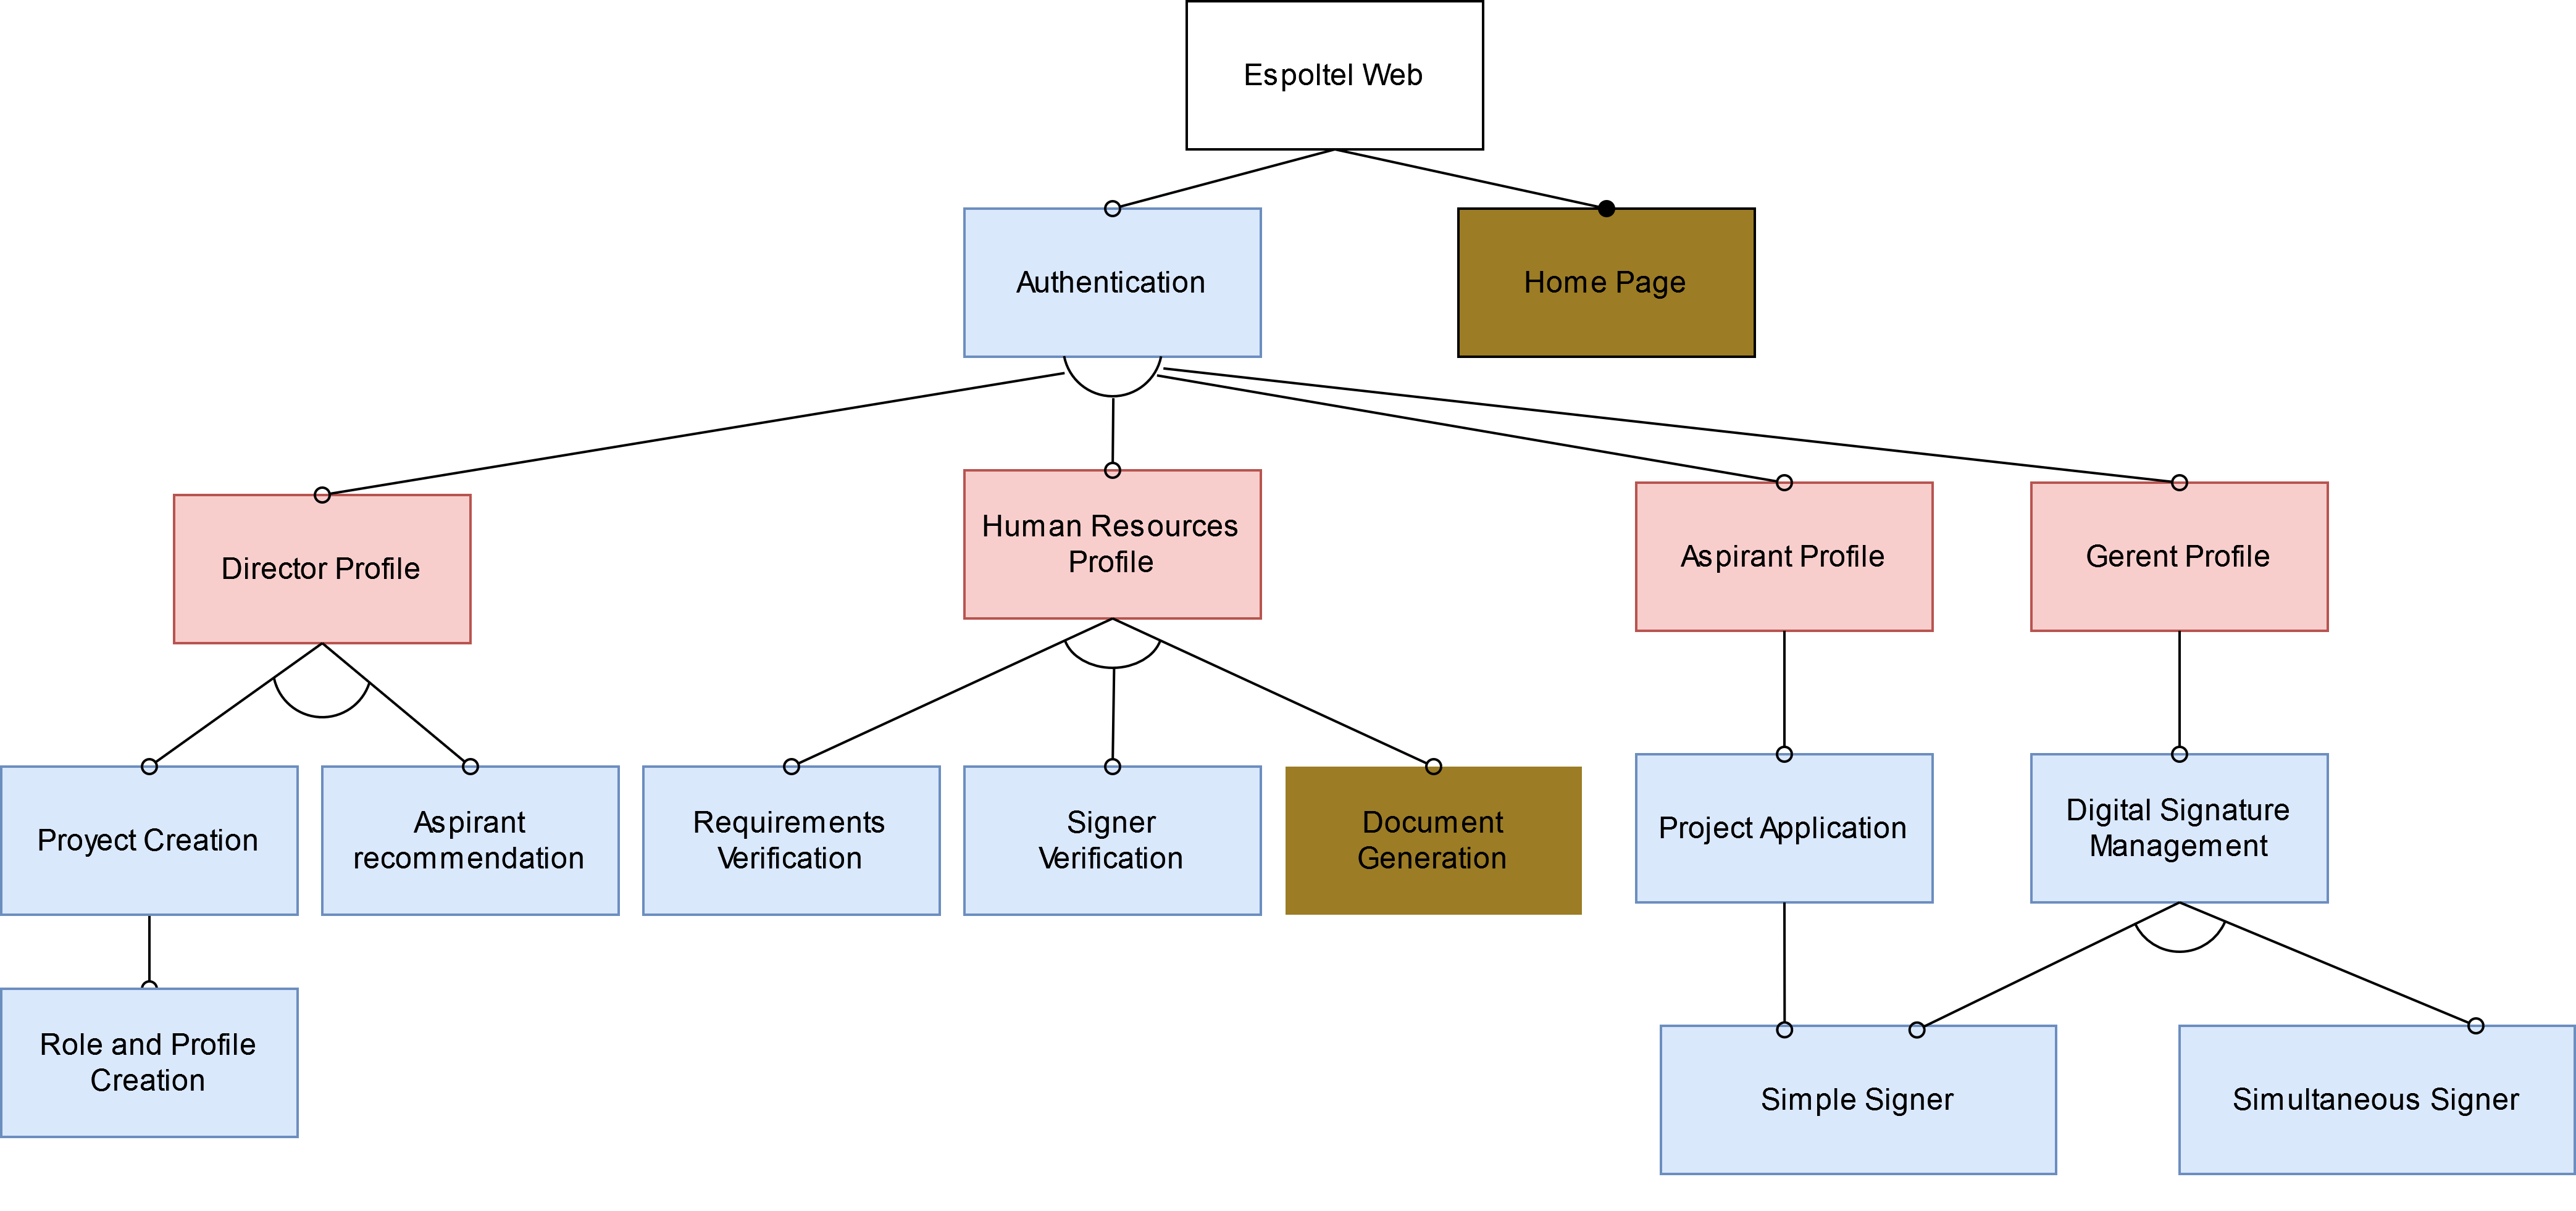
\includegraphics[width=1\textwidth]{ModuleFeaturingWeb.png}
    \caption{Model Featuring Web application}
\end{figure}
\FloatBarrier 
\section{Modules Breakdown}

\setcounter{secnumdepth}{3}
\renewcommand\thesubsubsection{\thesection.\arabic{subsubsection}}
\subsubsection{Home Page Module}
The Home Page module is a component primarily for the users to login in their accounts. It also provides a section to sign up to the system in case of a new user. It's the main entrance to the system.
\subsubsection{Authentication Module}
This module is crucial, as it represents the first layer of system security. Its main function is to verify the authenticity of the user trying to access the system with certain credentials. This module also offers ways to recover a password or a user account through email verifications, in case the user has forgotten any of his credentials. Another important aspect of this module is that it is in charge of identifying which type of user is trying to access the system (directors, managers, aspirants, etc.), authorizing them and redirecting them to the appropriate components.
\subsubsection{Project Creation Module}
The project creation module is a component that belongs to the manager's platform. It allows the manager to create a new project and specify important project data, as well as human talent requirements, explicitly showing the specific profiles and roles to be fulfilled by future aspirants. This project can then be sent to the Human Resources department to be processed and executed by their team.
\subsubsection{Role and Profile Creation Module}
This sub-module of the project creation module allows the project director to quickly and easily define the human talent requirements of the profiles for each role in a given project. These requirements can specify the responsibilities, skills, work experiences of a particular profile for the aspirants. Once defined, the roles and profiles are ready to be sent to human resources for action.
\subsubsection{Aspirant recommendation Module}
This module allows project managers to recommend for a role an aspirant who has previously worked with ESPOLTEL. This recommended aspirant has priority in the hiring process.
\subsubsection{Requirements Verification Module}
This is an important component for the human resources team. It is necessary for verifying the integrity and requirements of a project defined by a director. Human resources is in charge of the whole project structure review and the profiles requested by the director. This department should also manage the incoming aspirants and verify the forms and the requested information about them.
\subsubsection{Signer Verification Module}
Module that goes hand in hand with the digital signature management module, allows the human resources role to verify that the aspirant's signature is valid on documents such as contracts or confidential agreements.
\subsubsection{Document Generation Module}
The generation of documents is a module used by Human Resources that generates formatted documents from determinate templates for all of the processes involved in an application. Basically, after the documents and information verification are completed, it is necessary to create documents such as contracts or approvals that need to be signed by the manager and aspirants. This module is in charge of generating these documents in their correct format and then sending them to the roles involved (managers and aspirants).
\subsubsection{Project Application Module}
This module is essentially made for the aspirants to fill out the forms and data required for submitting their application. The aspirant will be able to visualize all the projects available posted by directors with the corresponding profiles and roles needed. Then the aspirant can start an application for any project by providing corresponding information, such as a resume and identity forms. After the application is completed, it is going to be sent to Human Resources so they to verifythe information and start the process of profile of the roles selection.
\subsubsection{Digital Signature Management Module}
The Digital Signature Management Module allows the manager to select in which way they want to sign documents (one by one or multiple signing). 
\subsubsection{Simple Signer Module}
Allows the manager and aspirants to electronically sign a single document. It's necessary to input the credentials before sign a document.
\subsubsection{Simultaneous Signer Module}
Allows only the manager to sign multiple documents for once. It's necessary to input the credentials one single time for signing all of the documents.
\section{Module Featuring: Mobile application}



\begin{figure}
    \centering \small
    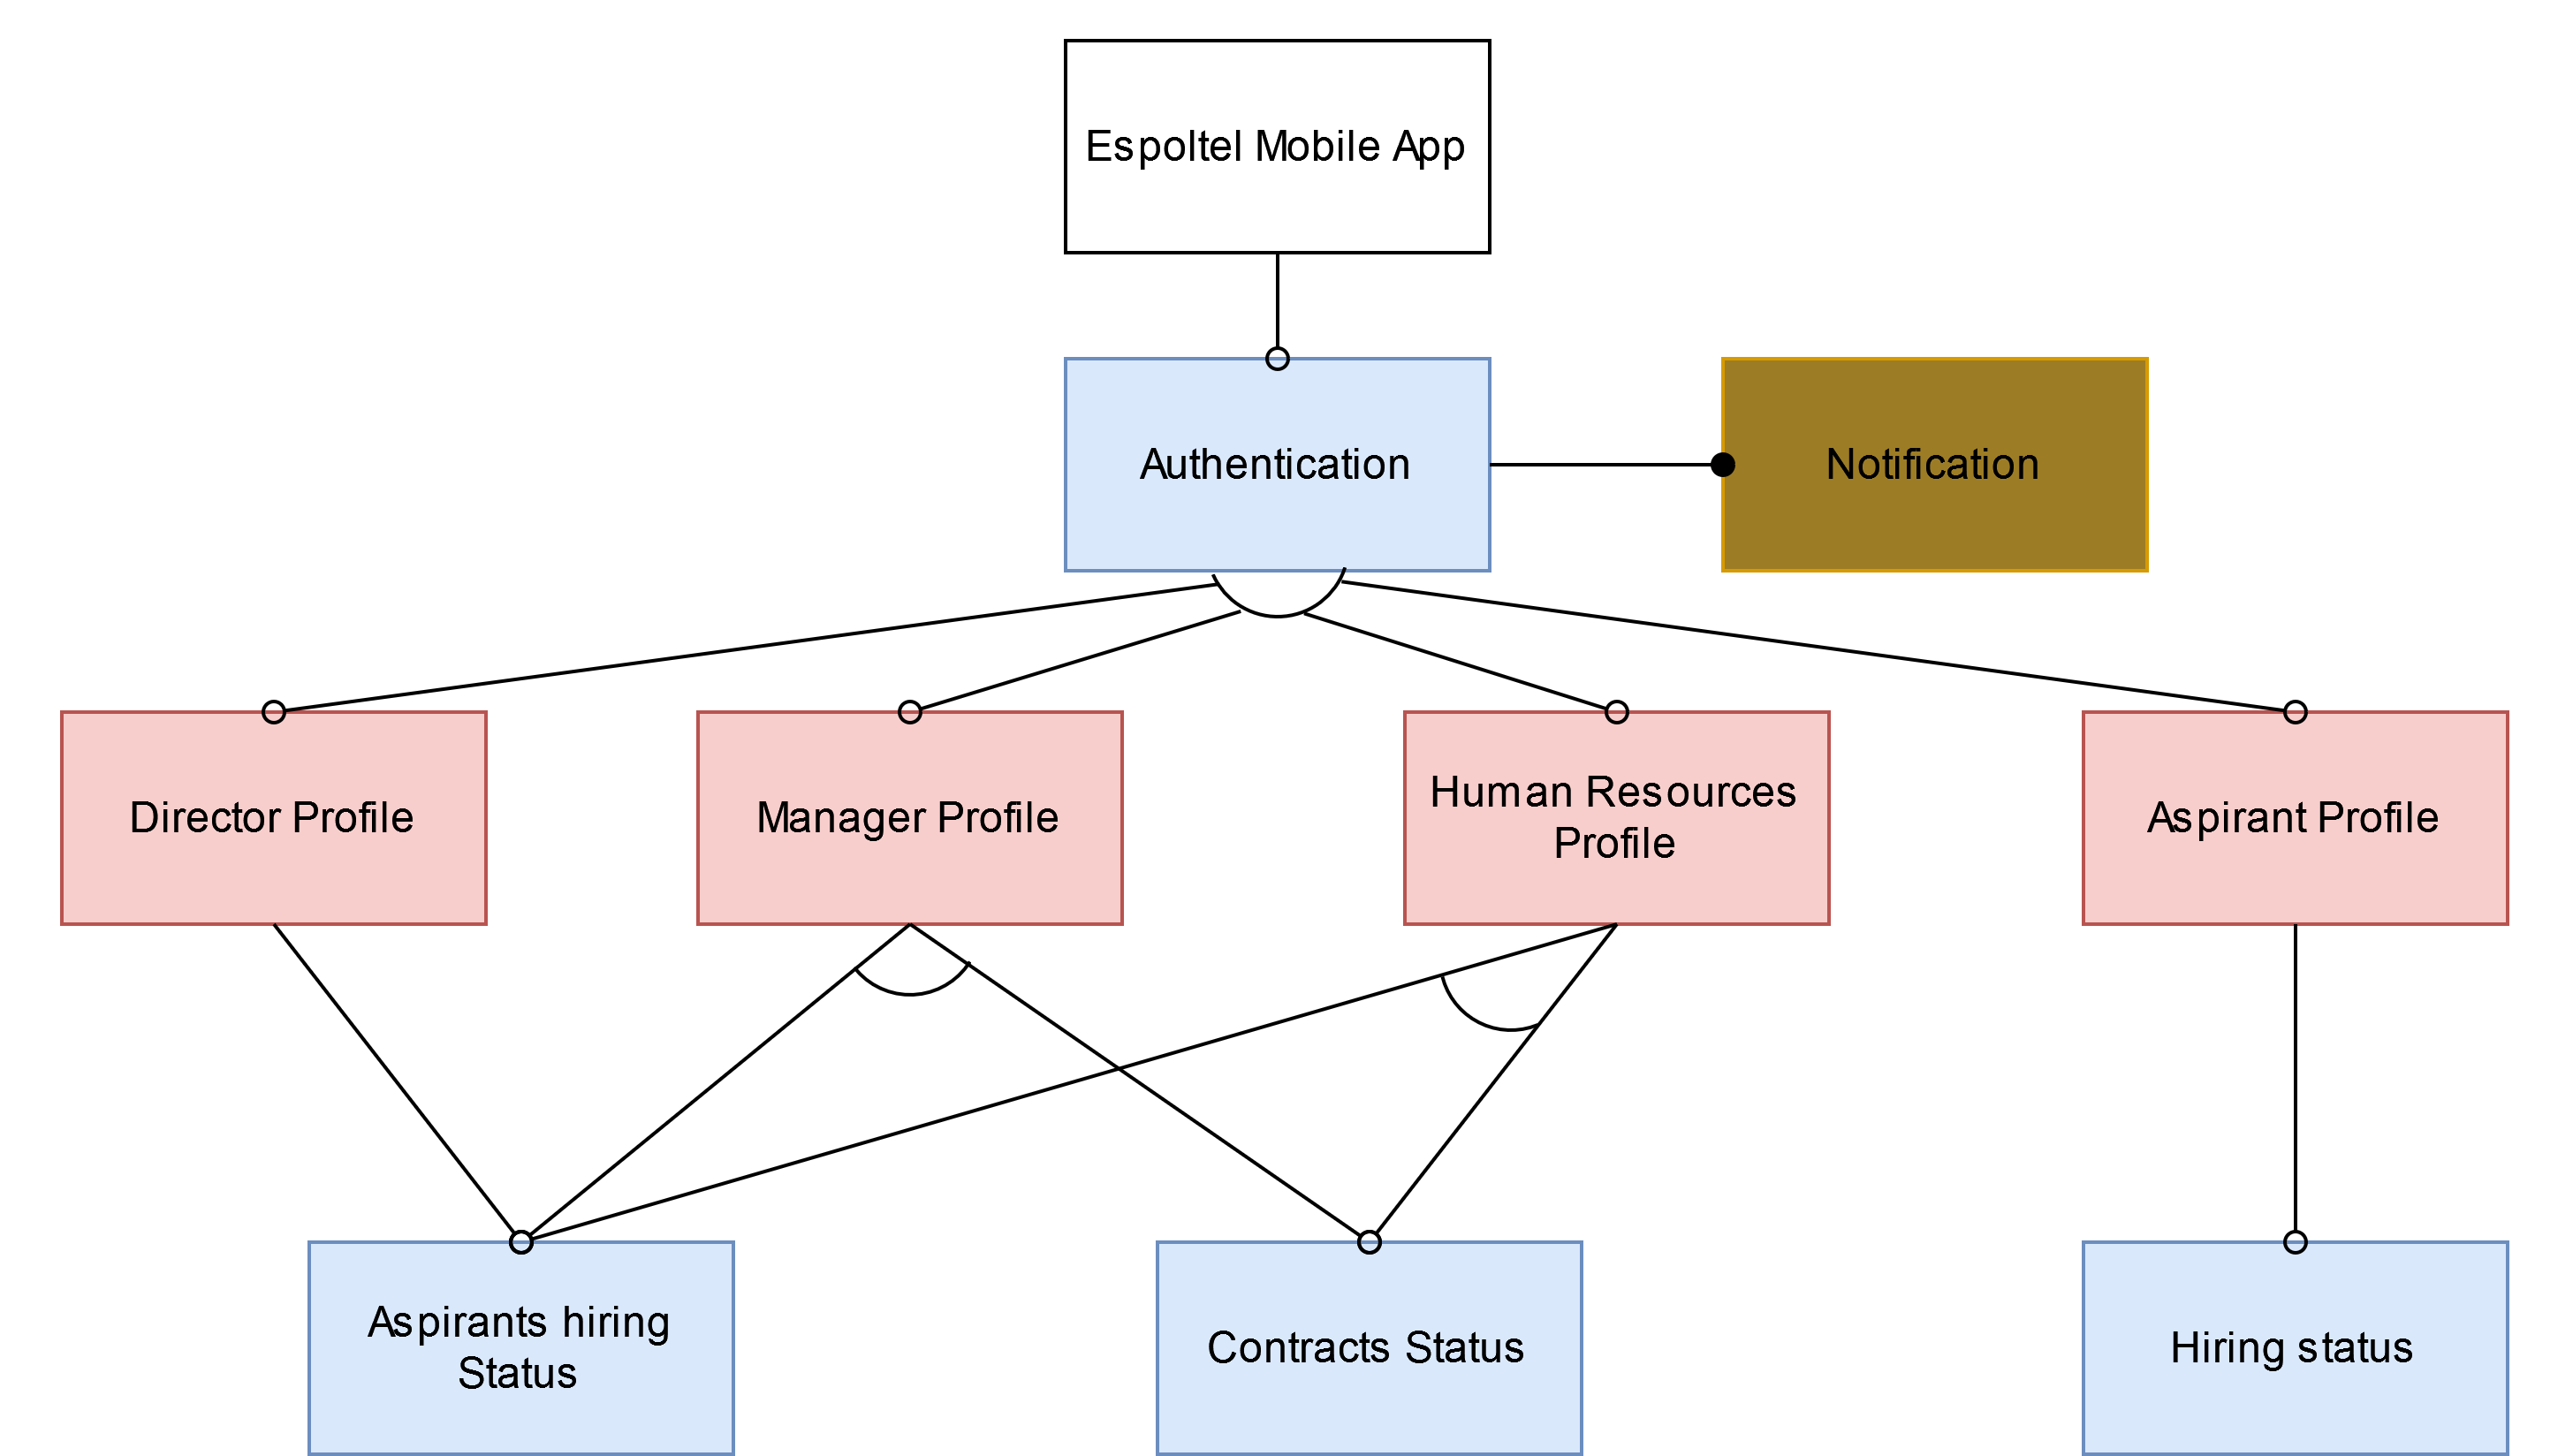
\includegraphics[width=\textwidth]{ModuleFeaturingMobile.png}
    \caption{Model Featuring Web application}
    \label{fig:module_featuring_mobile}
\end{figure}



\FloatBarrier 

\section{Modules Breakdown}
\setcounter{secnumdepth}{3}
\renewcommand\thesubsubsection{\thesection.\arabic{subsubsection}}


\subsubsection {Home Page Module}
The Home Page module let the users to input their credentials for getting into the system. For the mobile application is mandatory to already have an account created since there's no option for signing up.
\subsubsection{Authentication Module}
This module is crucial as it represents the first layer of security of the system. It's main duty is to verify the authenticity of the user trying to log in to the system with some particular credentials. This module also offers ways of recovering a password or a user account through email verifications, in case the user has forgotten any of their credentials. Another important aspect about this module, is that is the one in charge of identifying what type of user is trying to enter to the system (directors, managers, aspirants, etc.) and redirect them to the correct controls.
\subsubsection{Notification Module}
This module is crucial for the mobile app, as it's the main reason for developing the app. This component has to notify the manager if they have any pending signing of documents and show how many. Also, this module tracks the evolution of a project and notifies the manager if any process is incomplete and it's approaching the deadline. At the same time, the notification module serves the aspirants and directors as a notifier on any updates towards the aspirants and selection process.
\subsubsection{Contract Status Module}
This component tracks the status of the contracts generated by human resources for the aspirants. If any change is detected, it notifies the director, aspirant, and manager about what was updated.
\subsubsection{Hiring Status Module}
This component tracks the status of one aspirant, whether aspirant has followed the hiring flow, and the current status is in. It would also tell the applicant what he/she has to do to go to the next phase.
\subsubsection{Aspirants Hiring Status Module}
This component tracks the status of all applicants, their status in the hiring flow and their current status. It also indicates in which project they are applying for the projects that the directors or managers are in charge of.

\chapter{User stories (Functional requirements)}
\section{Web application}
\subsection{Must}
%%
\begin{table}[H]

\centering \small
\resizebox{\textwidth}{!}{   \begin{tabularx}{\textwidth}{|l|X|}
\hline
\textbf{Identifier} & WM1 \\ \hline
\textbf{Priority} & 1 \\ \hline
\textbf{Dependencies} & None \\ \hline
\textbf{Version} & V1.0 \\ \hline
\textbf{Description} & As an aspirant, I must be able to digitally sign my contract and confidentiality agreement so that I can complete the paperwork required for my hiring.\\ \hline
\textbf{Reverse Card} & 
\begin{itemize}
   \item The product needs to use FirmaEC's external module to ensure security in digital signatures.
    \item The aspirant must have a token loaded in the product.
    \item Signers must enter their credentials associated with their token before they can sign.
\end{itemize} \\ \hline
\end{tabularx} }
\caption{User Story: Simple Signer (Web application)}
\label{tab:wm1}
\end{table} \FloatBarrier 
%%

%%
\begin{table}[H]

\centering \small
\resizebox{\textwidth}{!}{   \begin{tabularx}{\textwidth}{|l|X|}
\hline
\textbf{Identifier} & WM2 \\ \hline
\textbf{Priority} & 1 \\ \hline
\textbf{Dependencies} & None \\ \hline
\textbf{Version} & V1.0 \\ \hline
\textbf{Description} & As an aspirant, I must be able to apply for a role in a project of interest in which I qualify for the requested profile. In order to be able to get my role of interest.\\ \hline
\textbf{Reverse Card} & 
\begin{itemize}
    \item Most projects are not public, so only authorized personnel can see them.
    \item The aspirant must be notified if his or her application has been accepted.
    \item The product must support concurrency of multiple aspirants and synchronize them in the order of events.
\end{itemize} \\ \hline
\end{tabularx} }
\caption{User Story: Aspirant application (Web application)}
\label{tab:wm2}
\end{table} \FloatBarrier 
% end User history 2

% User history 3
\begin{table}[H]

\centering \small
\resizebox{\textwidth}{!}{   \begin{tabularx}{\textwidth}{|l|X|}
\hline
\textbf{Identifier} & WM3 \\ \hline
\textbf{Priority} & 1 \\ \hline
\textbf{Dependencies} & None \\ \hline
\textbf{Version} & V1.0 \\ \hline
\textbf{Description} & As a member of Human Resources, I must have to validate the electronic signatures of applicants, to ensure that contracts and agreements are formalized.\\ \hline
\textbf{Reverse Card} & 
\begin{itemize}
     \item The product needs to use FirmaEC's external module to ensure security in digital signs.
     \item Document signature verification should not take more than one minute.
\end{itemize} \\ \hline
\end{tabularx} }
\caption{User Story: Sign validation (Web application)}
\label{tab:wm3}
\end{table} \FloatBarrier 
% end User history 3
% User history 4
\begin{table}[H]
\centering \small

\resizebox{\textwidth}{!}{   \begin{tabularx}{\textwidth}{|l|X|}
\hline
\textbf{Identifier} & WM4 \\ \hline
\textbf{Priority} & 1 \\ \hline
\textbf{Dependencies} & None \\ \hline
\textbf{Version} & V1.0 \\ \hline
\textbf{Description} & As a manager, I must have to be able to digitally sign multiple documents, such as contracts or confidentiality agreements, simultaneously, so that I can save time and work more efficiently.\\ \hline
\textbf{Reverse Card} & 
\begin{itemize}
    \item The product needs to use FirmaEC's external module to ensure security in digital signs.
    \item The manager must have a token loaded in the product.
    \item Signers must put their credentials associated with their token before they can sign.
\end{itemize} \\ \hline
\end{tabularx} }
\caption{User Story: Simultaneous Signer (Web application)}
\label{tab:wm4}
\end{table} \FloatBarrier 
% end User history 4

%%
\begin{table}[H]
\centering \small

\resizebox{\textwidth}{!}{   \begin{tabularx}{\textwidth}{|l|X|}
\hline
\textbf{Identifier} & WM5 \\ \hline
\textbf{Priority} & 1 \\ \hline
\textbf{Dependencies} & None \\ \hline
\textbf{Version} & V1.0 \\ \hline
\textbf{Description} & As an aspirant, I must be able to upload my digital certificate to the platform so that I can sign multiple documents such as contracts or confidentiality agreements for the projects I have applied for. \\ \hline
\textbf{Reverse Card} & 
\begin{itemize}
    \item The product needs to ensure that the digital certificate is uploaded securely and can be validated during the signing process.
    \item The aspirant must be able to use their digital certificate to sign documents without additional manual input.
    \item The product could store in a very secure database this file for future signatures.
    \item It must be validated that it is a correct certificate.
\end{itemize} \\ \hline
\end{tabularx} }
\caption{User Story: Digital Certificate Upload for Aspirants (Web application)}
\label{tab:wm5}
\end{table} \FloatBarrier 
%%
%%
% User history - Manager Digital Certificate Upload (Web application)
\begin{table}[H]
\centering \small

\resizebox{\textwidth}{!}{   \begin{tabularx}{\textwidth}{|l|X|}
\hline
\textbf{Identifier} & WM6 \\ \hline
\textbf{Priority} & 1 \\ \hline
\textbf{Dependencies} & None \\ \hline
\textbf{Version} & V1.0 \\ \hline
\textbf{Description} & As a manager, I must be able to upload my digital certificate to the platform so that I can sign multiple documents such as contracts or confidentiality agreements for the projects I am managing. \\ \hline
\textbf{Reverse Card} & 
\begin{itemize}
    \item The product needs to ensure that the digital certificate is uploaded securely and can be validated during the signing process.
    \item The manager must be able to use their digital certificate to sign documents without additional manual input.
    \item The platform must verify the authenticity of the certificate before allowing document signing
    \item The product could store in a very secure database this file for future signatures.
\end{itemize} \\ \hline
\end{tabularx} }
\caption{User Story: Digital Certificate Upload for Managers (Web application)}
\label{tab:wm6}
\end{table} \FloatBarrier 
% end User history - Manager Digital Certificate Upload (Web application)

%%

\begin{table}[H]
	\centering
	\small
	\resizebox{\textwidth}{!}{ \begin{tabularx}{\textwidth}{|l|X|}
			\hline
			\textbf{Identifier} & WM7 \\ \hline
			\textbf{Priority} & 1 \\ \hline
			\textbf{Dependencies} & None \\ \hline
			\textbf{Version} & V1.0 \\ \hline
			\textbf{Description} & As a Director, Member of Human Resources, or Manager, I must be able to view the hirings or personnel associated with a project, so I can have an overview of the team composition and track the progress of recruitment. \\ \hline
			\textbf{Reverse Card} &
			\begin{itemize}
				\item The system must provide a view that lists all personnel associated with a project, including their roles, profiles and hiring status.
				\item The view should allow filtering and sorting of personnel by different criteria (e.g., role, status, date of hiring).
				\item The system should display relevant information for each person, such as their name, role, their hiring status.
				\item Access to this view should be restricted to authorized users with Director, HR, or Manager roles.
			\end{itemize} \\ \hline
	\end{tabularx} }
	\caption{User Story: View Hirings or Personnel (Web application)}
	\label{tab:wm7}
\end{table} \FloatBarrier

\begin{table}[H]
	\centering
	\small
	\resizebox{\textwidth}{!}{ \begin{tabularx}{\textwidth}{|l|X|}
			\hline
			\textbf{Identifier} & WM8 \\ \hline
			\textbf{Priority} & 2 \\ \hline
			\textbf{Dependencies} & WS3 \\ \hline
			\textbf{Version} & V1.0 \\ \hline
			\textbf{Description} & As a Director or Manager, I want to be able to view the resources and budget allocated to my project, so I can track project expenses and resource utilization. \\ \hline
			\textbf{Reverse Card} &
			\begin{itemize}
				\item The system must provide a view that displays the budget allocated to the project.
				\item Access to this view should be restricted to authorized users with Director or Manager roles.
			\end{itemize} \\ \hline
	\end{tabularx} }
	\caption{User Story: View Project Resources and Budget (Web application)}
	\label{tab:pb49}
\end{table} \FloatBarrier

\subsection{Should}

%%
\begin{table}[H]
	\centering
	\small
	\resizebox{\textwidth}{!}{ \begin{tabularx}{\textwidth}{|l|X|}
			\hline
			\textbf{Identifier} & WS1 \\ \hline
			\textbf{Priority} & 2 \\ \hline
			\textbf{Dependencies} & None \\ \hline
			\textbf{Version} & V1.1 \\ \hline
			\textbf{Description} & As an aspirant, I should be able to upload my personal documents (such as CV, document ID, certificates, etc.) and pertinent information **by completing forms defined by Human Resources,** to complete the application requirements.\\ \hline
			\textbf{Reverse Card} &
			\begin{itemize}
				\item The files and information must have a database so that the aspirant can update them if required for futures project's.
				\item Human Resources must be able to create and manage the forms that applicants will fill out for pre-hiring and hiring processes.
			\end{itemize} \\ \hline
	\end{tabularx} }
	\caption{User Story: Aspirant information for application (Web application)}
	\label{tab:ws1}
\end{table} \FloatBarrier
%%

%%
\begin{table}[H]
\centering \small

\resizebox{\textwidth}{!}{   \begin{tabularx}{\textwidth}{|l|X|}
\hline
\textbf{Identifier} & WS2 \\ \hline
\textbf{Priority} & 2 \\ \hline
\textbf{Dependencies} & None \\ \hline
\textbf{Version} & V1.0 \\ \hline
\textbf{Description} & As an ESPOLTEL Hiring Manager user, I should be able to create my own account to have access to all controls corresponding to my role, so that my information and permissions are separate from those of other users. \\ \hline
\textbf{Reverse Card} & 
\begin{itemize}
    \item The product must verify the e-mail address in the registration process.
    \item Admin roles account creation process should include role-specific permissions to ensure secure and appropriate access levels.
    \item User data and permissions must be stored in a secure database, with separation of permissions to ensure controls are distinct from other user roles.
\end{itemize} \\ \hline
\end{tabularx} }
\caption{User Story: Account Creation for ESPOLTEL Hiring Manager (Web application)}
\label{tab:ws2}
\end{table} \FloatBarrier 
% end User history 6

%%
\begin{table}[H]
\centering \small
\resizebox{\textwidth}{!}{   \begin{tabularx}{\textwidth}{|l|X|}
\hline
\textbf{Identifier} & WS3\\ \hline
\textbf{Priority} & 2 \\ \hline
\textbf{Dependencies} & None \\ \hline
\textbf{Version} & V1.0 \\ \hline
\textbf{Description} & As a project manager, I want to be able to create a project by defining its name, description, start date, end date,  so that the project’s objectives and timeline are clearly established. \\ \hline
\textbf{Reverse Card} & 
\begin{itemize}
    \item The system must allow the project manager to input detailed information such as the project's name, description, start date, end date, and type.
    \item The product should validate the input dates to ensure the end date is after the start date.
    \item The project manager should be able to edit or delete a project if needed.
\end{itemize} \\ \hline
\end{tabularx} }
\caption{User Story: Project Creation with Details (Web application)}
\label{tab:ws3}
\end{table} \FloatBarrier 
%%

%%
\begin{table}[H]
\centering \small
\resizebox{\textwidth}{!}{   \begin{tabularx}{\textwidth}{|l|X|}
\hline
\textbf{Identifier} & WS4 \\ \hline
\textbf{Priority} & 2 \\ \hline
\textbf{Dependencies} & WS3 \\ \hline
\textbf{Version} & V1.0 \\ \hline
\textbf{Description} & As a project manager, I want to be able to define roles and necessary profiles for the project, including the required skills and experience for each role, so that applicants can understand the requirements and apply for suitable positions. \\ \hline
\textbf{Reverse Card} & 
\begin{itemize}
    \item The system must allow the project manager to specify detailed requirements for each role, such as required skills and experience.
    \item The requirements for each role should be listed in a checklist style for clarity.
    \item The project manager should be able to edit or delete roles and requirements as needed.
\end{itemize} \\ \hline
\end{tabularx} }
\caption{User Story: Role and Profile Definition for Project (Web application)}
\label{tab:ws4}
\end{table} \FloatBarrier 
%%

% User history 8
\begin{table}[H]
\centering \small
\resizebox{\textwidth}{!}{   \begin{tabularx}{\textwidth}{|l|X|}
\hline
\textbf{Identifier} & WS5 \\ \hline
\textbf{Priority} & 2 \\ \hline
\textbf{Dependencies} & None \\ \hline
\textbf{Version} & V1.0 \\ \hline
\textbf{Description} & As a manager or project director of ESPOLTEL, I should be able to monitor the projects under my supervision to maintain better control and make informed decisions. \\ \hline
\textbf{Reverse Card} & 
\begin{itemize}
    \item The system must provide a project overview dashboard for managers, for assigned team members and their hiring progress.
    \item Managers should have access to real-time updates of the hiring process of their team members on their projects.
    \item The product must allow managers to filter and search their projects.

\end{itemize} \\ \hline
\end{tabularx} }
\caption{User Story: Project Monitoring for Managers (Web application)}
\label{tab:ws5}
\end{table} \FloatBarrier 
% end User history 8

% User history 9
\begin{table}[H]
\centering \small
\resizebox{\textwidth}{!}{   \begin{tabularx}{\textwidth}{|l|X|}
\hline
\textbf{Identifier} & WS6 \\ \hline
\textbf{Priority} & 2 \\ \hline
\textbf{Dependencies} & None \\ \hline
\textbf{Version} & V1.0 \\ \hline
\textbf{Description} & As an aspirant, I should be able to monitor the projects I have applied for, to stay updated on their progress and better manage my participation. \\ \hline
\textbf{Reverse Card} & 
\begin{itemize}
    \item The system must provide a project overview dashboard for aspirants, displaying the projects they have applied for.
    \item Aspirants should have access to real-time updates on the status of the projects they have applied for.
    \item The product must allow applicants to filter and search the projects they have applied for.
\end{itemize} \\ \hline
\end{tabularx} }
\caption{User Story: Project Monitoring for Aspirants (Web application)}
\label{tab:ws6}
\end{table} \FloatBarrier 
% end User history 9

% User history 10
\begin{table}[H]
\centering \small
\resizebox{\textwidth}{!}{   \begin{tabularx}{\textwidth}{|l|X|}
\hline
\textbf{Identifier} & WS7 \\ \hline
\textbf{Priority} & 2 \\ \hline
\textbf{Dependencies} & None \\ \hline
\textbf{Version} & V1.0 \\ \hline
\textbf{Description} & As a member of Human Resources, I should be able to generate contracts and agreements from templates, to save time in creating customized documents. \\ \hline
\textbf{Reverse Card} & 
\begin{itemize}
    \item The system must provide the ability to generate contracts and agreements based on pre-defined templates.
    \item The information on these documents was obtained from the forms sent to the applicant.
    \item Other important information in these documents, such as the start and end of the contract, must be configurable.
    \item The document generation should not take more than 5 minutes.
\end{itemize} \\ \hline
\end{tabularx} }
\caption{User Story: Automatic Document Generation (Web application)}
\label{tab:ws7}
\end{table} \FloatBarrier 
% end User history 10

% User history 11
\begin{table}[H]
\centering \small
\resizebox{\textwidth}{!}{   \begin{tabularx}{\textwidth}{|l|X|}
\hline
\textbf{Identifier} & WS8 \\ \hline
\textbf{Priority} & 2 \\ \hline
\textbf{Dependencies} & None \\ \hline
\textbf{Version} & V1.0 \\ \hline
\textbf{Description} & As a Human Resources member, I should be able to verify the requirements based on an applicant's information, to ensure that they meet the necessary qualifications for a project. \\ \hline
\textbf{Reverse Card} & 
\begin{itemize}
    \item Human resources members should be able to access a checklist or list of requirements that can be cross-referenced with the aspirant's provided details.
\end{itemize} \\ \hline
\end{tabularx} }
\caption{User Story: Verifying Applicant Requirements (Web application)}
\label{tab:ws8}
\end{table} \FloatBarrier 
% end User history 11

%%
\begin{table}[H]
\centering \small
\resizebox{\textwidth}{!}{   \begin{tabularx}{\textwidth}{|l|X|}
\hline
\textbf{Identifier} & WS9 \\ \hline
\textbf{Priority} & 1 \\ \hline
\textbf{Dependencies} & None \\ \hline
\textbf{Version} & V1.0 \\ \hline
\textbf{Description} & As a Espoltel Hiring Manager user, I should be able to log into the system securely using my credentials, so that I can access project management features and functionalities. \\ \hline
\textbf{Reverse Card} & 
\begin{itemize}
    \item The system must provide a secure login interface with fields for username and password.
    \item Users should receive error messages for incorrect login attempts.
    \item The login process should be secured using encryption.
\end{itemize} \\ \hline
\end{tabularx} }
\caption{User Story: Secure Login (Web application)}
\label{tab:ws9}
\end{table} \FloatBarrier 
%%

%%
\begin{table}[H]
\centering \small
\resizebox{\textwidth}{!}{   \begin{tabularx}{\textwidth}{|l|X|}
\hline
\textbf{Identifier} & WS10 \\ \hline
\textbf{Priority} & 2 \\ \hline
\textbf{Dependencies} & WS9 \\ \hline
\textbf{Version} & V1.0 \\ \hline
\textbf{Description} & As a ESPOLTEL Hiring Manager user, I should be able to select my role (Aspirant, Project Manager, Project Director, or HR Member) before logging in, so that I can be directed to the appropriate login process and access the specific functionalities related to my role. \\ \hline
\textbf{Reverse Card} & 
\begin{itemize}
    \item The system must provide a role selection interface before the login screen.
    \item Based on the selected role, the system should display a their views.
    \item The system should restrict access based on the selected role, only allowing access to functionalities permitted for each role.
\end{itemize} \\ \hline
\end{tabularx} }
\caption{User Story: Role Selection Before Login (Web application)}
\label{tab:ws10}
\end{table} \FloatBarrier 
%%

%%
\begin{table}[H]
\centering
\small
\resizebox{\textwidth}{!}{   \begin{tabularx}{\textwidth}{|l|X|}
\hline
\textbf{Identifier} & WS11 \\ \hline
\textbf{Priority} & 2 \\ \hline
\textbf{Dependencies} & None \\ \hline
\textbf{Version} & V1.2 \\ \hline
\textbf{Description} & As a member of Human Resources, I should be able to upload contract and agreement formats for generating customized documents for aspirants. \\ \hline
\textbf{Reverse Card} & 
\begin{itemize}
    \item The system must allow the upload of templates categorized by role and hiring profile.
    \item Templates must be stored securely, with role-specific access control.
    \item HR staff should be able to select the appropriate template based on the applicant’s role and profile.
    \item The upload process should validate that the template format is correct and functional, probably in docx format.
\end{itemize} \\ \hline
\end{tabularx} }
\caption{User Story: Upload Templates by Role and Hiring Profile (Web application)}
\label{tab:ws11}
\end{table}
%%

%%
%%
\begin{table}[H]
\centering
\small
\resizebox{\textwidth}{!}{   
    \begin{tabularx}{\textwidth}{|l|X|}
    \hline
    \textbf{Identifier} & WS12 \\ \hline
    \textbf{Priority} & 2 \\ \hline
    \textbf{Dependencies} & None \\ \hline
    \textbf{Version} & V1.0 \\ \hline
    \textbf{Description} & As an aspirant, I should be able to cancel my application for a specific role or hiring profile, so that I can withdraw from a recruitment process if my circumstances change. \\ \hline
    \textbf{Reverse Card} & 
    \begin{itemize}
        \item The system must provide an option for applicants to cancel their application from the user dashboard.
        \item The cancellation process should require the applicant to provide a reason for withdrawal, selected from predefined options (e.g., accepted another offer, change in personal circumstances) or as a custom entry.
        \item Upon cancellation, Human resources and project managers should receive a notification indicating that the applicant has withdrawn from the process.
        \item Once canceled, the product should be flagged as "Withdrawn" and removed from further consideration for that specific role or profile.
        \item Aspirants should not be able to reapply for the same role or profile within a set period (e.g., 30 days) after cancellation.
    \end{itemize} \\ \hline
    \end{tabularx} 
}
\caption{User Story: Applicant Cancels Application for Role or Profile (Web application)}
\label{tab:ws12}
\end{table}
%%
\begin{table}[H]
	\centering
	\small
	\resizebox{\textwidth}{!}{ \begin{tabularx}{\textwidth}{|l|X|}
			\hline
			\textbf{Identifier} & WS13 \\ \hline
			\textbf{Priority} & 2 \\ \hline
			\textbf{Dependencies} & None \\ \hline
			\textbf{Version} & V1.0 \\ \hline
			\textbf{Description} & As a member of Human Resources, I should be able to schedule interviews with applicants, specifying the date, time, and interviewer, so that the selection process can be carried out efficiently. \\ \hline
			\textbf{Reverse Card} &
			\begin{itemize}
				\item The system must allow the selection of applicants, available dates, times, and interviewers for scheduling.
				\item The interviewers should receive a notification with the details of the scheduled interview, including a link or information to access the virtual meeting room if applicable.
				\item The system should allow rescheduling or canceling interviews, with automatic notifications to the involved parties.
				\item Applicants must be notified of their interview schedule via email, including the date, time, interviewer, and instructions for the interview.
				\item The system should prevent scheduling conflicts, such as double-booking an interviewer or applicant at the same time.
			\end{itemize} \\ \hline
	\end{tabularx} }
	\caption{User Story: Schedule Interviews (Web application)}
	\label{tab:ws13}
\end{table} \FloatBarrier
% End User story - Schedule Interviews (Web application)

% User story - Interview Results (Web application)
\begin{table}[H]
	\centering
	\small
	\resizebox{\textwidth}{!}{ \begin{tabularx}{\textwidth}{|l|X|}
			\hline
			\textbf{Identifier} & WS14 \\ \hline
			\textbf{Priority} & 2 \\ \hline
			\textbf{Dependencies} & WS13 \\ \hline
			\textbf{Version} & V1.0 \\ \hline
			\textbf{Description} & As an member of Human Talent, I should be able to record the results and observations of the interviews conducted, including scores and comments, so that there is a formal record of the evaluation of each applicant. \\ \hline
			\textbf{Reverse Card} &
			\begin{itemize}
				\item The system must provide a form for each interview, allowing scores to be entered based on predefined criteria.
				\item Interviewers should be able to add specific comments about the applicant's performance during the interview.
				\item The results and comments must be stored securely and associated with the applicant's profile.
				\item The system should allow authorized users (e.g., HR members, project managers) to access and review the interview results.
			\end{itemize} \\ \hline
	\end{tabularx} }
	\caption{User Story: Record Interview Results}
	\label{tab:ws14}
\end{table} \FloatBarrier
%%

\begin{table}[H]
	\centering
	\small
	\resizebox{\textwidth}{!}{ \begin{tabularx}{\textwidth}{|l|X|}
			\hline
			\textbf{Identifier} & WS15 \\ \hline
			\textbf{Priority} & 2 \\ \hline
			\textbf{Dependencies} & None \\ \hline
			\textbf{Version} & V1.0 \\ \hline
			\textbf{Description} & As a member of Human Resources, I should be able to create and manage forms for pre-hiring and hiring processes, defining the required fields and document uploads, so that applicants can provide the necessary information. \\ \hline
			\textbf{Reverse Card} &
			\begin{itemize}
				\item The system must allow the creation of forms with different field types (text, dropdown, and file).
				\item The system must allow the definition of required document uploads (e.g., CV, ID, certificates).
				item The system must allow upload a word file with a format for generate the documents with this form.
				\item Human Resources must be able to edit and delete existing forms.
			\end{itemize} \\ \hline
	\end{tabularx} }
	\caption{User Story: Form Management for Human Resources (Web application)}
	\label{tab:ws15}
\end{table} \FloatBarrier
%%

\begin{table}[H]
	\centering
	\small
	\resizebox{\textwidth}{!}{ \begin{tabularx}{\textwidth}{|l|X|}
			\hline
			\textbf{Identifier} & WS16 \\ \hline
			\textbf{Priority} & 2 \\ \hline
			\textbf{Dependencies} & WS15 \\ \hline
			\textbf{Version} & V1.0 \\ \hline
			\textbf{Description} & As a member of Human Resources, I want to be able to validate the profiles created by project directors, so that I can edit, approve the profiles and position defined for a project, ensuring they align with company standards and requirements. \\ \hline
			\textbf{Reverse Card} &
			\begin{itemize}
				\item The system must provide a view for Human Resources to review profiles created by project directors.
				\item Human Resources should be able to edit the profile details, such as required skills, and responsibilities, referencial salary.
				\item Human Resources should be able to approve the profiles, making them available for applications.
				\item The system should notify the project director about the status of their profile submission (approved, or pending review).
			\end{itemize} \\ \hline
	\end{tabularx} }
	\caption{User Story: Validate Project Profiles (Web application)}
	\label{tab:pb50}
\end{table} \FloatBarrier

\begin{table}[H]
	\centering
	\small
	\resizebox{\textwidth}{!}{ \begin{tabularx}{\textwidth}{|l|X|}
			\hline
			\textbf{Identifier} & WS17 \\ \hline
			\textbf{Priority} & 2 \\ \hline
			\textbf{Dependencies} &  \\ \hline
			\textbf{Version} & V1.0 \\ \hline
			\textbf{Description} & As an ESPOLTEL Hiring Manager user, I want to be able to search and filter information across the platform, including projects, postulations, format documents, and other relevant data, so that I can quickly find and focus on the data I need. \\ \hline
			\textbf{Reverse Card} &
			\begin{itemize}
				\item The system should allow the combination of multiple filters and the use of search operators within filters.
				\item Users should be able to save frequently used filter and search combinations for quick access.
				\item Filter options should be dynamically updated based on the available data.
				\item Search results should be presented in a clear and organized manner, with relevant context for each result.
				\item The search and filter functionality should be easily accessible from all parts of the application.
				\item The filters must include options for projects, profiles, positions, and contractual relationships.
			\end{itemize} \\ \hline
	\end{tabularx} }
	\caption{User Story: Search and Filter Functionality (Web application)}
	\label{tab:pb51}
\end{table} \FloatBarrier

\subsection{Could}
%%
\begin{table}[H]
\centering \small
\resizebox{\textwidth}{!}{   \begin{tabularx}{\textwidth}{|l|X|}
\hline
\textbf{Identifier} & WC1\\ \hline
\textbf{Priority} & 3 \\ \hline
\textbf{Dependencies} & None \\ \hline
\textbf{Version} & V1.0 \\ \hline
\textbf{Description} & As an aspirant, I should be able to view the contracts for the projects I have applied for and are currently active, so that I can have a clear view of the agreements I have signed. \\ \hline
\textbf{Reverse Card} & 
\begin{itemize}
    \item Applicants should be able to filter and search for specific contracts based on the project or date.
    \item Contracts should be displayed in a readable format on the web application.
\end{itemize} \\ \hline
\end{tabularx} }
\caption{User Story: Viewing Signed Contracts (Web application)}
\label{tab:wc1}
\end{table} \FloatBarrier 
%%

%%
\begin{table}[H]
\centering \small
\resizebox{\textwidth}{!}{   \begin{tabularx}{\textwidth}{|l|X|}
\hline
\textbf{Identifier} & WC2 \\ \hline
\textbf{Priority} & 3 \\ \hline
\textbf{Dependencies} & None \\ \hline
\textbf{Version} & V1.0 \\ \hline
\textbf{Description} & As a Project manager, I could be able to recommend an aspirant who has previously worked for ESPOLTEL for a role in a project, based on their past performance and experience, to have a worker in whom I have confidence in my project.\\ \hline
\textbf{Reverse Card} & 
\begin{itemize}
    \item Recommended aspirants will be given priority in the hiring process.
    \item The product must provide an easy way for Project Managers to send recommendations directly from the system.
\end{itemize} \\ \hline
\end{tabularx} }
\caption{User Story: Recommending an Aspirant for a Project Role (Web application)}
\label{tab:wc2}
\end{table} \FloatBarrier 
%%

%%
\begin{table}[H]
\centering \small
\resizebox{\textwidth}{!}{   \begin{tabularx}{\textwidth}{|l|X|}
\hline
\textbf{Identifier} & WC3 \\ \hline
\textbf{Priority} & 3 \\ \hline
\textbf{Dependencies} & None \\ \hline
\textbf{Version} & V1.0 \\ \hline
\textbf{Description} & As an ESPOLTEL hiring manager user, I could be able to recover my password through a secure and efficient process if I forget it, so that I can regain access to the system and continue with my responsibilities without delay. \\ \hline
\textbf{Reverse Card} & 
\begin{itemize}
    \item The password recovery process should be secure, utilizing verification methods (e.g., email or phone number confirmation).
    \item The product must provide an easy-to-use recovery interface accessible from the login page.
    \item If I do not have access to any of the recovery methods I will be notified that I cannot recover my password.
\end{itemize} \\ \hline
\end{tabularx} }
\caption{User Story: Password Recovery (Web application)}
\label{tab:wc3}
\end{table} \FloatBarrier 
 

%%

%%
\begin{table}[H]
\centering \small
\resizebox{\textwidth}{!}{   \begin{tabularx}{\textwidth}{|l|X|}
\hline
\textbf{Identifier} & WC4 \\ \hline
\textbf{Priority} & 1 \\ \hline
\textbf{Dependencies} & WS2 \\ \hline
\textbf{Version} & V1.0 \\ \hline
\textbf{Description} & As an ESPOLTEL Hiring Manager user, I could be able to verify my email address upon registration, so that I ensure secure access to the system and confirm my identity. \\ \hline
\textbf{Reverse Card} & 
\begin{itemize}
    \item The system should send a verification link or code to the user's email address upon registration.
    \item Users must complete the email verification process before accessing sensitive features.
    \item If the verification code is incorrect the product must inform them.
\end{itemize} \\ \hline
\end{tabularx} }
\caption{User Story: Email Verification (Web application)}
\label{tab:wc4}
\end{table} \FloatBarrier 


%%

%%
\begin{table}[H]
\centering \small
\resizebox{\textwidth}{!}{   \begin{tabularx}{\textwidth}{|l|X|}
\hline
\textbf{Identifier} & WC5\\ \hline
\textbf{Priority} & 3 \\ \hline
\textbf{Dependencies} & None \\ \hline
\textbf{Version} & V1.0 \\ \hline
\textbf{Description} & As an aspirant, I should be able to download the contracts for the projects I have applied for and are currently active, so that I can have a record of the agreements I have signed. \\ \hline
\textbf{Reverse Card} & 
\begin{itemize}
    \item Applicants should be able to download contracts to their devices in a suitable format (e.g., PDF).
\end{itemize} \\ \hline
\end{tabularx} }
\caption{User Story: Downloading Signed Contracts (Web application)}
\label{tab:wc5}
\end{table} \FloatBarrier 
%%

%%
\begin{table}[H]
\centering \small
\resizebox{\textwidth}{!}{   \begin{tabularx}{\textwidth}{|l|X|}
\hline
\textbf{Identifier} & WC6\\ \hline
\textbf{Priority} & 3 \\ \hline
\textbf{Dependencies} & None \\ \hline
\textbf{Version} & V1.0 \\ \hline
\textbf{Description} & As a Human Resources member, I could be able to add private comments on applicant profiles to keep a record of observations and notes during the selection process. \\ \hline
\textbf{Reverse Card} & 
\begin{itemize}
    \item The system should provide a comment section within each applicant's profile accessible only to authorized Human Resources members.
    \item Comments must be saved securely and associated with specific applicants for future reference.
    \item Human Resources should have the ability to edit or delete their own comments as needed.
\end{itemize} \\ \hline
\end{tabularx} }
\caption{User Story: Add Private Comments on Applicant Profiles (Web application)}
\label{tab:wc6}
\end{table} \FloatBarrier 
%%


\begin{table}[H]
	\centering
	\small
	\resizebox{\textwidth}{!}{ \begin{tabularx}{\textwidth}{|l|X|}
			\hline
			\textbf{Identifier} & WC7 \\ \hline
			\textbf{Priority} & 2 \\ \hline
			\textbf{Dependencies} & WS14,  WS8\\ \hline
			\textbf{Version} & V1.0 \\ \hline
			\textbf{Description} & As a member of Human Resources, I want to be able to select the best aspirants based on interview results and fulfillment of requirements, so that I can identify the most suitable candidates for each profile. \\ \hline
			\textbf{Reverse Card} &
			\begin{itemize}
				\item The system must allow filtering of applicants based on the fulfillment of defined requirements (e.g., skills, experience, documents).
				\item The system must allow the selection of multiple applicants for a single role.
			\end{itemize} \\ \hline
	\end{tabularx} }
	\caption{User Story: Selection of Best Applicants (Web application)}
	\label{tab:wc7}
\end{table} \FloatBarrier


\subsection{Won't}

%%
\begin{table}[H]
\centering \small
\resizebox{\textwidth}{!}{   \begin{tabularx}{\textwidth}{|l|X|}
\hline
\textbf{Identifier} & WW1 \\ \hline
\textbf{Priority} & 4 \\ \hline
\textbf{Dependencies} & None \\ \hline
\textbf{Version} & V1.0 \\ \hline
\textbf{Description} & As an ESPOLTEL Hiring Manager administrator, I won't be allow to aspirants view projects they have not applied for, in order to protect the company’s private information. \\ \hline
\textbf{Reverse Card} & 
\begin{itemize}
    \item The system must restrict aspirants access to only those projects for which they have submitted an application.
    \item The product should notify applicants when attempting to access restricted projects, maintaining confidentiality of project information.
    \item Nor would it be possible to see projects that have already passed the contracting period.
\end{itemize} \\ \hline
\end{tabularx} }
\caption{User Story: Restricting Access to Unapplied Projects (Web application)}
\label{tab:ww1}
\end{table} \FloatBarrier 
%%

%%
\begin{table}[H]
\centering \small
\resizebox{\textwidth}{!}{   \begin{tabularx}{\textwidth}{|l|X|}
\hline
\textbf{Identifier} & WW2 \\ \hline
\textbf{Priority} & 4 \\ \hline
\textbf{Dependencies} & None \\ \hline
\textbf{Version} & V1.0 \\ \hline
\textbf{Description} & As an applicant, I won’t be able to edit my application once it has been submitted, to ensure the integrity of the information provided to managers and human resources.\\ \hline
\textbf{Reverse Card} & 
\begin{itemize}
   \item The system must block the editing of applications once they have been submitted.
    \item Applicants should receive a notification indicating that no changes can be made after submission.
    \item Human Resources should be able to view the original version of the application without any subsequent modifications.
\end{itemize} \\ \hline
\end{tabularx} }
\caption{User Story: Prevent Editing of Submitted Application (Web application)}
\label{tab:ww2}
\end{table} \FloatBarrier 
%%

%%
\begin{table}[H]
\centering \small
\resizebox{\textwidth}{!}{   \begin{tabularx}{\textwidth}{|l|X|}
\hline
\textbf{Identifier} & WW3 \\ \hline
\textbf{Priority} & 4 \\ \hline
\textbf{Dependencies} & None \\ \hline
\textbf{Version} & V1.0 \\ \hline
\textbf{Description} & As an applicant, I won’t be able to view projects that are in draft status or have not been officially approved by management, to protect the confidentiality of projects that are not yet available to the public. \\ \hline
\textbf{Reverse Card} & 
\begin{itemize}
   \item The system must restrict the visibility of projects in draft or unapproved status to only authorized internal users.
    \item Applicants attempting to access restricted projects should see a notification indicating that the project is not available for viewing.
    \item The product should only display projects with approved and public status to applicants.
\end{itemize} \\ \hline
\end{tabularx} }
\caption{User Story: Restrict Viewing of Draft or Unapproved Projects (Web application)}
\label{tab:ww3}
\end{table} \FloatBarrier 
%%
%%
\begin{table}[H]
\centering \small
\resizebox{\textwidth}{!}{   \begin{tabularx}{\textwidth}{|l|X|}
\hline
\textbf{Identifier} & WW4 \\ \hline
\textbf{Priority} & 4 \\ \hline
\textbf{Dependencies} & None \\ \hline
\textbf{Version} & V1.0 \\ \hline
\textbf{Description} & As a member of Human Resources, I won’t be able to upload additional documents for each applicant once the application has been approved, to ensure that the hiring process follows a controlled flow without post-approval modifications. \\ \hline
\textbf{Reverse Card} & 
\begin{itemize}
   \item The system must lock document uploads for an applicant once their application status changes to "approved."
    \item Human Resources members attempting to upload documents after approval should see a notification explaining that additional uploads are restricted.
    \item The product should allow only pre-approved or initial documents to be accessible post-approval for compliance.
\end{itemize} \\ \hline
\end{tabularx} }
\caption{User Story: Restrict Additional Document Uploads Post-Approval (Web application)}
\label{tab:ww4}
\end{table} \FloatBarrier 
%%

\section{Mobile application}
\subsection{Must}
% User history 15
\begin{table}[H]
\centering \small
\resizebox{\textwidth}{!}{   \begin{tabularx}{\textwidth}{|l|X|}
\hline
\textbf{Identifier} & MM1 \\ \hline
\textbf{Priority} & 1 \\ \hline
\textbf{Dependencies} & None \\ \hline
\textbf{Version} & V1.0 \\ \hline
\textbf{Description} & As a user of the ESPOLTEL Hiring Manager mobile application, I need to receive notifications for any important events in the hiring process, so that I can stay informed and respond promptly. \\ \hline
\textbf{Reverse Card} & 
\begin{itemize}
    \item The system must send real-time notifications for key events in the hiring process, such as new applicant submissions, documents pending signature, etc. Depending on the role
    \item Users should have the option to customize the types of notifications they receive based on their preferences.
    \item Notifications can be configured to occur at one time of the day or at various periods of the day
    \item The product must ensure that notifications are clear, concise, and provide direct links to relevant information within the mobile application.
\end{itemize} \\ \hline
\end{tabularx} }
\caption{User Story: Mobile Notifications (Mobile application)}
\label{tab:mm1}
\end{table} \FloatBarrier 
% end User history 15

\subsection{Should}
% User history 16
\begin{table}[H]
\centering \small
\resizebox{\textwidth}{!}{   \begin{tabularx}{\textwidth}{|l|X|}
\hline
\textbf{Identifier} & MS1 \\ \hline
\textbf{Priority} & 2 \\ \hline
\textbf{Dependencies} & None \\ \hline
\textbf{Version} & V1.0 \\ \hline
\textbf{Description} & As an aspirant, I should be able to monitor on my smartphone the projects I have applied for, to stay updated on their progress and better manage my participation. \\ \hline
\textbf{Reverse Card} & 
\begin{itemize}
    \item The system must provide a project overview dashboard for aspirants, displaying the projects they have applied for.
    \item Applicants should have access to real-time updates on the status of the projects they have applied for.
    \item The product must allow applicants to filter and search the projects they have applied for.
\end{itemize} \\ \hline
\end{tabularx} }
\caption{User Story: Project Monitoring for Aspirants (Mobile application)}
\label{tab:ms1}
\end{table} \FloatBarrier 
% end User history 16

% User history 17
\begin{table}[H]
\centering \small
\resizebox{\textwidth}{!}{   \begin{tabularx}{\textwidth}{|l|X|}
\hline
\textbf{Identifier} & MS2 \\ \hline
\textbf{Priority} & 2 \\ \hline
\textbf{Dependencies} & None \\ \hline
\textbf{Version} & V1.0 \\ \hline
\textbf{Description} & As a manager or project director of ESPOLTEL, I should be able to monitor on my smartphone the projects under my supervision to maintain better control and make informed decisions. \\ \hline
\textbf{Reverse Card} & 
\begin{itemize}
    \item The system must provide a project overview dashboard for managers, for assigned team members and their hiring progress.
    \item Managers should have access to real-time updates of the hiring process of their team members on their projects.
    \item The product must allow managers to filter and search their project.
\end{itemize} \\ \hline
\end{tabularx} }
\caption{User Story: Project Monitoring for Managers (Mobile application)}
\label{tab:ms2}
\end{table} \FloatBarrier 
%%

%%
\begin{table}[H]
\centering \small
\resizebox{\textwidth}{!}{   \begin{tabularx}{\textwidth}{|l|X|}
\hline
\textbf{Identifier} & MS3 \\ \hline
\textbf{Priority} & 2 \\ \hline
\textbf{Dependencies} & None \\ \hline
\textbf{Version} & V1.0 \\ \hline
\textbf{Description} & As an applicant or manager, I should have access to confidential contracts or agreements that are pending my signature, so that I can review and digitally sign them within the web application. \\ \hline
\textbf{Reverse Card} & 
\begin{itemize}
    \item Users should be able to review the full content of each contract or agreement before signing.
\end{itemize} \\ \hline
\end{tabularx} }
\caption{User Story: Accessing Pending Documents (Mobile application)}
\label{tab:ms3}
\end{table} \FloatBarrier 
% end User history 18

%%
\begin{table}[H]
\centering \small
\resizebox{\textwidth}{!}{   \begin{tabularx}{\textwidth}{|l|X|}
\hline
\textbf{Identifier} & MS4 \\ \hline
\textbf{Priority} & 2 \\ \hline
\textbf{Dependencies} & None \\ \hline
\textbf{Version} & V1.0 \\ \hline
\textbf{Description} & As an ESPOLTEL Hiring Manager user, I should be able to create my own account using the mobile application, so that I can access all controls corresponding to my role, and ensure that my information and permissions are separated from those of other users. \\ \hline
\textbf{Reverse Card} & 
\begin{itemize}
    \item The mobile application must verify the e-mail address during the registration process.
    \item Admin roles account creation process should include role-specific permissions to ensure secure and appropriate access levels.
    \item User data and permissions must be stored securely in the database, with separation of permissions to ensure controls are distinct from other user roles.
\end{itemize} \\ \hline
\end{tabularx} }
\caption{User Story: Account Creation for ESPOLTEL Hiring Manager (Mobile Application)}
\label{tab:ms4}
\end{table} \FloatBarrier 
%%


%%
\begin{table}[H]
\centering \small
\resizebox{\textwidth}{!}{   \begin{tabularx}{\textwidth}{|l|X|}
\hline
\textbf{Identifier} & MS5 \\ \hline
\textbf{Priority} & 2 \\ \hline
\textbf{Dependencies} & None \\ \hline
\textbf{Version} & V1.0 \\ \hline
\textbf{Description} & As an ESPOLTEL user, I should be able to log into the system securely using my credentials on my mobile device, so that I can access the appropriate features and functionalities based on my user role. \\ \hline
\textbf{Reverse Card} & 
\begin{itemize}
    \item The mobile application must provide a secure login interface with fields for username and password.
    \item Users should receive error messages for incorrect login attempts.
    \item The login process should be secured using encryption to protect user data.
\end{itemize} \\ \hline
\end{tabularx} }
\caption{User Story: Secure Login (Mobile Application)}
\label{tab:ms5}
\end{table} \FloatBarrier 
%%

%%
\begin{table}[H]
\centering \small
\resizebox{\textwidth}{!}{   \begin{tabularx}{\textwidth}{|l|X|}
\hline
\textbf{Identifier} & MS6 \\ \hline
\textbf{Priority} & 2 \\ \hline
\textbf{Dependencies} & MS5 \\ \hline
\textbf{Version} & V1.0 \\ \hline
\textbf{Description} & As an ESPOLTEL user, I should be able to select my role (Aspirant, Project Manager, Project Director, or HR Member) on my mobile device before logging in, so that I can be directed to the specific features and functionalities relevant to my role. \\ \hline
\textbf{Reverse Card} & 
\begin{itemize}
    \item The mobile application must provide a role selection interface before the login screen.
    \item Based on the selected role, the mobile application should display a role-specific view after login.
    \item Access to functionalities should be restricted based on the selected role, allowing only those permitted for each role.
\end{itemize} \\ \hline
\end{tabularx} }
\caption{User Story: Role Selection Before Login (Mobile Application)}
\label{tab:ms6}
\end{table} \FloatBarrier 
%%

\begin{table}[H]
\centering \small
\resizebox{\textwidth}{!}{   \begin{tabularx}{\textwidth}{|l|X|}
\hline
\textbf{Identifier} & WS8 \\ \hline
\textbf{Priority} & 2 \\ \hline
\textbf{Dependencies} & None \\ \hline
\textbf{Version} & V1.0 \\ \hline
\textbf{Description} & As a Human Resources member, I should be able to view applicants by specific skills and experience to facilitate the selection of candidates who meet the project requirements. \\ \hline
\textbf{Reverse Card} & 
\begin{itemize}
   \item The system must provide a filtering feature in the applicant list that allows Human Resources to search by skills and experience.
    \item Human Resources should be able to apply multiple filters simultaneously to refine the candidate list.
    \item The system should display only applicants that match the selected criteria for easy review.
\end{itemize} \\ \hline
\end{tabularx} }
\caption{User Story: Filter Applicants by Skills and Experience (Web application)}
\label{tab:WS8}
\end{table} \FloatBarrier 
%%


\subsection{Could}

%%
\begin{table}[H]
\centering \small
\resizebox{\textwidth}{!}{   \begin{tabularx}{\textwidth}{|l|X|}
\hline
\textbf{Identifier} & MC1\\ \hline
\textbf{Priority} & 3 \\ \hline
\textbf{Dependencies} & None \\ \hline
\textbf{Version} & V1.0 \\ \hline
\textbf{Description} & As an aspirant, I could be able to view the contracts for the projects I have applied for and are currently active on my smartphone, so that I can have a clear view of the agreements I have signed. \\ \hline
\textbf{Reverse Card} & 
\begin{itemize}
    \item Applicants should be able to filter and search for specific contracts based on the project or date.
    \item Contracts should be displayed in a readable format on the smartphone screen.
\end{itemize} \\ \hline
\end{tabularx} }
\caption{User Story: Viewing Signed Contracts (Mobile application)}
\label{tab:mc1a}
\end{table} \FloatBarrier 
%%

%%
\begin{table}[H]
\centering \small
\resizebox{\textwidth}{!}{   \begin{tabularx}{\textwidth}{|l|X|}
\hline
\textbf{Identifier} & MC2 \\ \hline
\textbf{Priority} & 3 \\ \hline
\textbf{Dependencies} & None \\ \hline
\textbf{Version} & V1.0 \\ \hline
\textbf{Description} & As an ESPOLTEL hiring manager user, I could be able to recover my password through a secure and efficient process via email from my mobile device if I forget it, so that I can regain access to the system and continue with my responsibilities without delay. \\ \hline
\textbf{Reverse Card} & 
\begin{itemize}
    \item The password recovery process should be secure, utilizing email verification methods.
    \item The product must provide an easy-to-use recovery interface accessible from the mobile login page.
    \item If I do not have access to my email, I will be notified that I cannot recover my password.
\end{itemize} \\ \hline
\end{tabularx} }
\caption{User Story: Password Recovery (Mobile application)}
\label{tab:mc2}
\end{table} \FloatBarrier 
%%

%%
\begin{table}[H]
\centering \small
\resizebox{\textwidth}{!}{   \begin{tabularx}{\textwidth}{|l|X|}
\hline
\textbf{Identifier} & MC3 \\ \hline
\textbf{Priority} & 1 \\ \hline
\textbf{Dependencies} & WS2 \\ \hline
\textbf{Version} & V1.0 \\ \hline
\textbf{Description} & As an ESPOLTEL Hiring Manager user, I could be able to verify my email address upon registration from my mobile device, so that I ensure secure access to the system and confirm my identity. \\ \hline
\textbf{Reverse Card} & 
\begin{itemize}
    \item The system should send a verification link or code to the user's email address upon registration.
    \item Users must complete the email verification process before accessing sensitive features.
    \item If the verification code is incorrect, the product must inform them.
\end{itemize} \\ \hline
\end{tabularx} }
\caption{User Story: Email Verification (Mobile application)}
\label{tab:mc3}
\end{table} \FloatBarrier 
%%

%%
\begin{table}[H]
\centering \small
\resizebox{\textwidth}{!}{   \begin{tabularx}{\textwidth}{|l|X|}
\hline
\textbf{Identifier} & MC4\\ \hline
\textbf{Priority} & 3 \\ \hline
\textbf{Dependencies} & None \\ \hline
\textbf{Version} & V1.0 \\ \hline
\textbf{Description} & As an aspirant, I could be able to download the contracts for the projects I have applied for and are currently active on my smartphone, so that I can have a record of the agreements I have signed. \\ \hline
\textbf{Reverse Card} & 
\begin{itemize}
    \item Applicants should be able to download contracts to their smartphones in a suitable format (e.g., PDF).
    \item The download process should ensure that the contract is available offline once downloaded.
\end{itemize} \\ \hline
\end{tabularx} }
\caption{User Story: Downloading Signed Contracts (Mobile application)}
\label{tab:mc4}
\end{table} \FloatBarrier 
%%

\subsection{Won't}
%%
\begin{table}[H]
\centering \small
\resizebox{\textwidth}{!}{   \begin{tabularx}{\textwidth}{|l|X|}
\hline
\textbf{Identifier} & MW1 \\ \hline
\textbf{Priority} & 4 \\ \hline
\textbf{Dependencies} & None \\ \hline
\textbf{Version} & V1.0 \\ \hline
\textbf{Description} & As a user of the ESPOLTEL Hiring Manager mobile application, I won't be able to sign documents or perform advanced operations beyond viewing information and receiving notifications, in order to keep the mobile app lightweight and focused on this specific use case. \\ \hline
\textbf{Reverse Card} & 
\begin{itemize}
    \item The system must restrict advanced features such as document signing or complex data entry to the desktop or web version of the application.
    \item Mobile users should only have access to viewing project details, applicant statuses, and receiving notifications.
    \item The product must provide clear messaging about feature limitations within the mobile app to set user expectations.
\end{itemize} \\ \hline
\end{tabularx} }
\caption{User Story: Limiting Advanced Features in Mobile App (Mobile application)}
\label{tab:mw1}
\end{table} \FloatBarrier 
%%

\chapter{Non functional Requirements}


\section{Web application}
\setcounter{secnumdepth}{3}
\renewcommand\thesubsubsection{\thesection.\arabic{subsubsection}}

\subsubsection{Product}

    \begin{itemize}
        \item \textcolor{black}{\textbf{Efficiency/Performance}}\newline
        The system must be capable of processing and signing multiples contracts simultaneously \newline \newline
        \textcolor{black}{\textbf{Validation Criteria}} \newline
        The system will take one minute to sign and process at least ten conctracts.
        
        \item \textcolor{black}{\textbf{Usability}}\newline
        The system must require forty minutes of training before users can operate it. independently\newline\newline
        \textcolor{black}{\textbf {Validation Criteria}}\newline
        During User Acceptance Testing, there will be a training log which will calculate the time taken for users to utilize the main functionalities of the system. The average time taken of every user shouldn't exceed thirty minutes. \newline \newline
         Aspirants shouldn't take more twenty minutes to register and find the potential projects to apply for.\newline\newline
         The project directors should not take more than thirty minutes to create a project publication specifying the required team composition, developer experties and experience.
        \item \textcolor{black} {\textbf{Security}}\newline
        The system services will be available exclusively to registered users
        \newline
            
        \textcolor{black}{\textbf{Validation Criteria}}\newline
          Through a user authentication test, a user will attempt to access to the system services using both registered and unregistered user accounts. As expected, the system must only allow the user to access the system through the registered account.
            
    \end{itemize}

\subsubsection{External}

\begin{itemize}

\item \textcolor{black}{\textbf {Regulatory}} \newline
The electronic signature functionality used in the system must comply with the current legal regulations in Ecuador \newline


\textcolor{black}{\textbf {Validation Criteria}} \newline
The system will utilize FirmaEC services through their API, to ensure that electronic signatures are legally valid and recognized under the Electronic Commerce, Electronic Signatures and Data Messages Law defined in Ecuador.


\end{itemize}
\subsubsection{Organizational}

\begin{itemize}
    \item \textcolor{black}{\textbf {Environment}} \newline
    The web application will be compatible with Chrome, Safari, FireFox, Microsoft Edge, and Opera browsers \newline \newline
 \textcolor{black}{\textbf {Validation Criteria}} \newline
 All services offered by the system must function correctly across all browsers prior mentioned.\newline
 
\end{itemize}

\section{Mobile application}

\setcounter{secnumdepth}{3}
\renewcommand\thesubsubsection{\thesection.\arabic{subsubsection}}



\subsubsection{Product}
    \begin{itemize}
        \item \textcolor{black}{\textbf{Efficiency/Performance}}\newline
        Project directors and Managers must get notified of their pending contracts, while Aspirants of their acceptance in a project.\newline \newline
        \textcolor{black}{\textbf{Validation Criteria}}\newline
        Notifications should be delivered within 10 seconds.
        \item \textcolor{black}{\textbf{Usability}}\newline\newline
        The system should be easily adaptable by managers in the ESPOLTEL contracting process.\newline \newline
        \textcolor{black}{\textbf {Validation Criteria}} \newline
         The system must require 10 minutes of training before users can operate it independently\newline
           \item \textcolor{black} {\textbf{Security}}
        The system services will be available exclusively to registered users
        \newline \newline
        \textcolor{black}{\textbf{Validation Criteria}}\newline
            Through a User Authentication Test, a user will attempt to access to the system services using both registered and unregistered user accounts. As expected, the system must
            Only allow the user to access the system through the registered account.
    \end{itemize}
    
    
\subsubsection{Organizational}
    \begin{itemize}
        \item \textcolor{black}{\textbf {Environment}}\newline
        The application must be supported on both IOS and Android platforms \newline\newline
    \textcolor{black}{\textbf {Validation Criteria}} \newline
        The application will be available on the  Google Play Store and Apple App Store

    \end{itemize}



    
\chapter{Individual Contributions}
\vspace{2cm}

\begin{table}[h!]
    \centering \small
    \renewcommand{\arraystretch}{1.5} % Aumenta el espacio entre filas
    \begin{tabular}{|p{5cm}|p{10cm}|} % Ajusta el ancho de las columnas
    \hline
    \textbf{Student's Names} & \textbf{Contributions} \\ \hline
    Jeremy Rodrigo Poveda Gorotiza & Project Scope, Introduction, User Stories, Creation of GitHub Repository, prototype: web application for director and managers \\ \hline
    Diego Fernando Flores Rengifo & Non functional requirements both Web and Mobile Application, prototype in figma: Authentification module and Applicants Platform  \\ \hline
    José David Ramos Rios & Product Overview, Product Features, Module Featuring: Mobile App, First Preview of Module Featuring: Web Application, and prototype in figma of Mobile App \\ \hline
    Ariana Valentina Palacios Saenz & Revision, User Stories, and prototyping flows and module integration\\ \hline
    Alex Javier Vizuete Pereira & Web Application Modules Breakdown, Mobile Application Modules Breakdown, prototype in figma: Applicants Platform, screens, and flow of application process\\ \hline
    \end{tabular}
    \caption{Responsibilities of each member of team 3}
\end{table} \FloatBarrier 



\chapter{Appendix}

\section{Appendix A: Github Repository}
The versioning of the project prototype has been managed using Github. You can find it through the following link ESPOLTEL's versioning project:\\ \href{https://github.com/Jeremy-Poveda/EspoltelHiringManager}{Repository link}
\section{Appendix B: Commitment Agreement}
 \begin{figure}
    \centering \small
    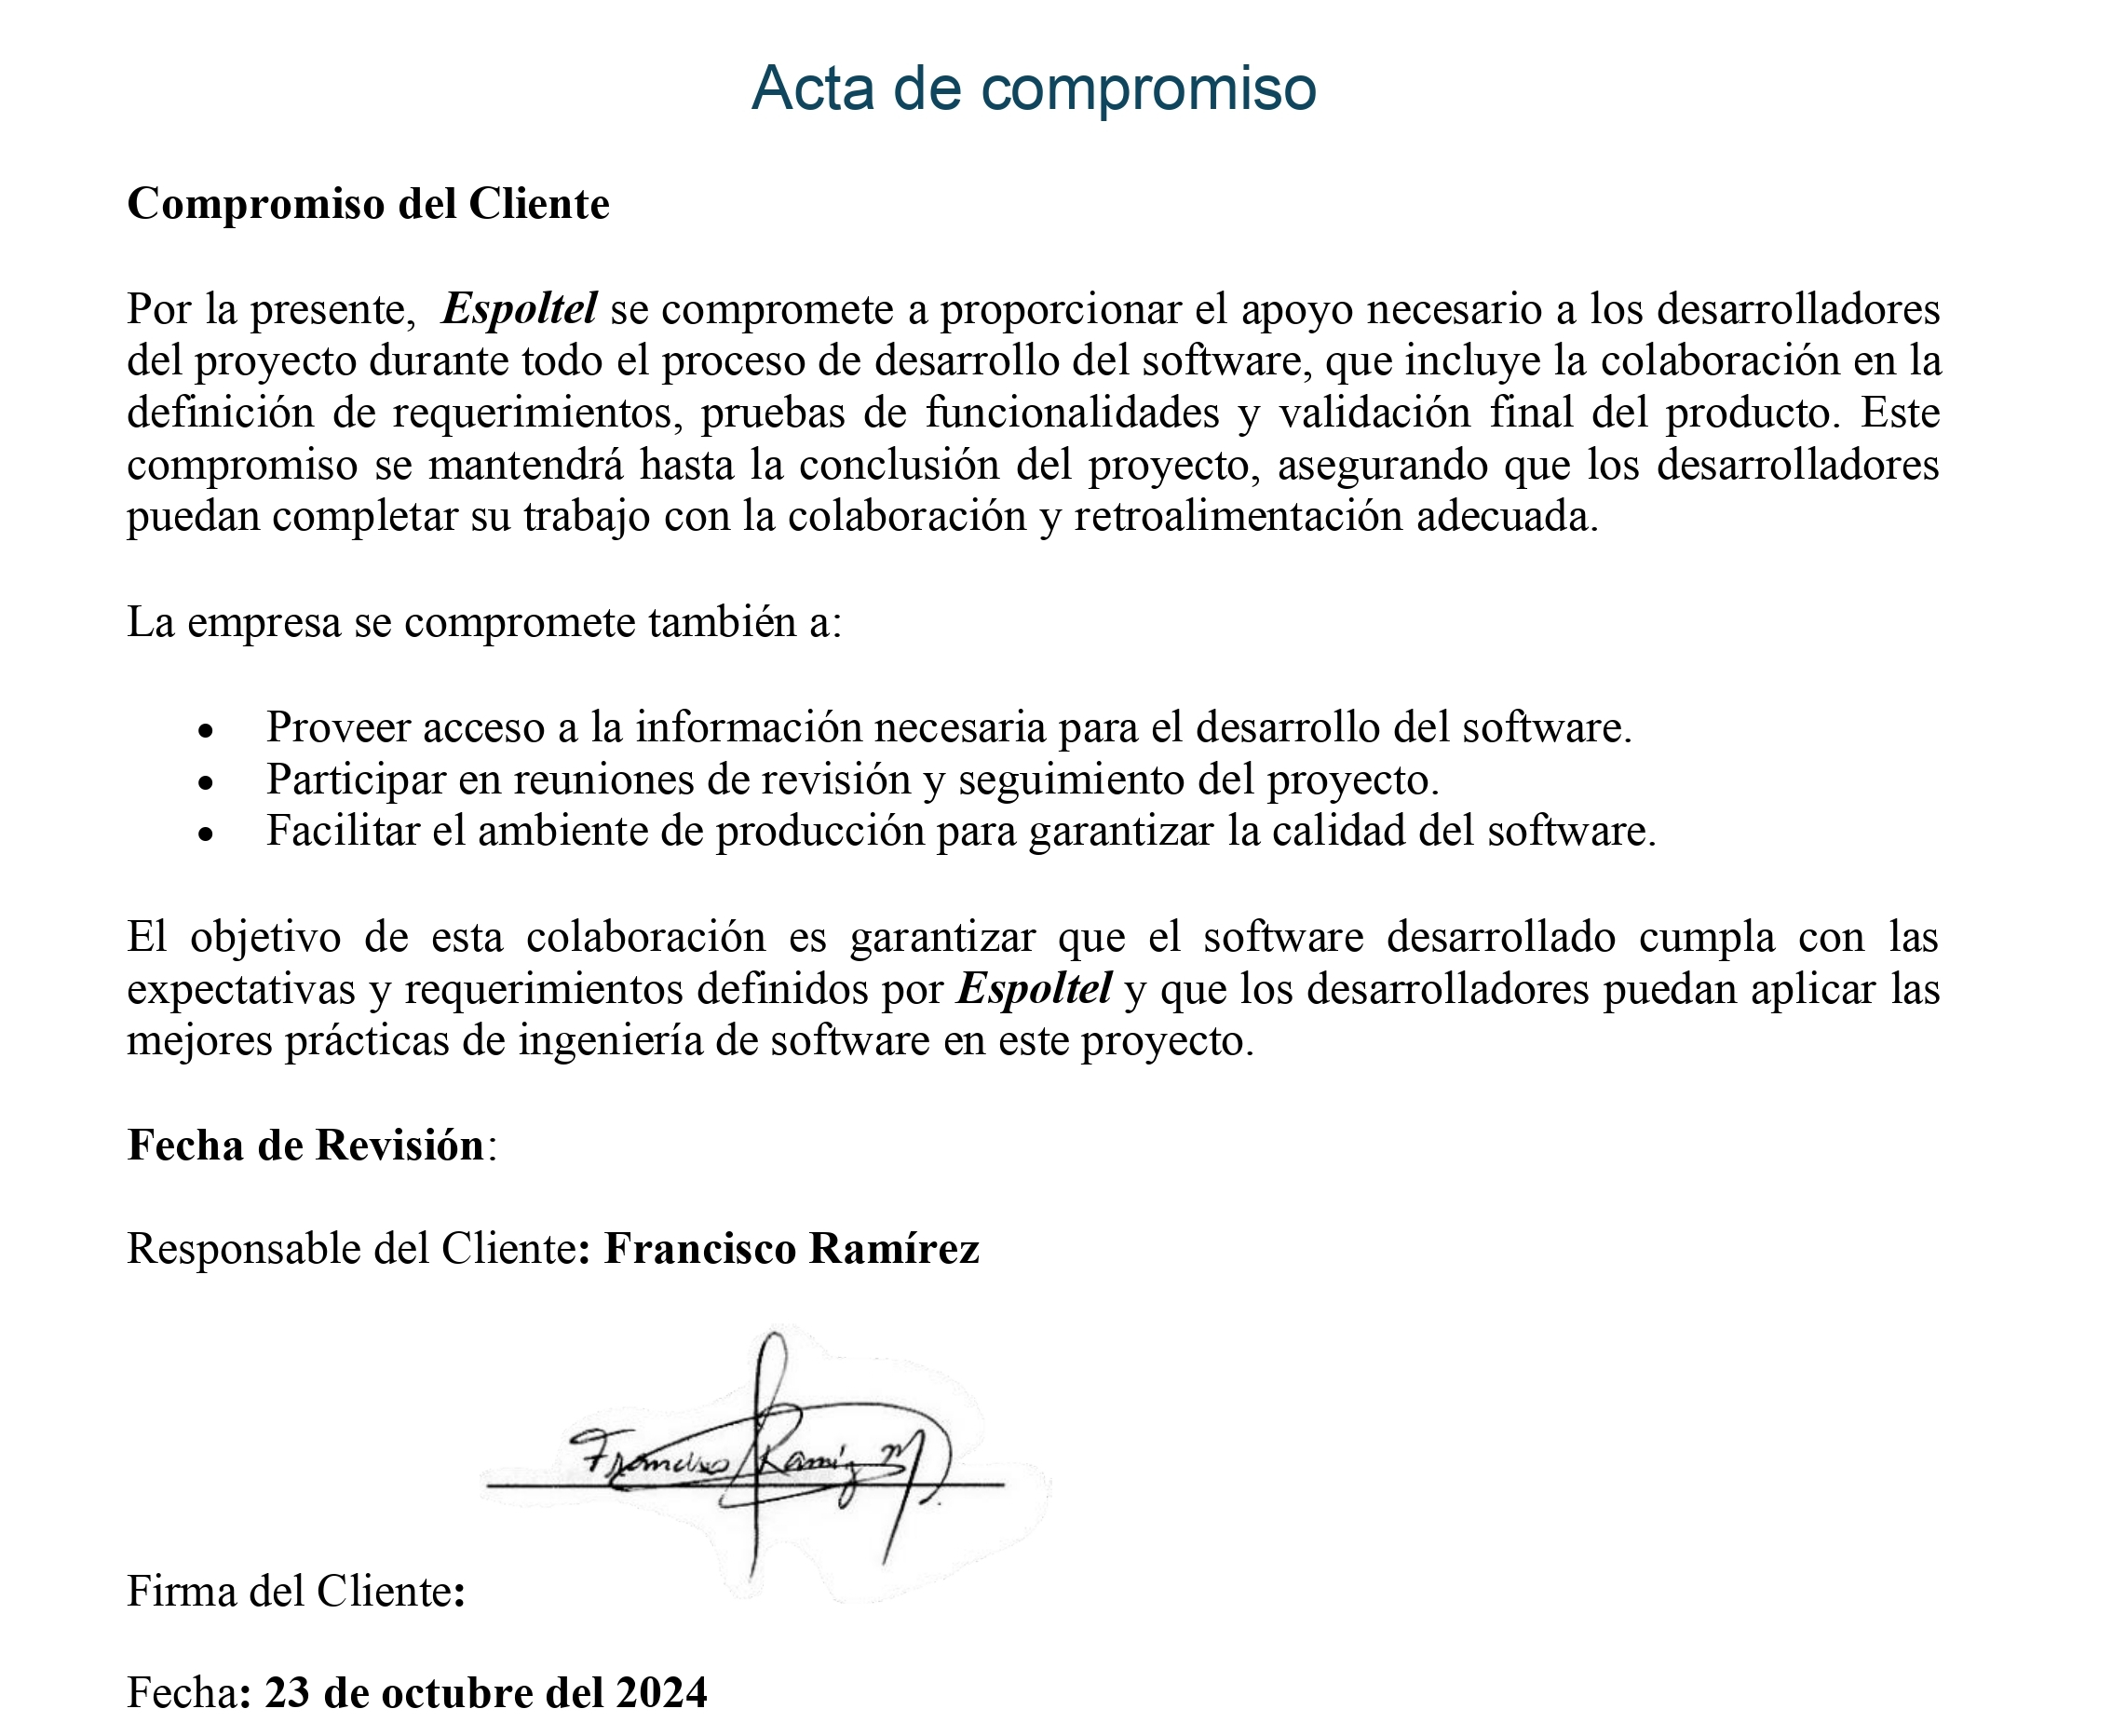
\includegraphics[width=0.75\textwidth]{CommitmentAgreement.jpg}
    \caption{Commitment agreement signed by the client}
    \end{figure}
\FloatBarrier 

\section{Appendix C: Evidence of requirements gathering}
\href{https://drive.google.com/file/d/1h30RbdVEBx5Qlg8GVXav69ps1Y7cQVRv/view?usp=drive_link}{Initial interview for requirements gathering with the client}
\subsection*{Template Questions for the Interview}

1. Are "Human Talent" and "Human Resources" distinct roles within the company?

    If yes, is the Human Resources area responsible for generating documents such as contracts and confidentiality agreements?\\

    What we understand is as follows:\\
    Human Talent:
    \begin{itemize}
        \item Requests documents and information from applicants.
        \item Verifies that applicants meet the position requirements.
        \item Sends the data of candidates who meet the requirements to Human Resources.
    \end{itemize}
    Human Resources:
    \begin{itemize}
        \item Generates documents such as contracts and confidentiality agreements.
        \item Sends the generated contracts or agreements to the applicant.
        \item Verifies the applicant's signature.
        \item Sends the documents to managers for their signatures.
    \end{itemize}

2. Must the contracts and confidentiality agreements be signed not only by the managers and applicants but also by the project director?\\

3. In addition to requesting basic information such as names, surnames, cell phone numbers, etc., should the Human Talent area request specific documents according to the profile, such as copies of the ID, voting card, etc.?\\

4. Who is responsible for entering the templates of the contracts or confidentiality agreements into the system: Human Talent or Human Resources?\\

5. Should these templates be created directly within the system? If yes, would the data be in plain text, such as names, surnames, ID numbers, and the positions for electronic signatures (of managers, applicants, and possibly project directors)?\\

6. Would the stages of the applicant acceptance process be as follows?
\begin{itemize}
    \item Application for a profile by submitting information (plain text data and documents).
    Waiting for a response from Human Talent to verify if the applicant meets the requirements.
    If the applicant meets the requirements, waiting for the contract and confidentiality agreements to sign, generated by Human Resources.
    \item Signing the documents.
    \item  Waiting for signature validation by Human Resources.
    \item  Waiting for signatures from managers and directors.
    \item Confirmation of participation in the project.
\end{itemize}


\section{Appendix D: Web Application Prototype Screenshots}

\begin{figure}[H]
	\centering \small
	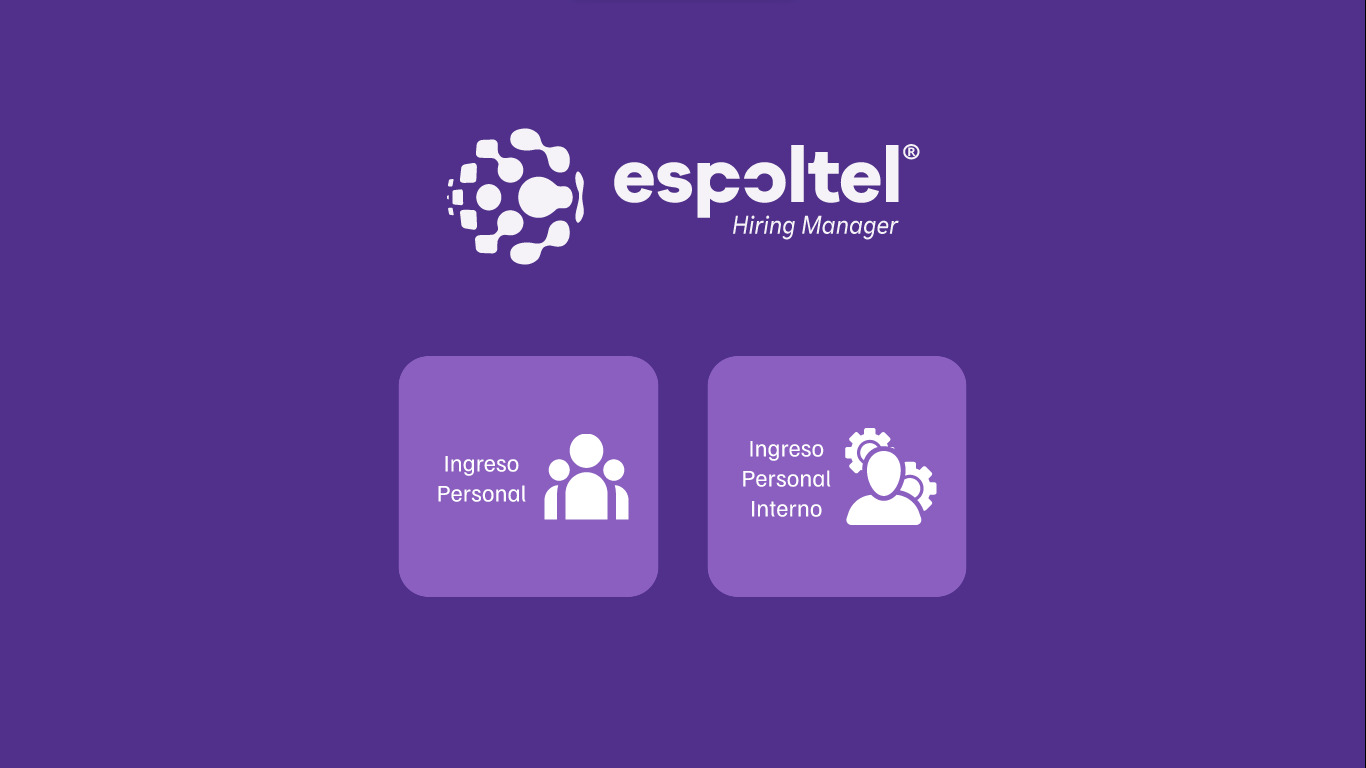
\includegraphics[width=0.8\textwidth]{WebPrototype/wflow-1.jpeg}
	\caption{View of role type selection in ESPOLTEL for authentication}
\end{figure}

\begin{figure}[H]
	\centering \small
	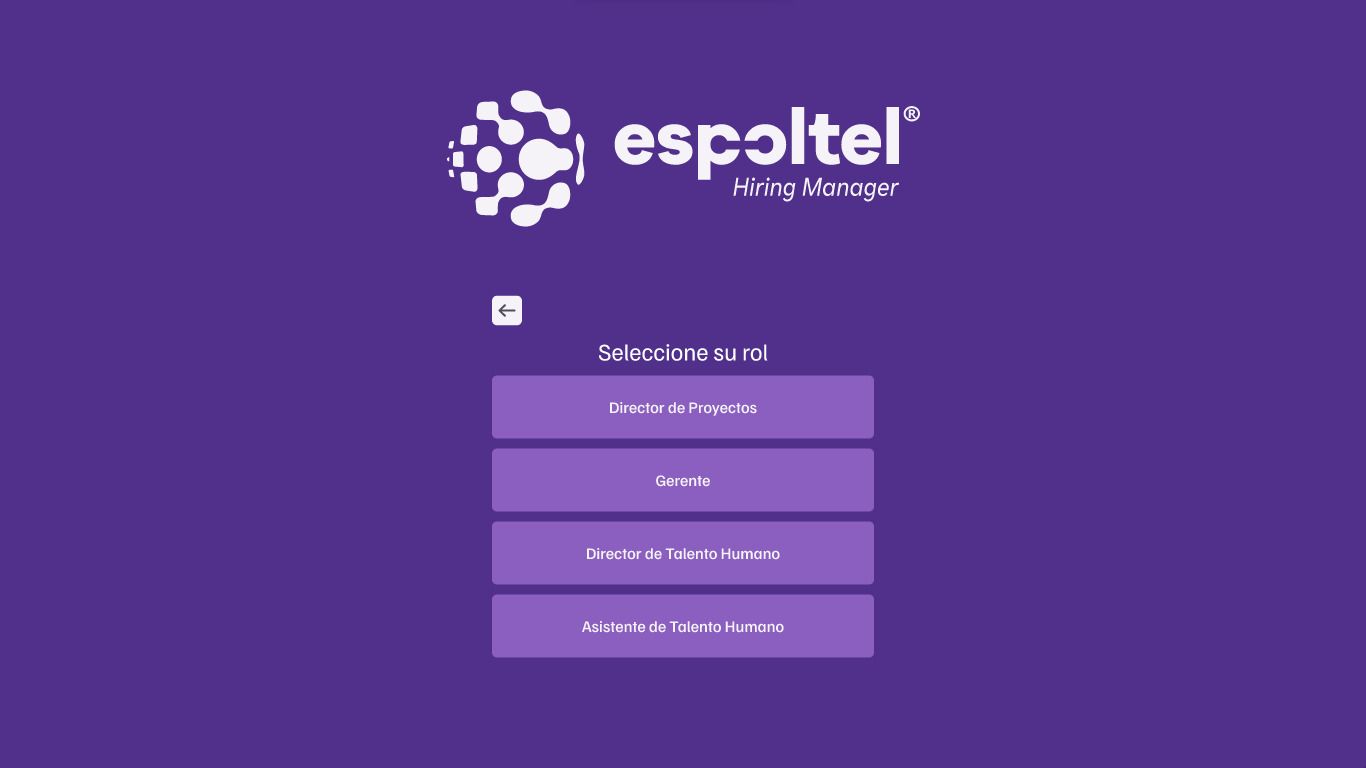
\includegraphics[width=0.8\textwidth]{WebPrototype/wflow-2.jpeg}
	\caption{View of the administrator role selection}
\end{figure}

\begin{figure}[H]
	\centering \small
	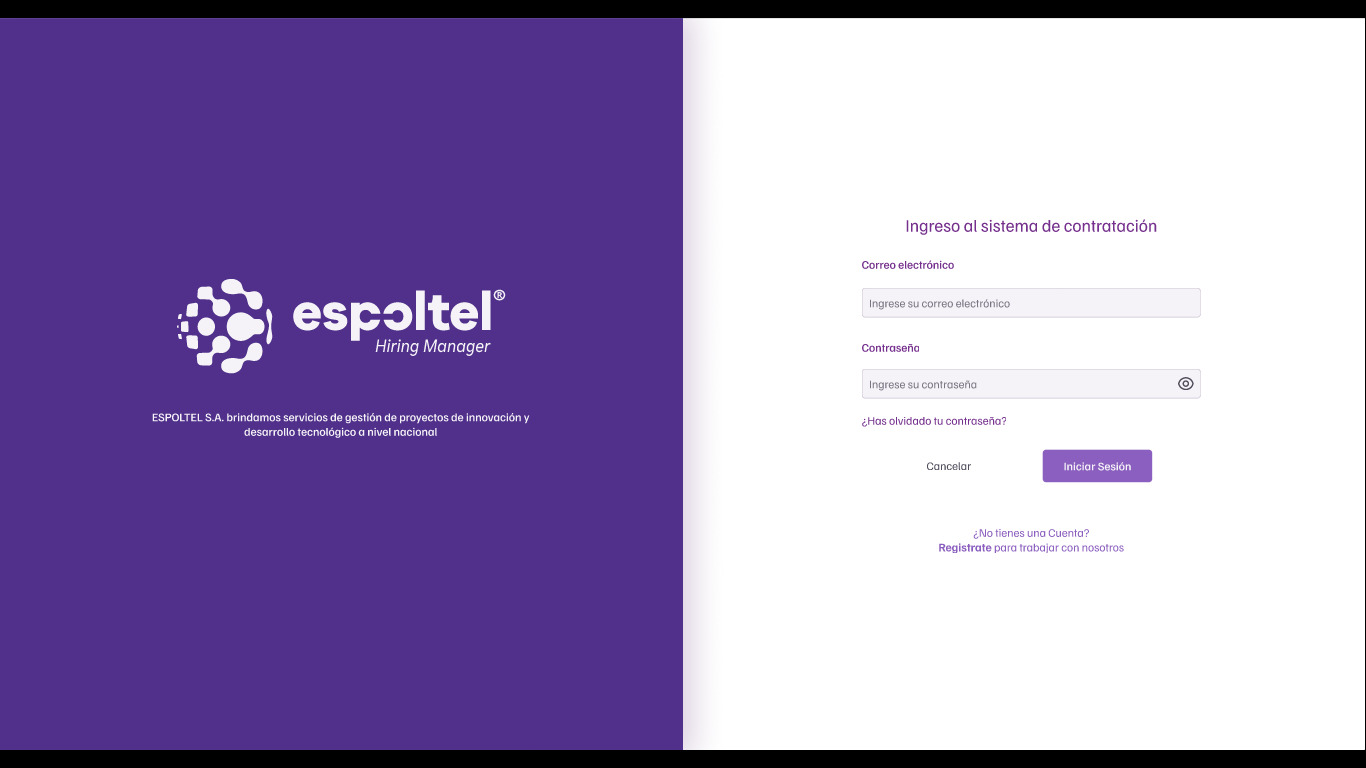
\includegraphics[width=0.8\textwidth]{WebPrototype/wflow-3.jpeg}
	\caption{System login view}
\end{figure}

\begin{figure}[H]
	\centering \small
	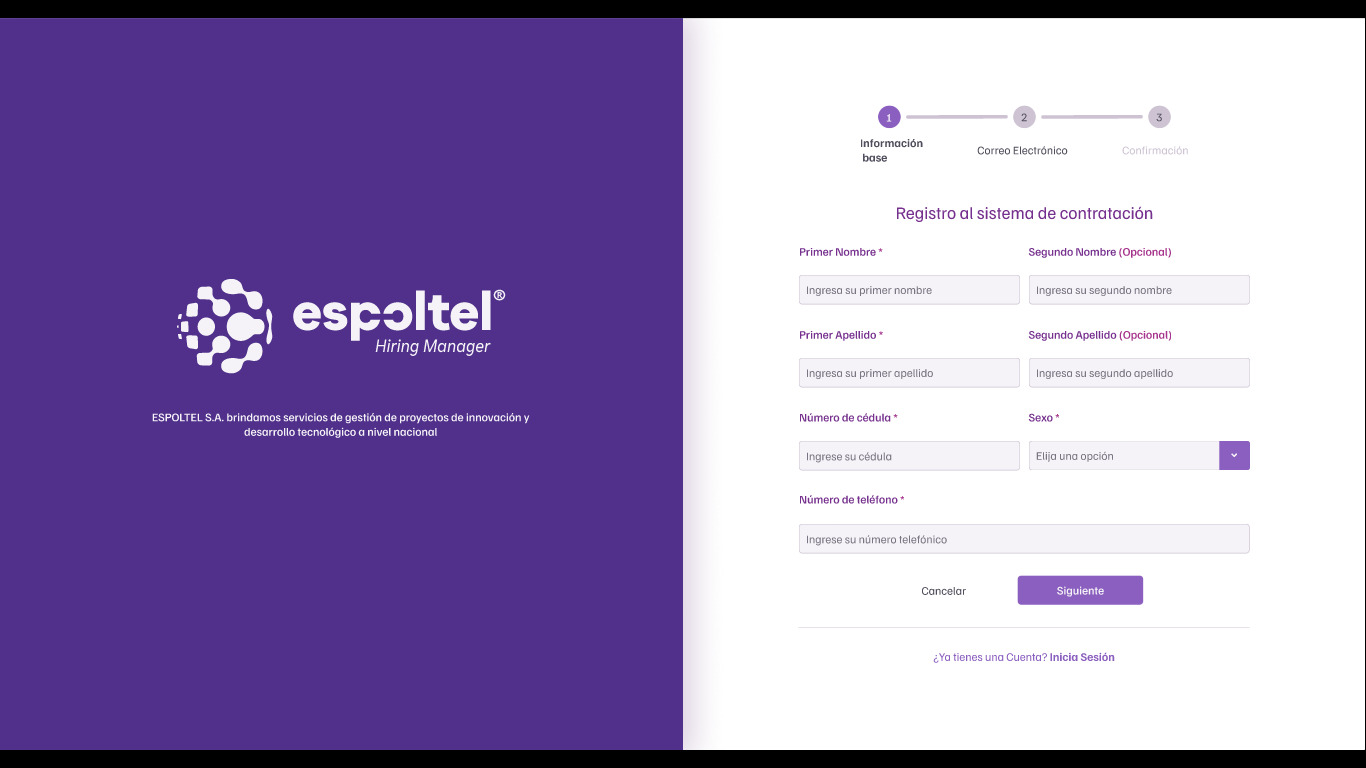
\includegraphics[width=0.8\textwidth]{WebPrototype/wflow-4.jpeg}
	\caption{System registration view, step one: basic information}
\end{figure}

\begin{figure}[H]
	\centering \small
	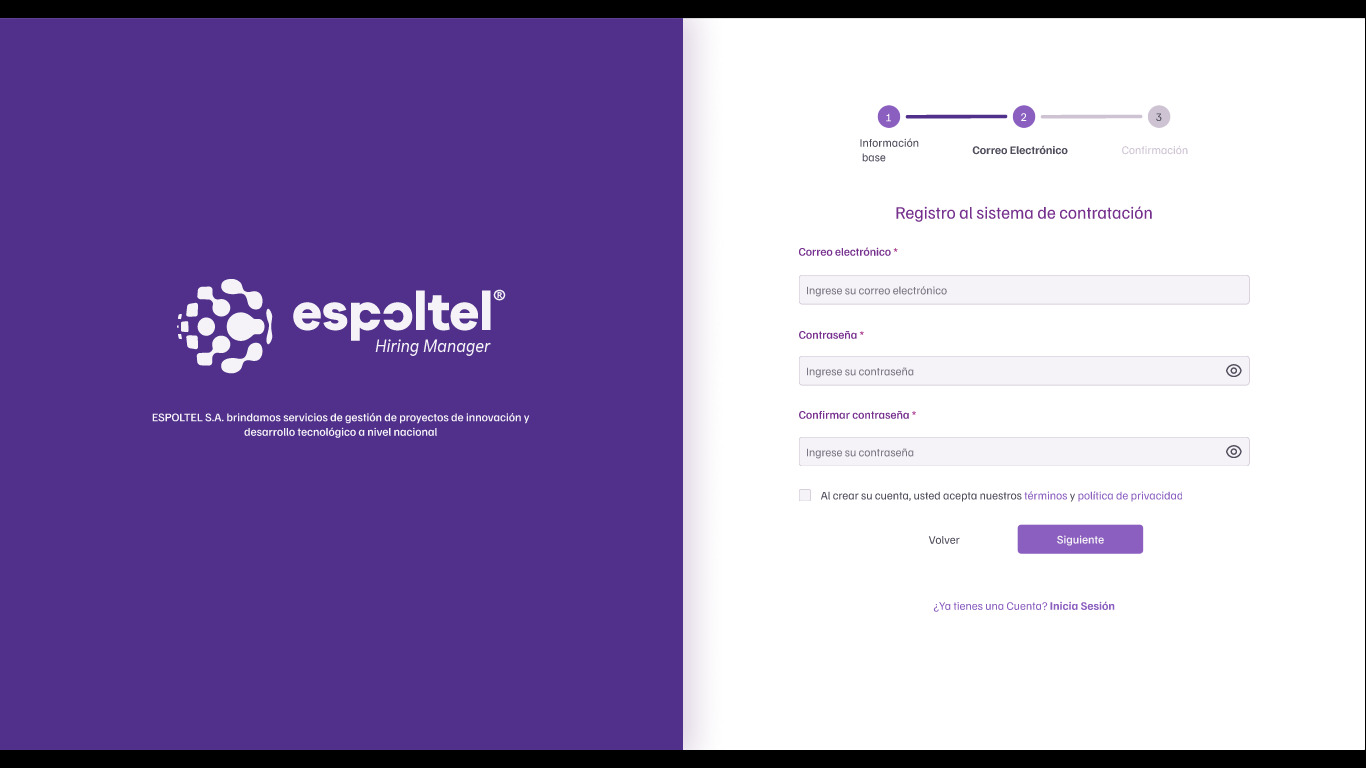
\includegraphics[width=0.8\textwidth]{WebPrototype/wflow-5.jpeg}
	\caption{System registration view, step two: entering email address}
\end{figure}

\begin{figure}[H]
	\centering \small
	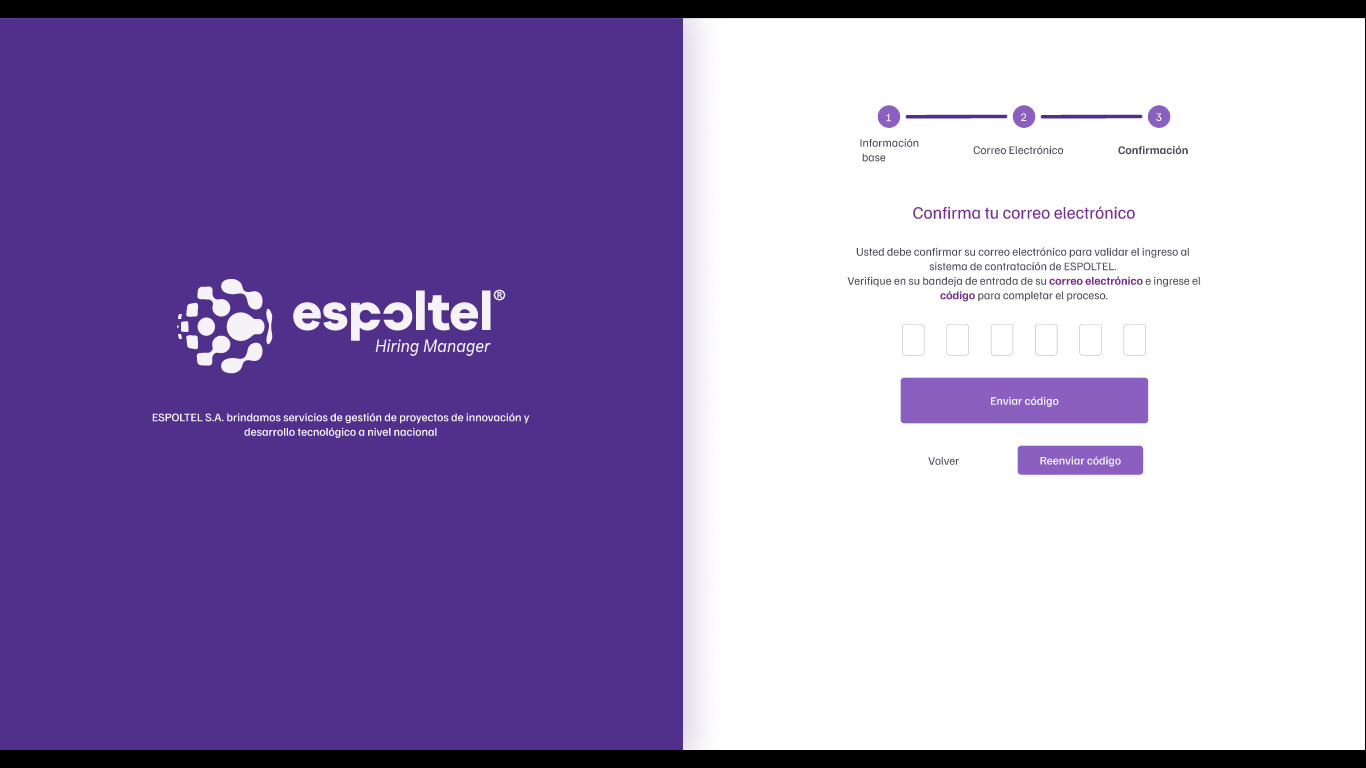
\includegraphics[width=0.8\textwidth]{WebPrototype/wflow-6.jpeg}
	\caption{System registration view, step three: email confirmation }
\end{figure}

\begin{figure}[H]
	\centering \small
	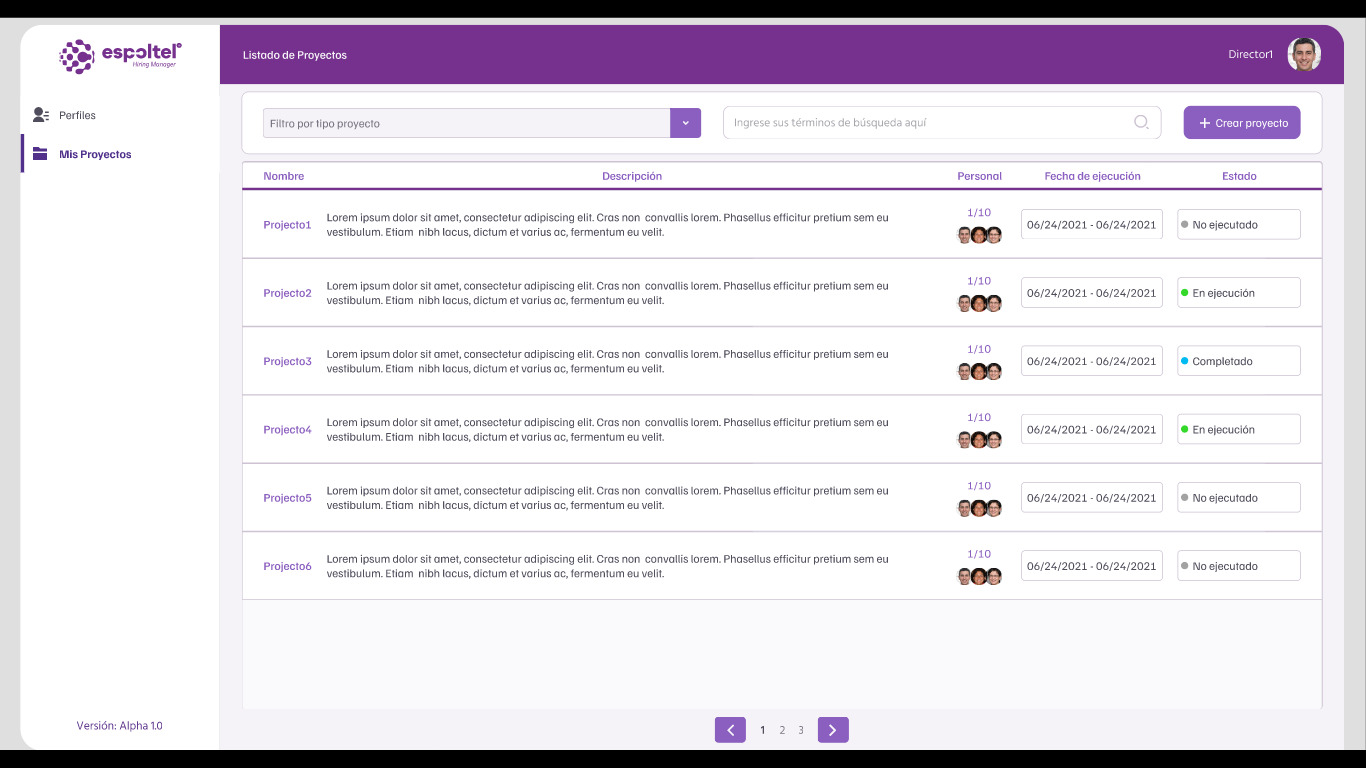
\includegraphics[width=0.8\textwidth]{WebPrototype/wflow-7.jpeg}
	\caption{View of all projects of a director}
\end{figure}

\begin{figure}[H]
	\centering \small
	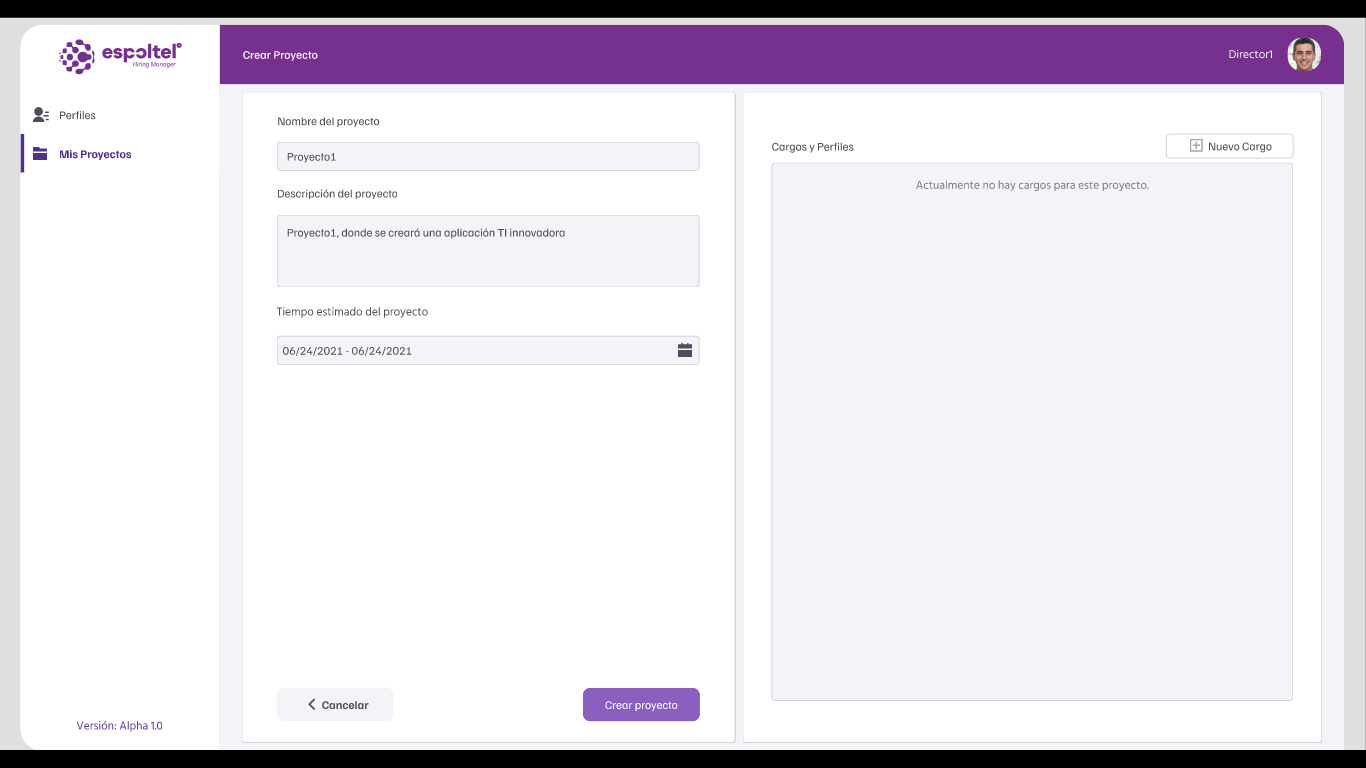
\includegraphics[width=0.8\textwidth]{WebPrototype/wflow-8.jpeg}
	\caption{View of the creation of a project by a director}
\end{figure}

\begin{figure}[H]
	\centering \small
	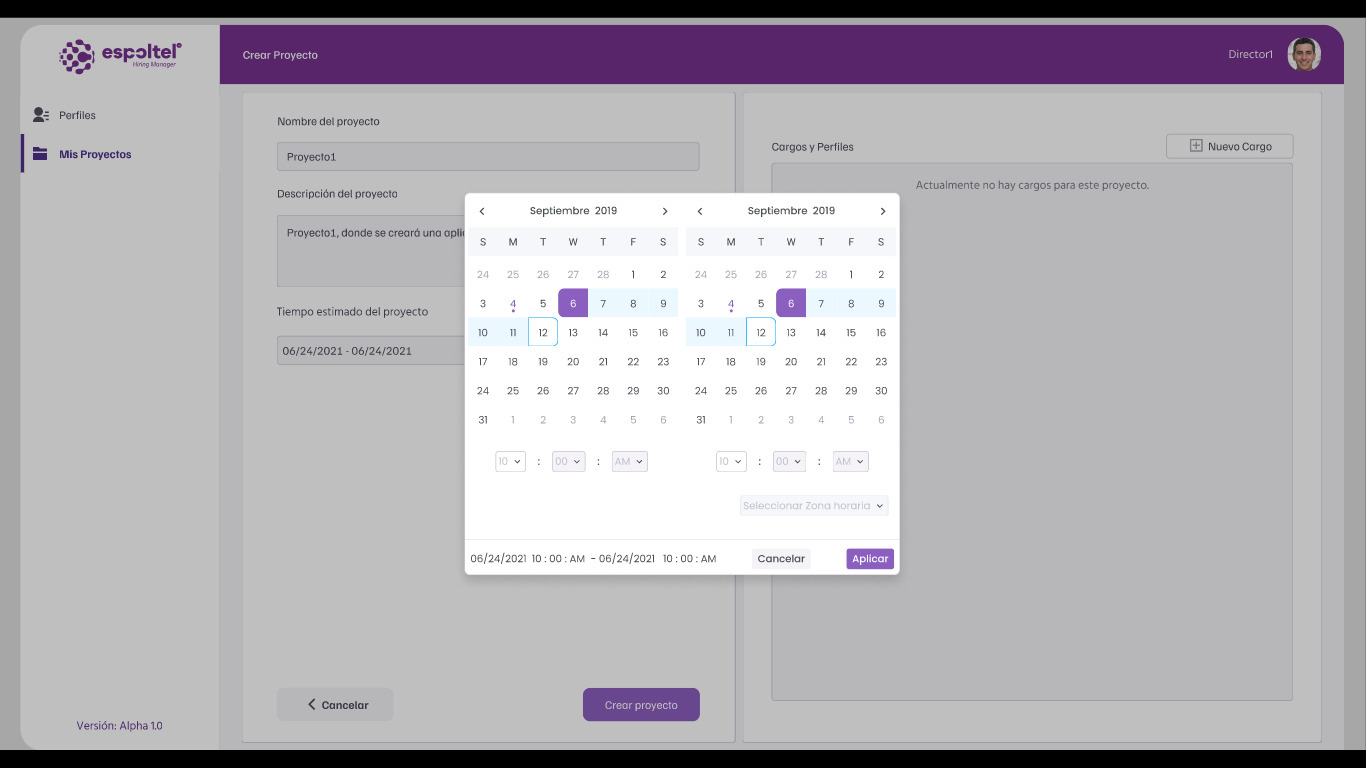
\includegraphics[width=0.8\textwidth]{WebPrototype/wflow-9.jpeg}
	\caption{View of the selection of a project's estimated timeline}
\end{figure}

\begin{figure}[H]
	\centering \small
	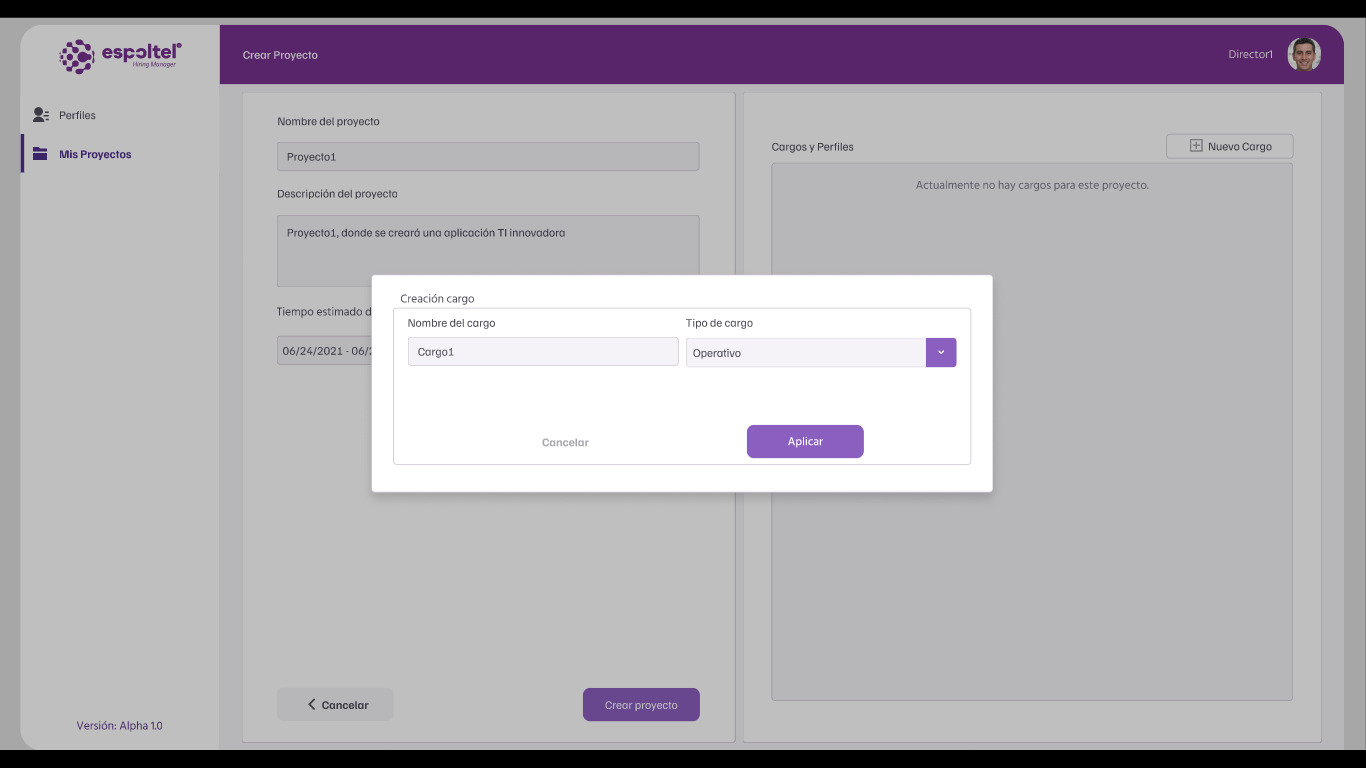
\includegraphics[width=0.8\textwidth]{WebPrototype/wflow-10.jpeg}
	\caption{View of the creation of a project position}
\end{figure}

\begin{figure}[H]
	\centering \small
	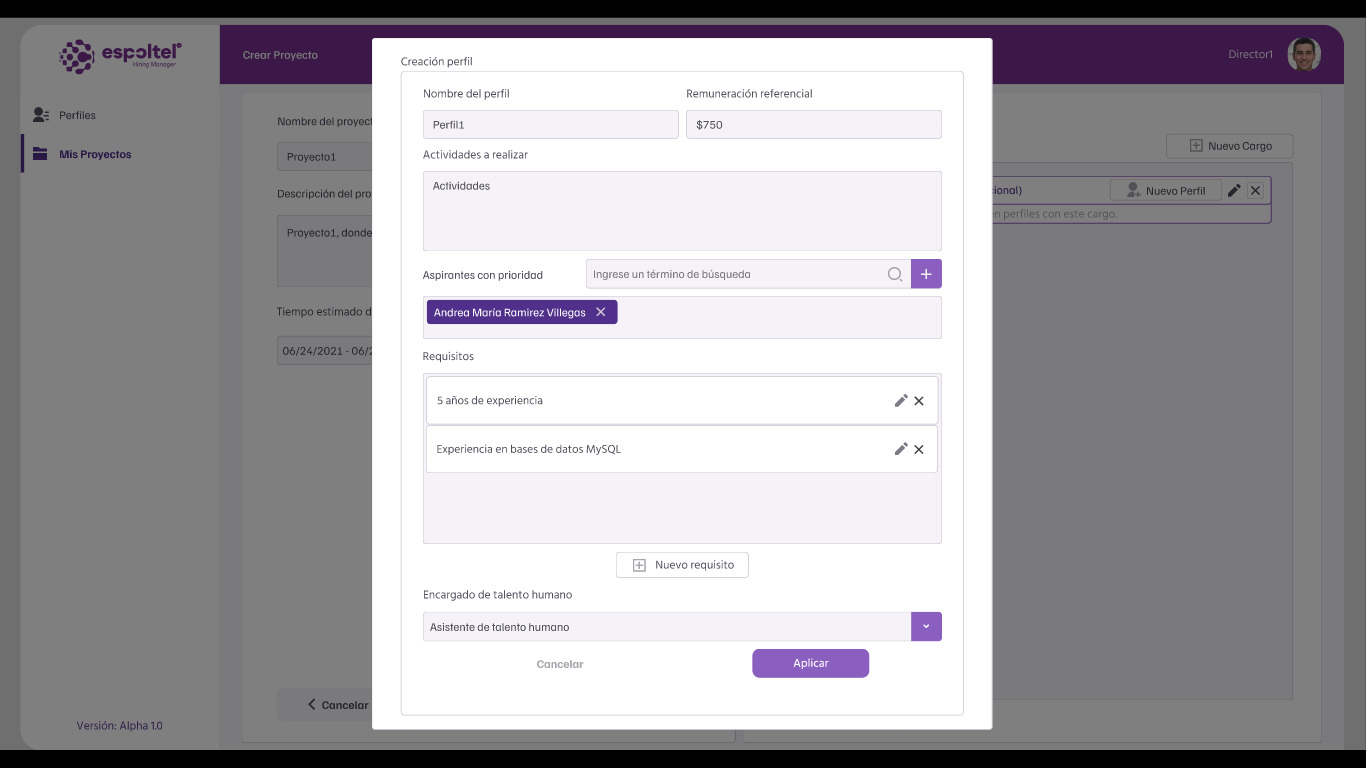
\includegraphics[width=0.8\textwidth]{WebPrototype/wflow-11.jpeg}
	\caption{View of the creation of a project profile}
\end{figure}


\begin{figure}[H]
	\centering \small
	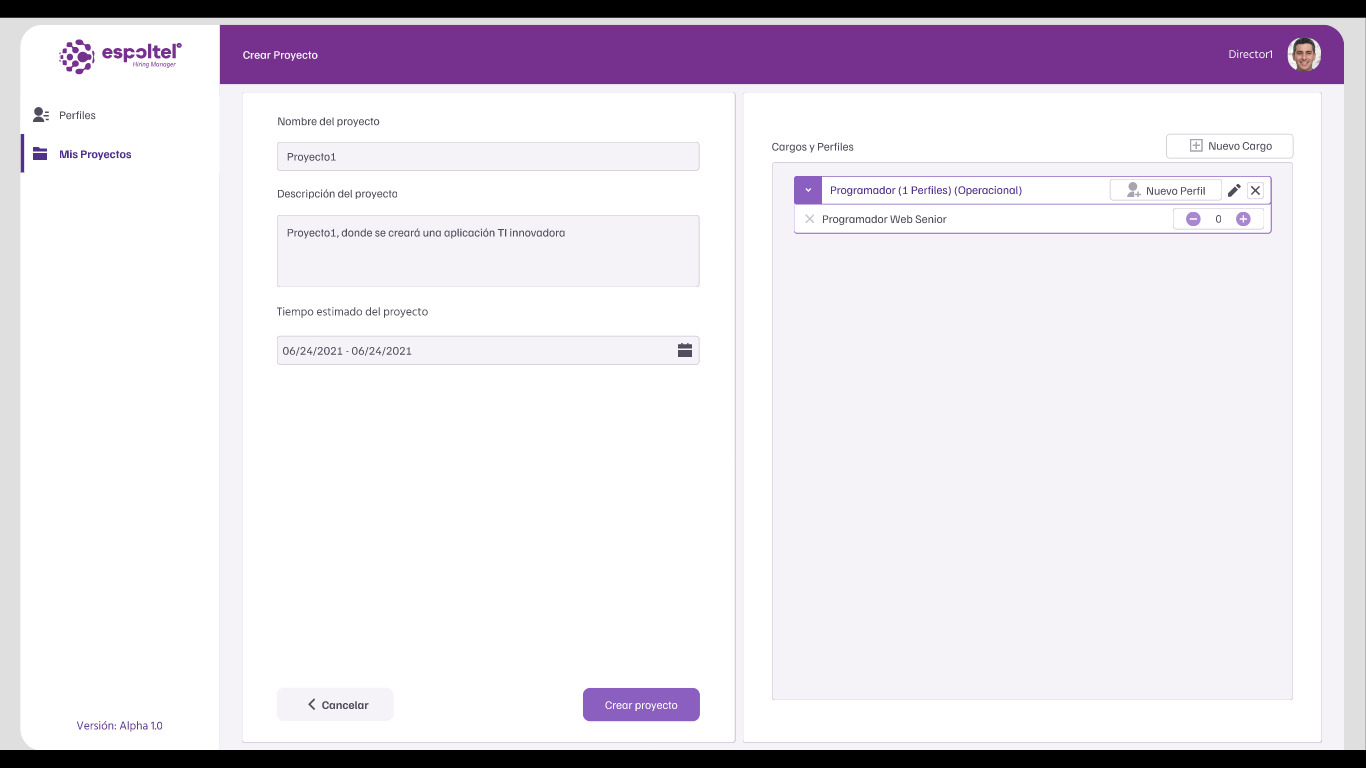
\includegraphics[width=0.8\textwidth]{WebPrototype/wflow-12.jpeg}
	\caption{Project view with roles and profiles}
\end{figure}

\begin{figure}[H]
	\centering \small
	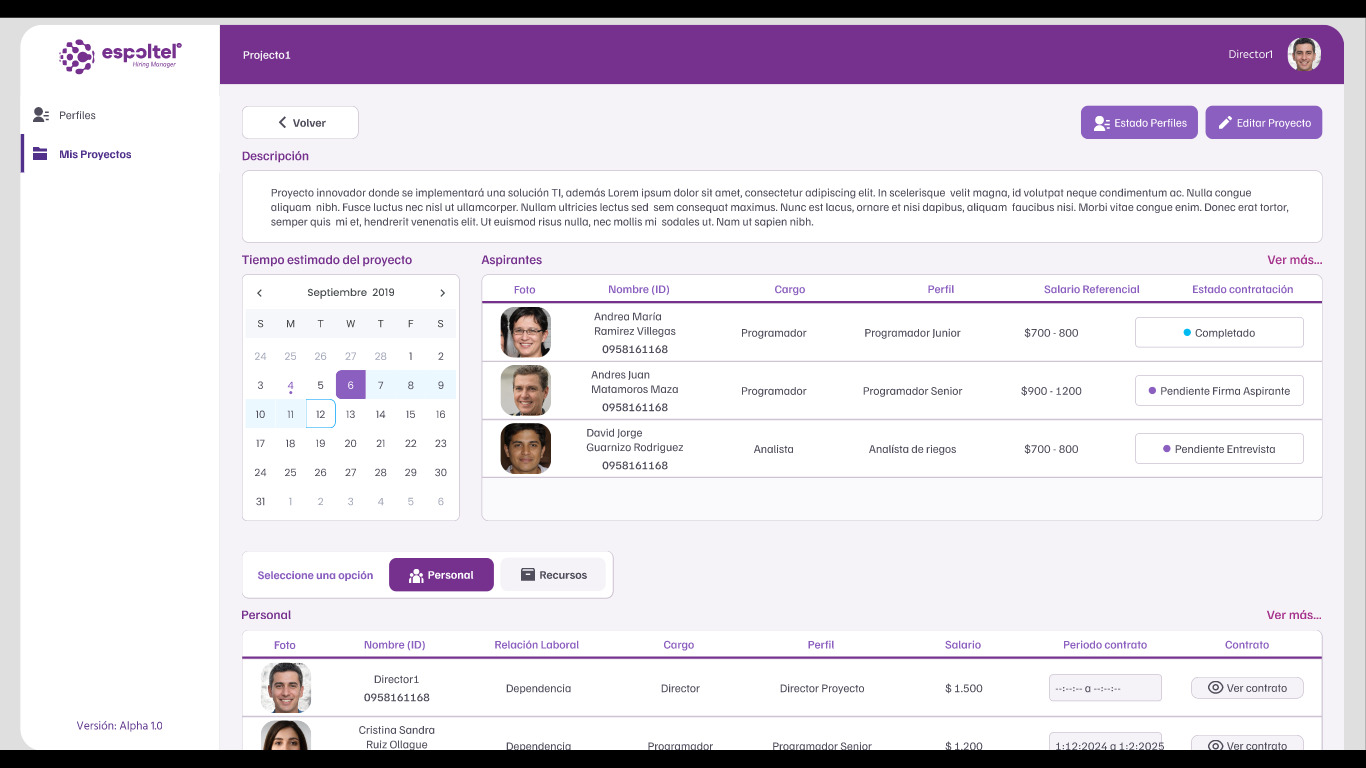
\includegraphics[width=0.8\textwidth]{WebPrototype/wflow-13.jpeg}
	\caption{View of detailed project information}
\end{figure}

\begin{figure}[H]
	\centering \small
	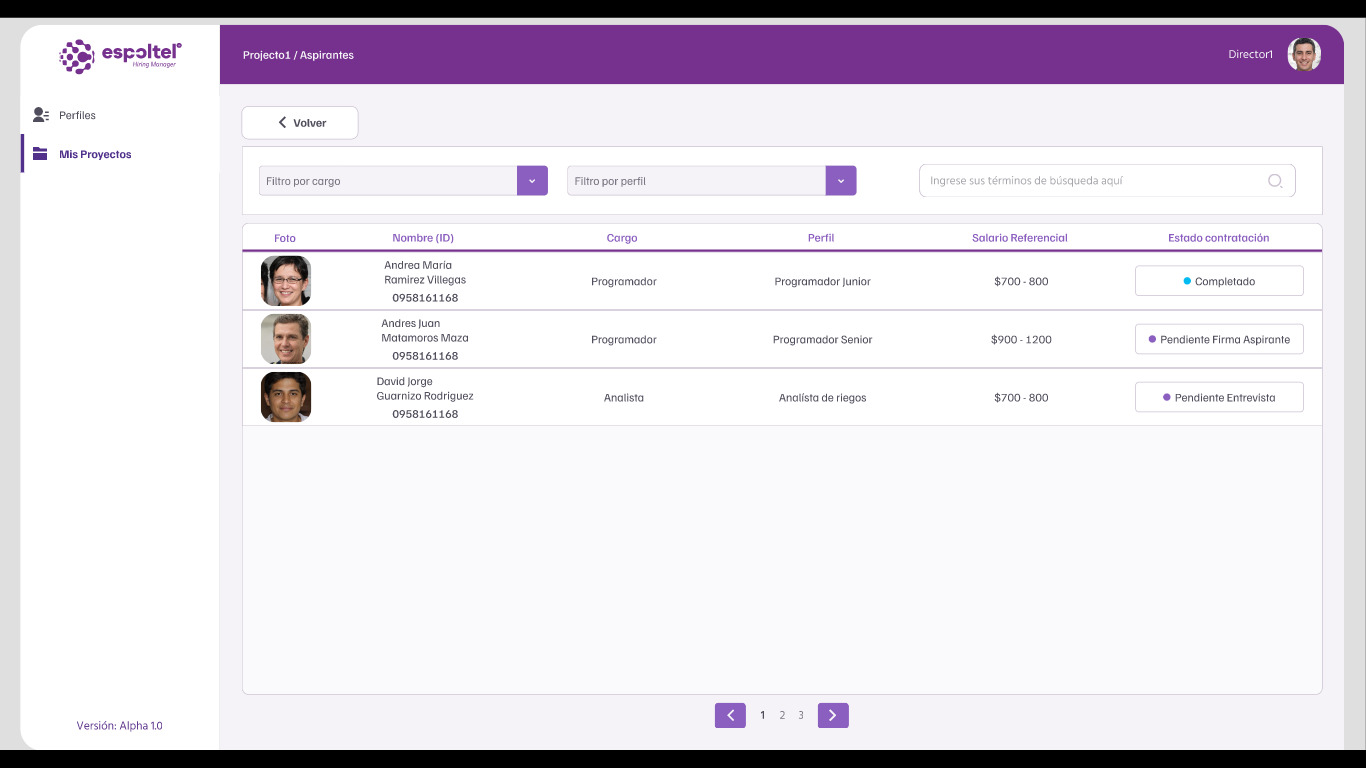
\includegraphics[width=0.8\textwidth]{WebPrototype/wflow-14.jpeg}
	\caption{View of aspirants that have applied for a project}
\end{figure}

\begin{figure}[H]
	\centering \small
	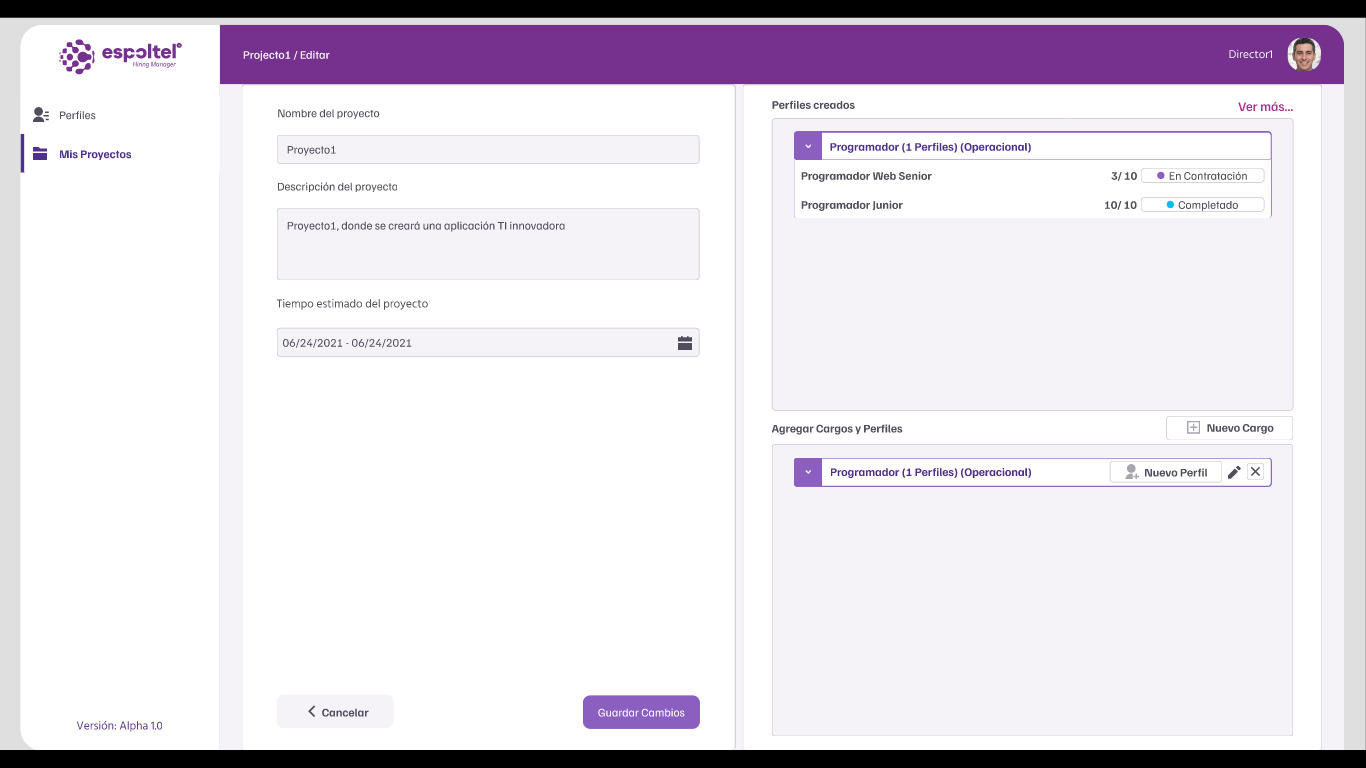
\includegraphics[width=0.8\textwidth]{WebPrototype/wflow-15.jpeg}
	\caption{View of a project edition}
\end{figure}

\begin{figure}[H]
	\centering \small
	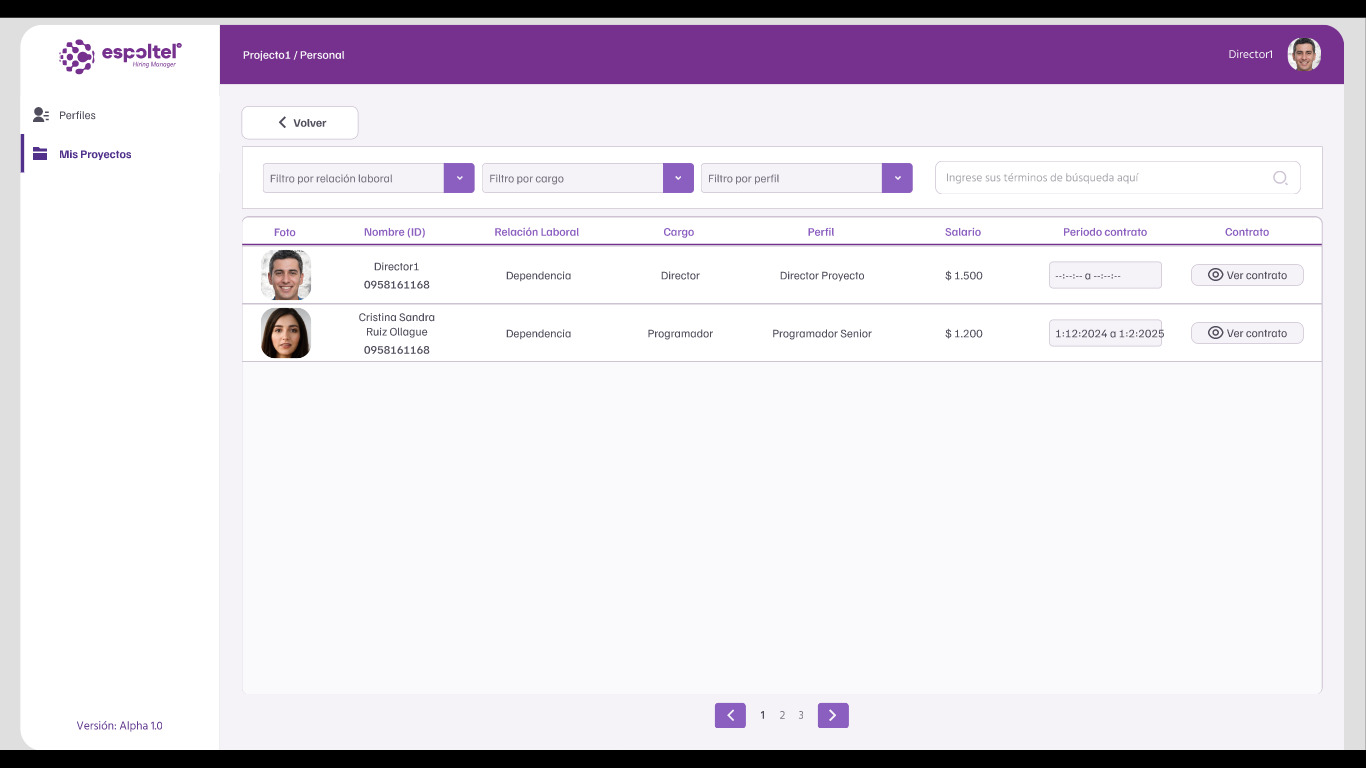
\includegraphics[width=0.8\textwidth]{WebPrototype/wflow-16.jpeg}
	\caption{View of contracted personnel of a project}
\end{figure}

\begin{figure}[H]
	\centering \small
	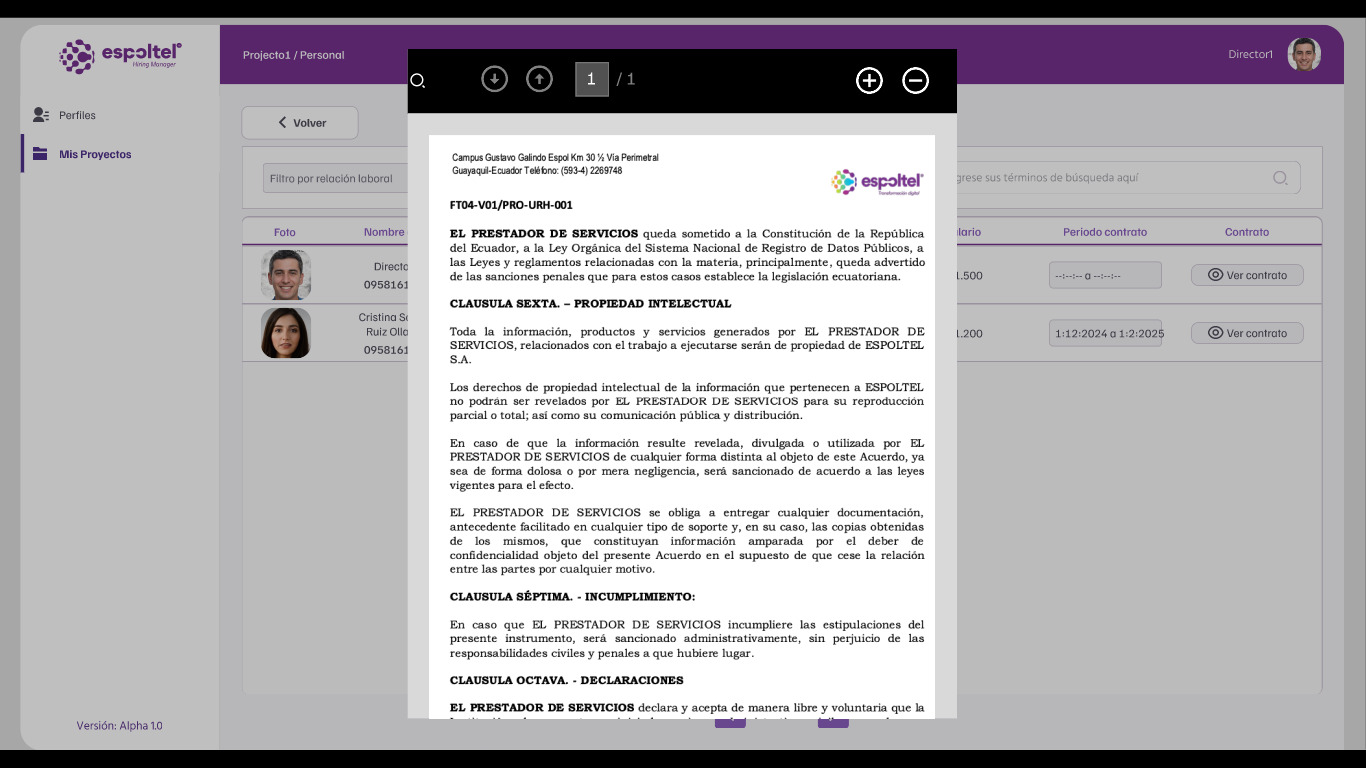
\includegraphics[width=0.8\textwidth]{WebPrototype/wflow-17.jpeg}
	\caption{View of the personnel contract file}
\end{figure}

\begin{figure}[H]
	\centering \small
	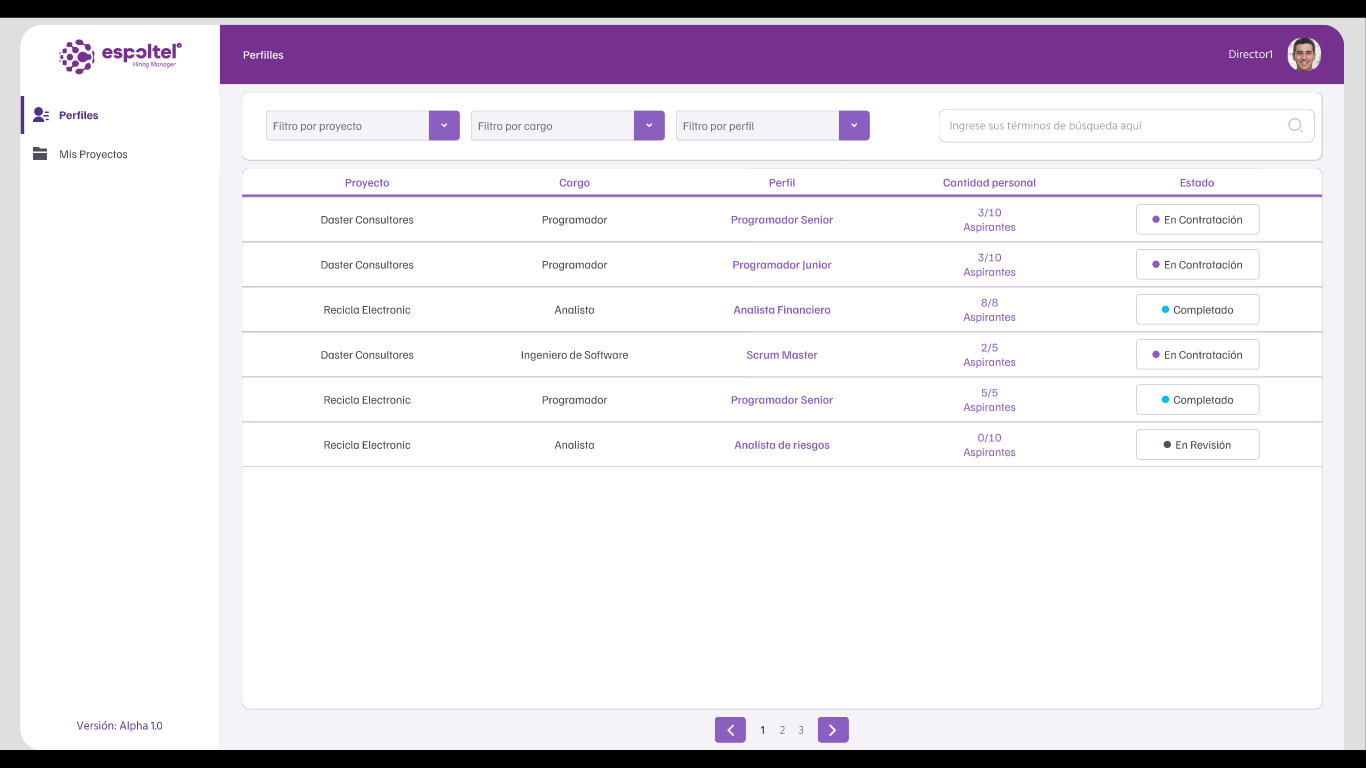
\includegraphics[width=0.8\textwidth]{WebPrototype/wflow-18.jpeg}
	\caption{View of all profiles managed by a director}
\end{figure}

\begin{figure}[H]
	\centering \small
	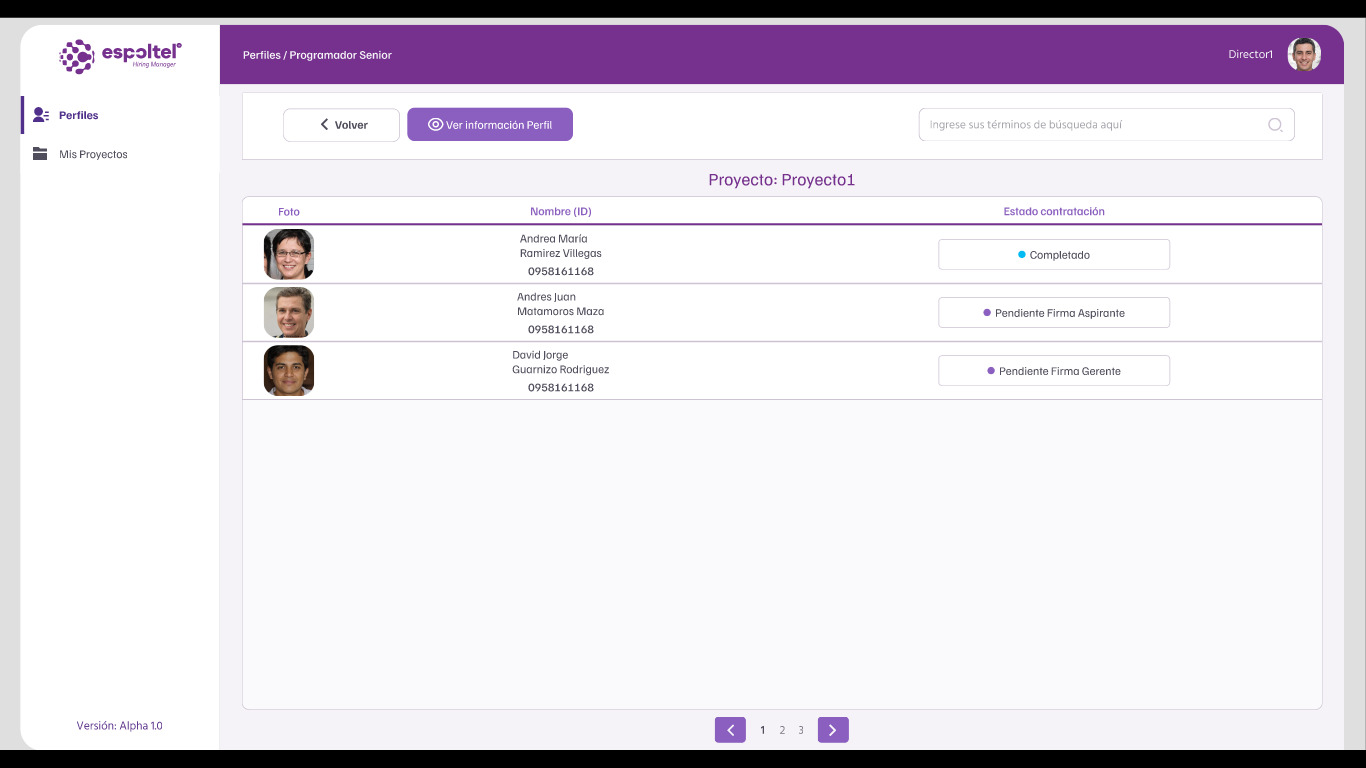
\includegraphics[width=0.8\textwidth]{WebPrototype/wflow-19.jpeg}
	\caption{View of a profile with its postulations in detail}
\end{figure}

\begin{figure}[H]
	\centering \small
	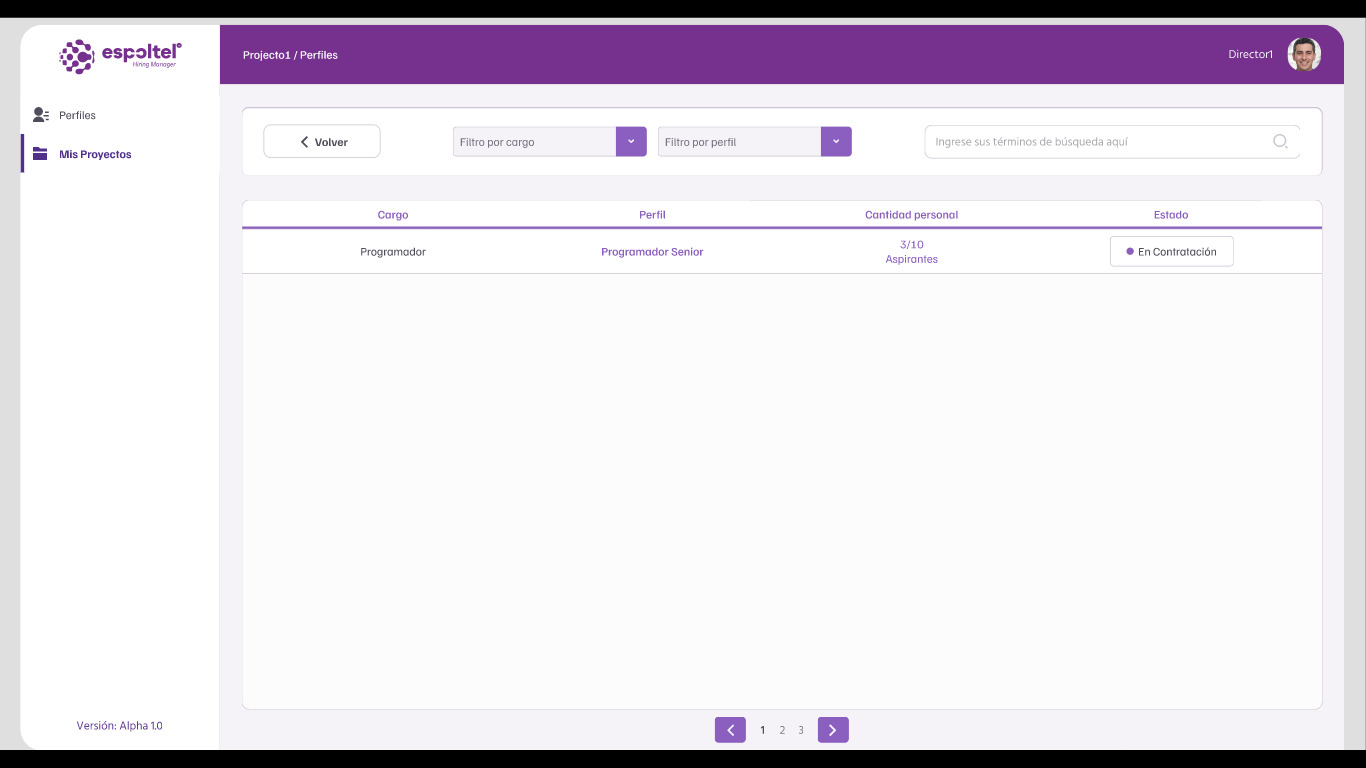
\includegraphics[width=0.8\textwidth]{WebPrototype/wflow-20.jpeg}
	\caption{View of project profiles}
\end{figure}


\begin{figure}[H]
	\centering \small
	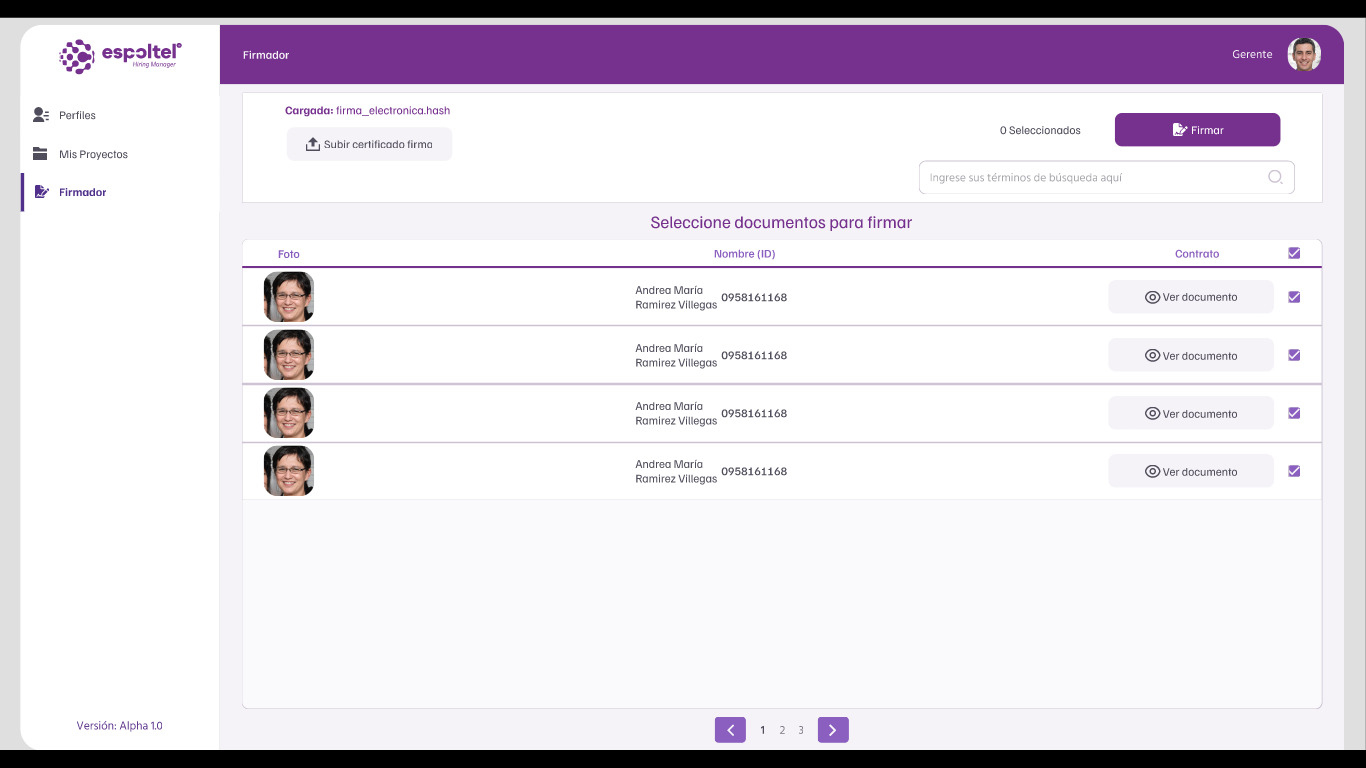
\includegraphics[width=0.8\textwidth]{WebPrototype/wflow-21.jpeg}
	\caption{View of the manager's document signer}
\end{figure}

\begin{figure}[H]
	\centering \small
	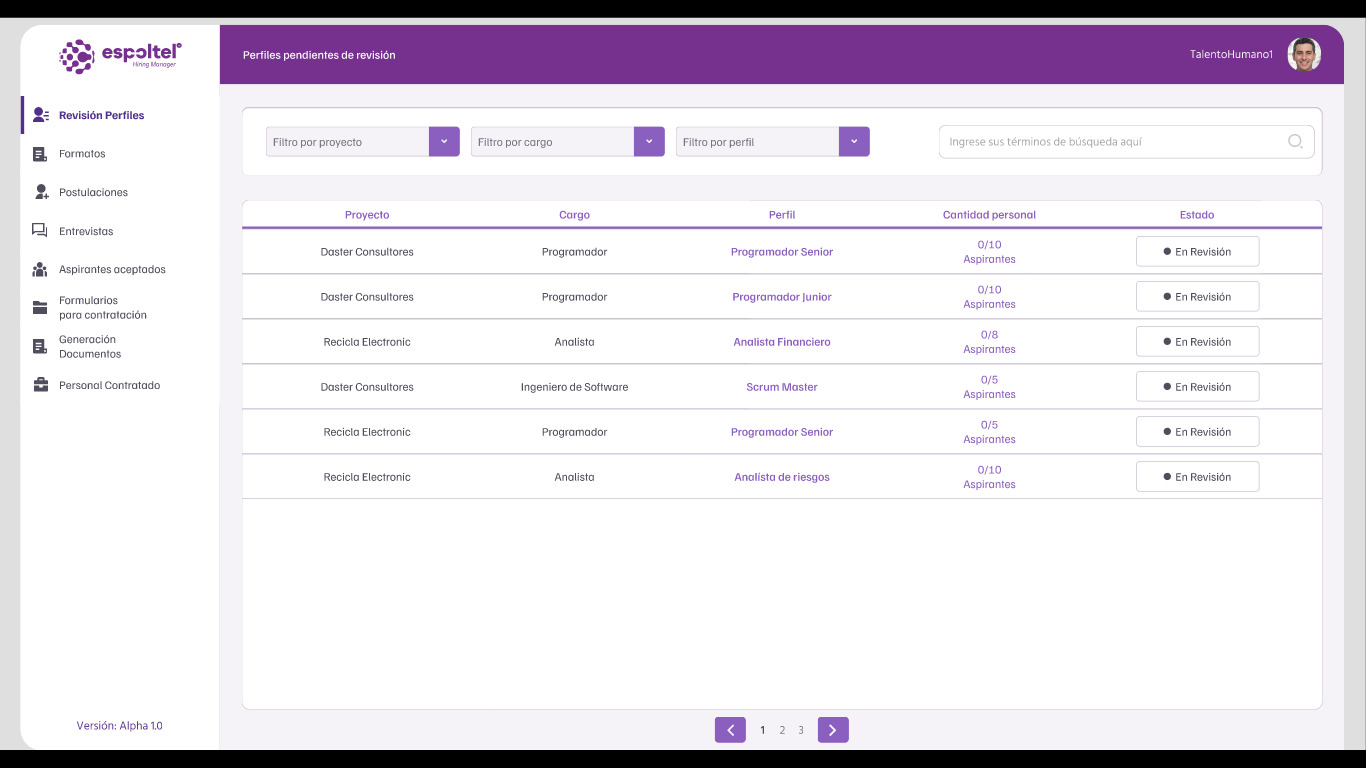
\includegraphics[width=0.8\textwidth]{WebPrototype/wflow-22.jpeg}
	\caption{View of profiles pending review by human talent}
\end{figure}

\begin{figure}[H]
	\centering \small
	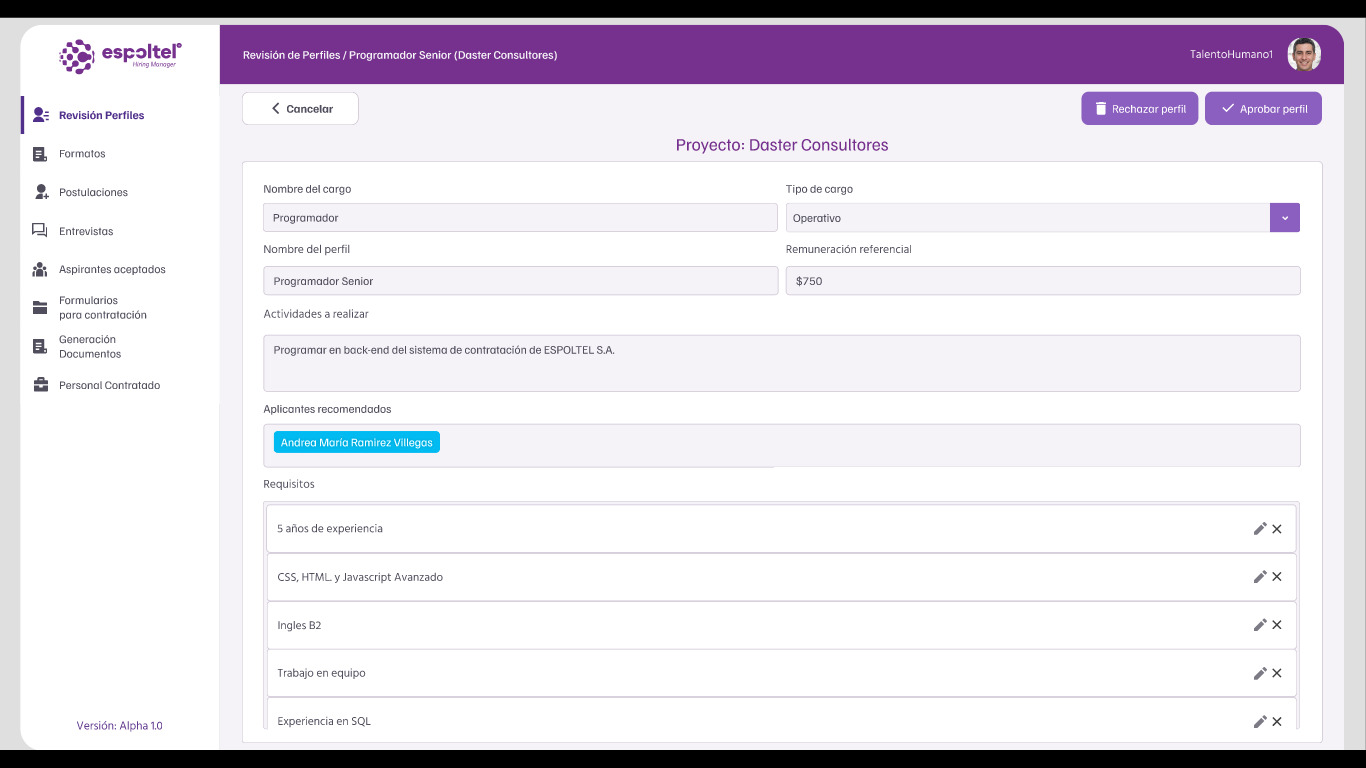
\includegraphics[width=0.8\textwidth]{WebPrototype/wflow-23.jpeg}
	\caption{View a profile revision to edit and accept it}
\end{figure}

\begin{figure}[H]
	\centering \small
	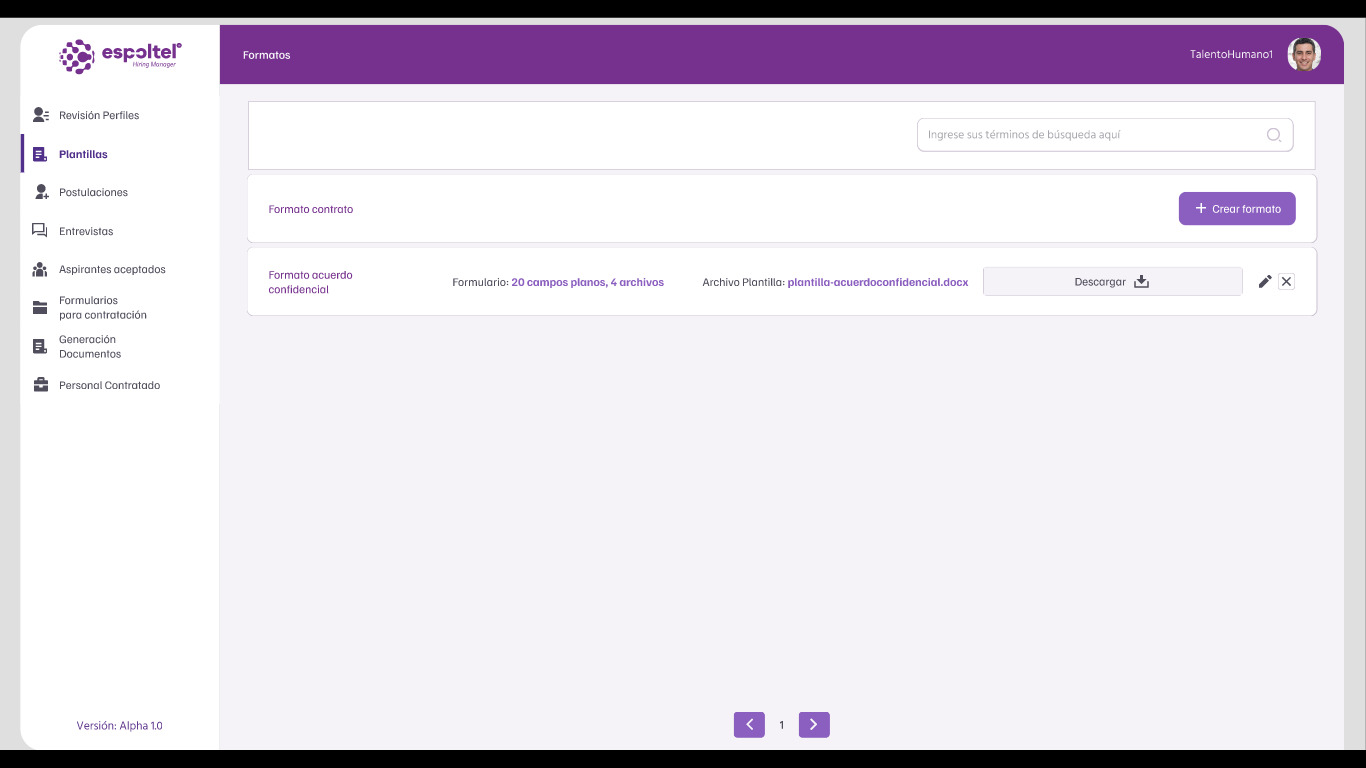
\includegraphics[width=0.8\textwidth]{WebPrototype/wflow-24.jpeg}
	\caption{View of contract and confidential agreement formats}
\end{figure}

\begin{figure}[H]
	\centering \small
	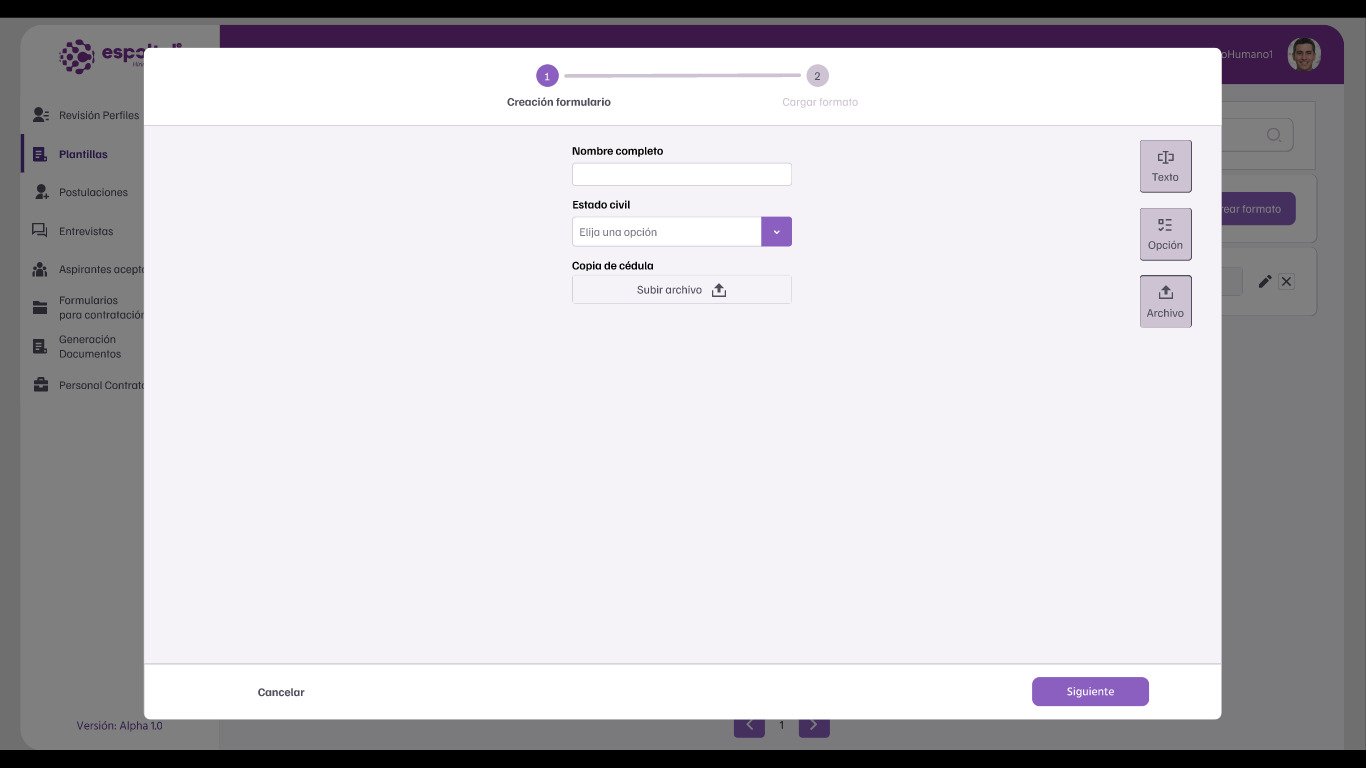
\includegraphics[width=0.8\textwidth]{WebPrototype/wflow-25.jpeg}
	\caption{View of the format creation, step one: create form}
\end{figure}

\begin{figure}[H]
	\centering \small
	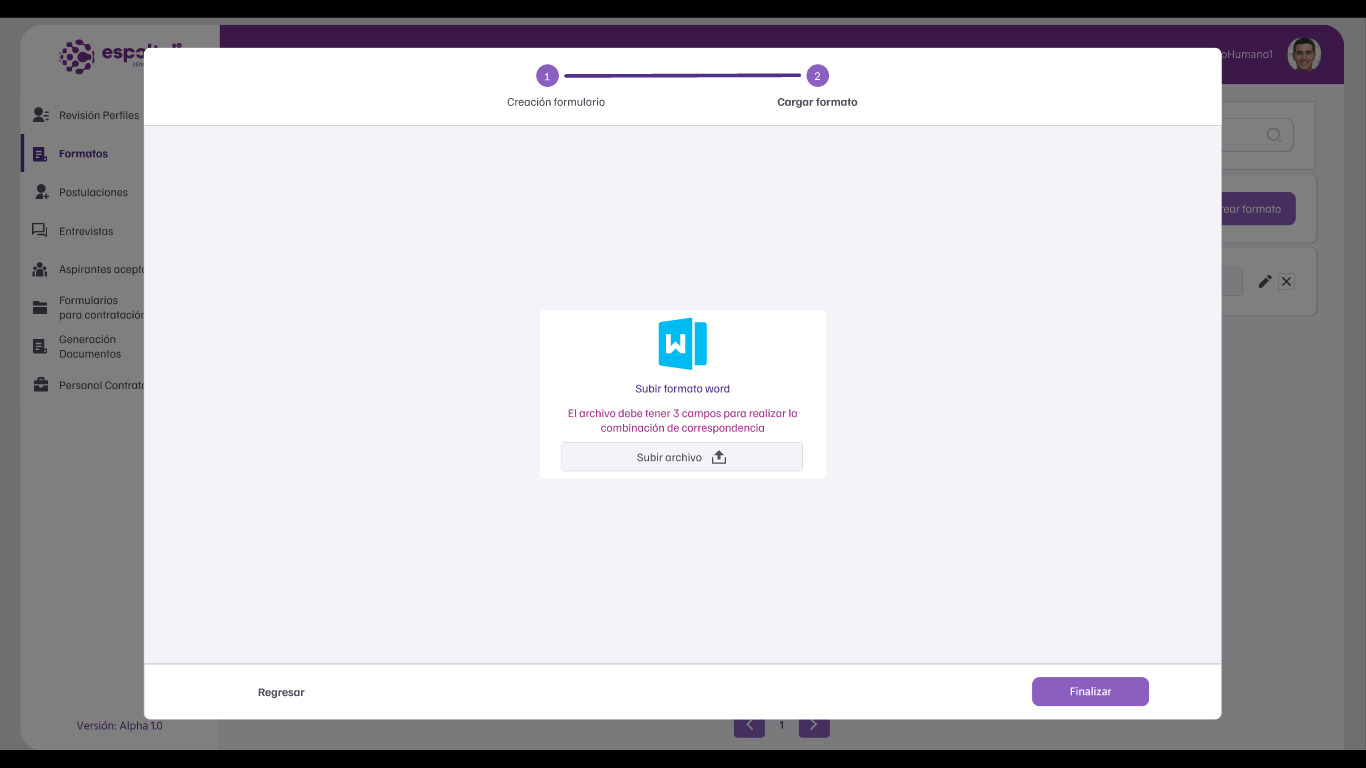
\includegraphics[width=0.8\textwidth]{WebPrototype/wflow-25-2.jpg}
	\caption{View of the format creation, step two: upload the word file}
\end{figure}

\begin{figure}[H]
	\centering \small
	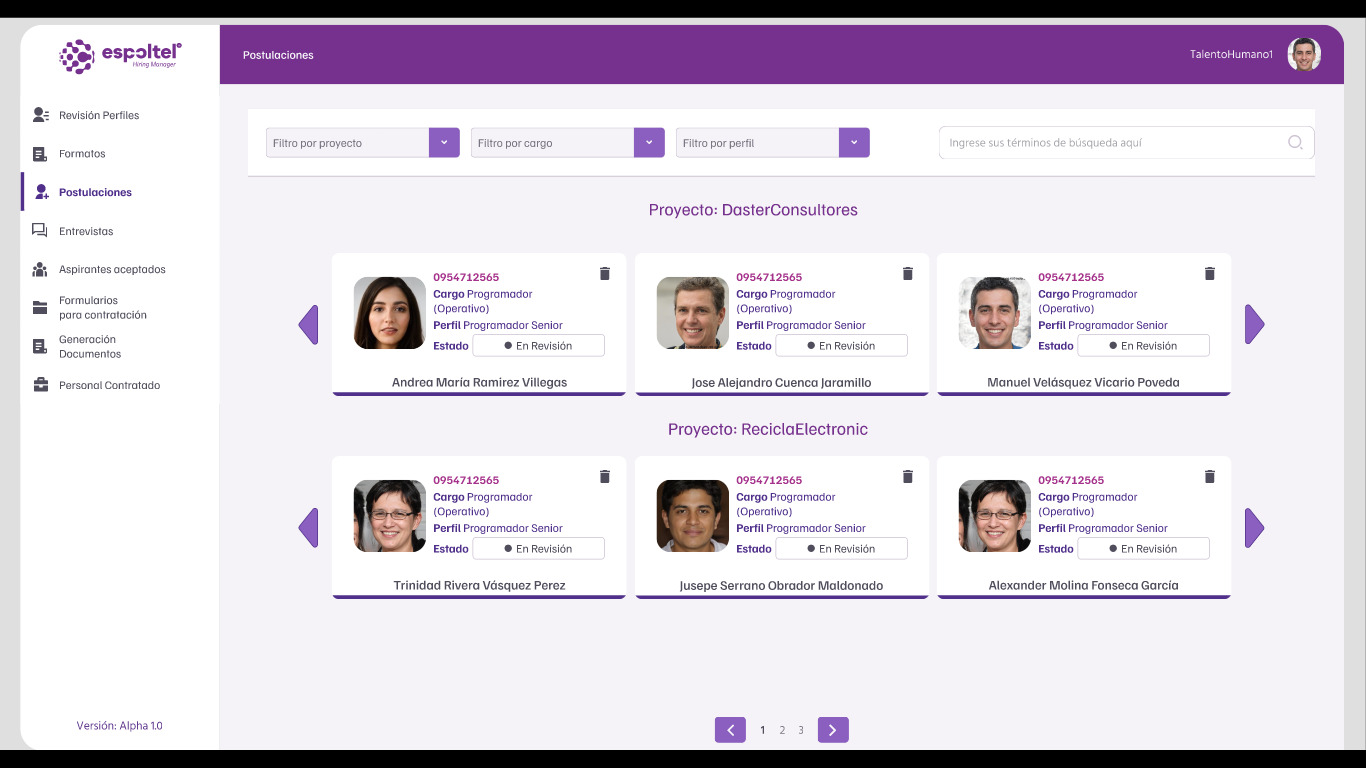
\includegraphics[width=0.8\textwidth]{WebPrototype/wflow-26.jpeg}
	\caption{View of incoming postulations}
\end{figure}

\begin{figure}[H]
	\centering \small
	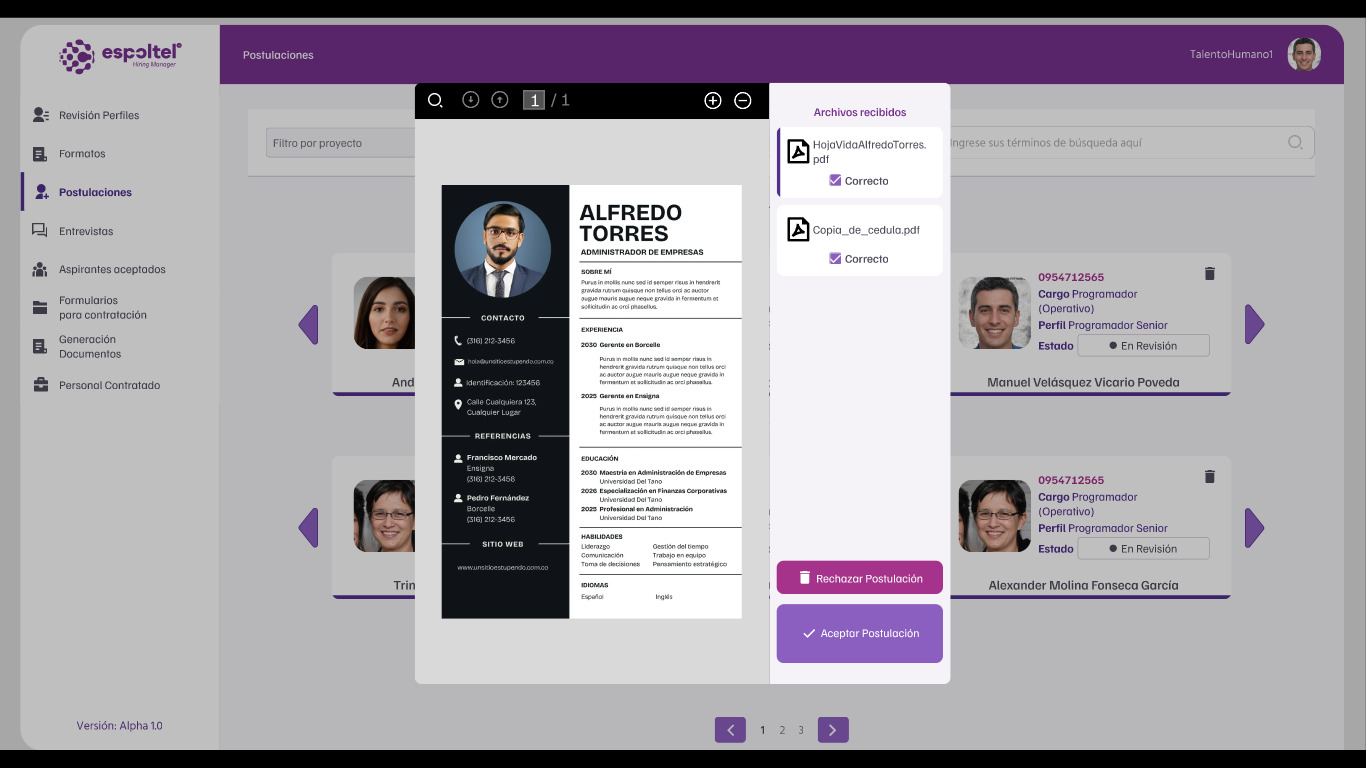
\includegraphics[width=0.8\textwidth]{WebPrototype/wflow-27.jpeg}
	\caption{View validation of documents to accept a postulation under review}
\end{figure}

\begin{figure}[H]
	\centering \small
	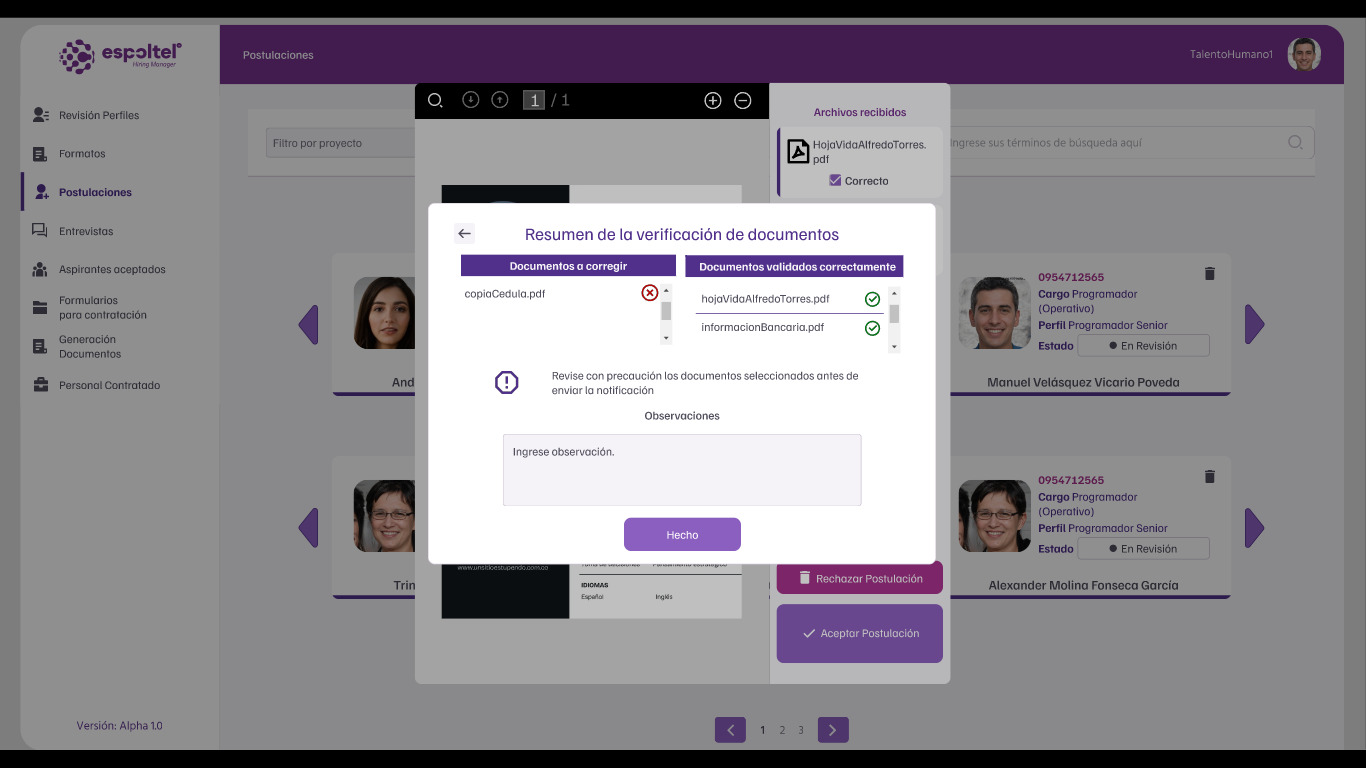
\includegraphics[width=0.8\textwidth]{WebPrototype/wflow-28.jpeg}
	\caption{View of the result of the validation of the postulation to notify the result}
\end{figure}

\begin{figure}[H]
	\centering \small
	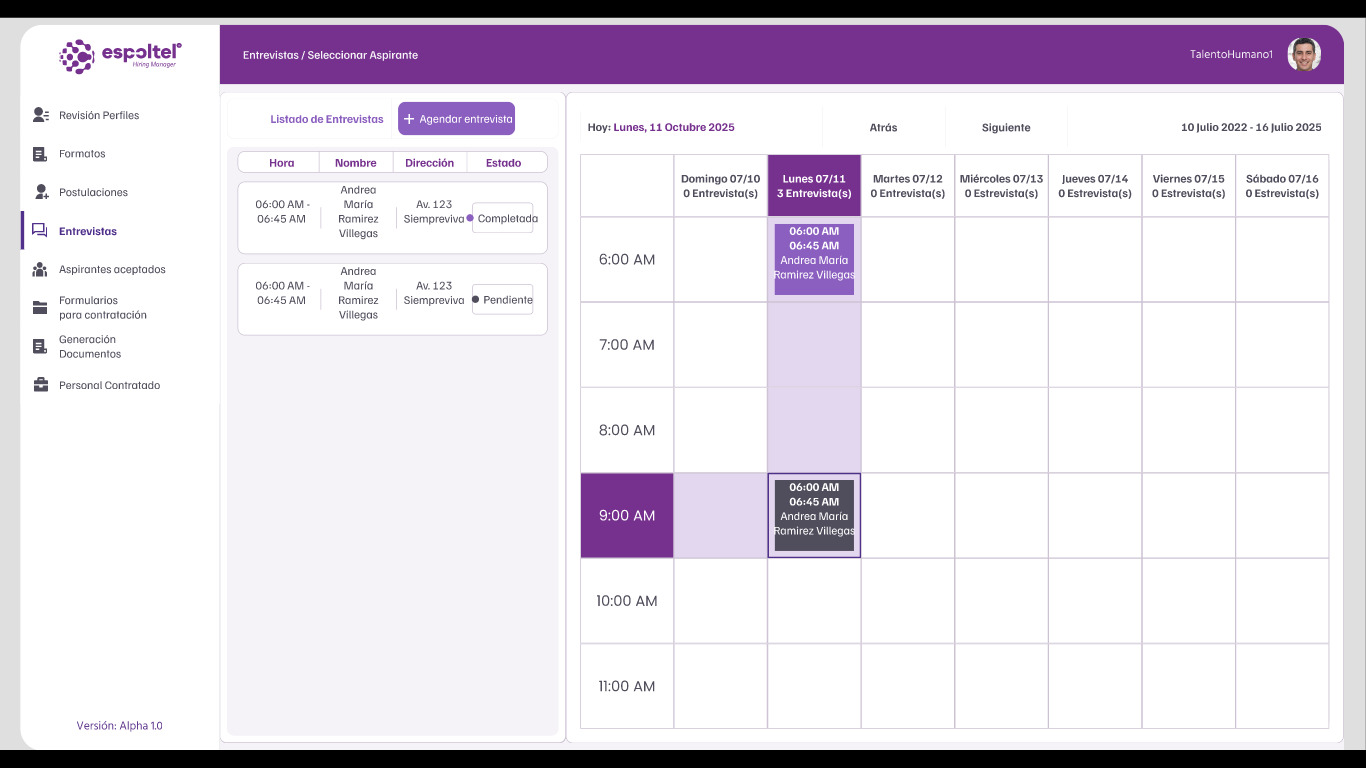
\includegraphics[width=0.8\textwidth]{WebPrototype/wflow-29.jpeg}
	\caption{View of the interviews}
\end{figure}

\begin{figure}[H]
	\centering \small
	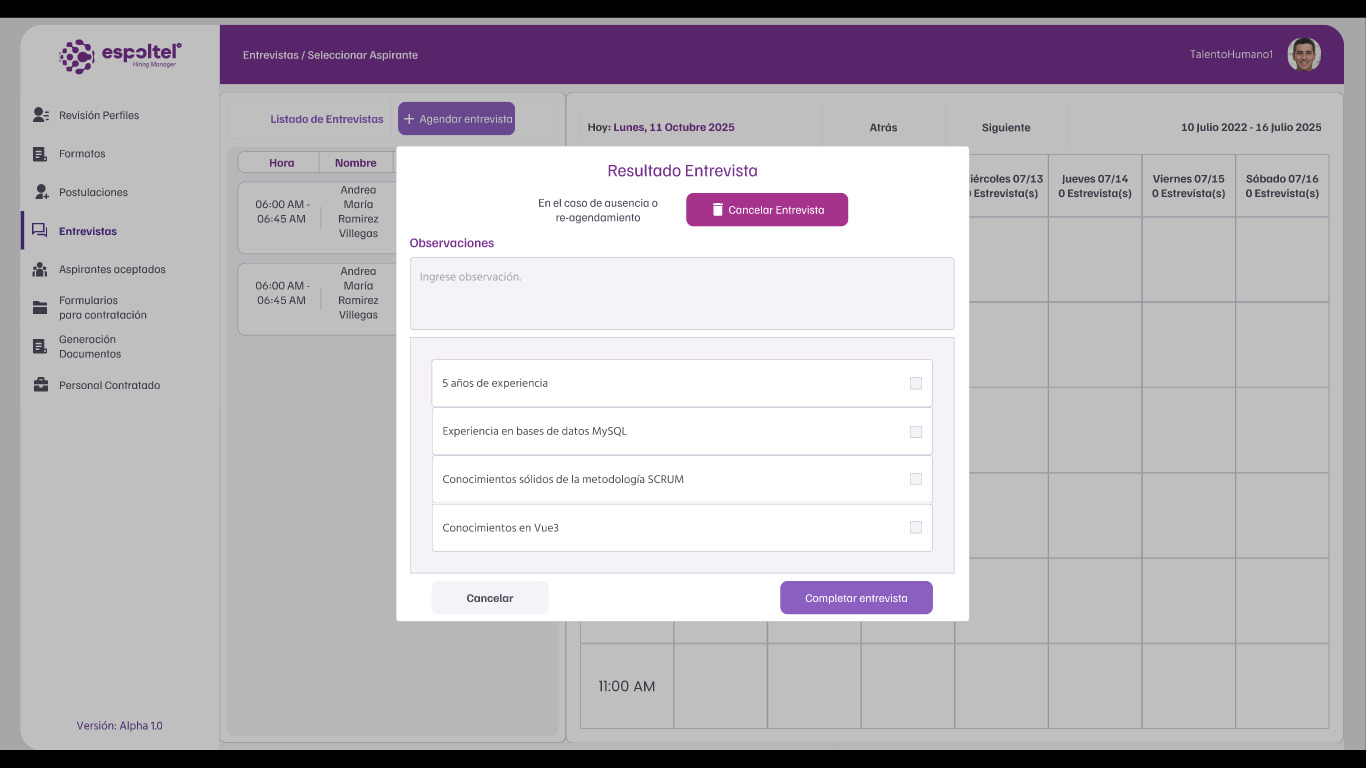
\includegraphics[width=0.8\textwidth]{WebPrototype/wflow-30.jpeg}
	\caption{View of the results of an interview}
\end{figure}

\begin{figure}[H]
	\centering \small
	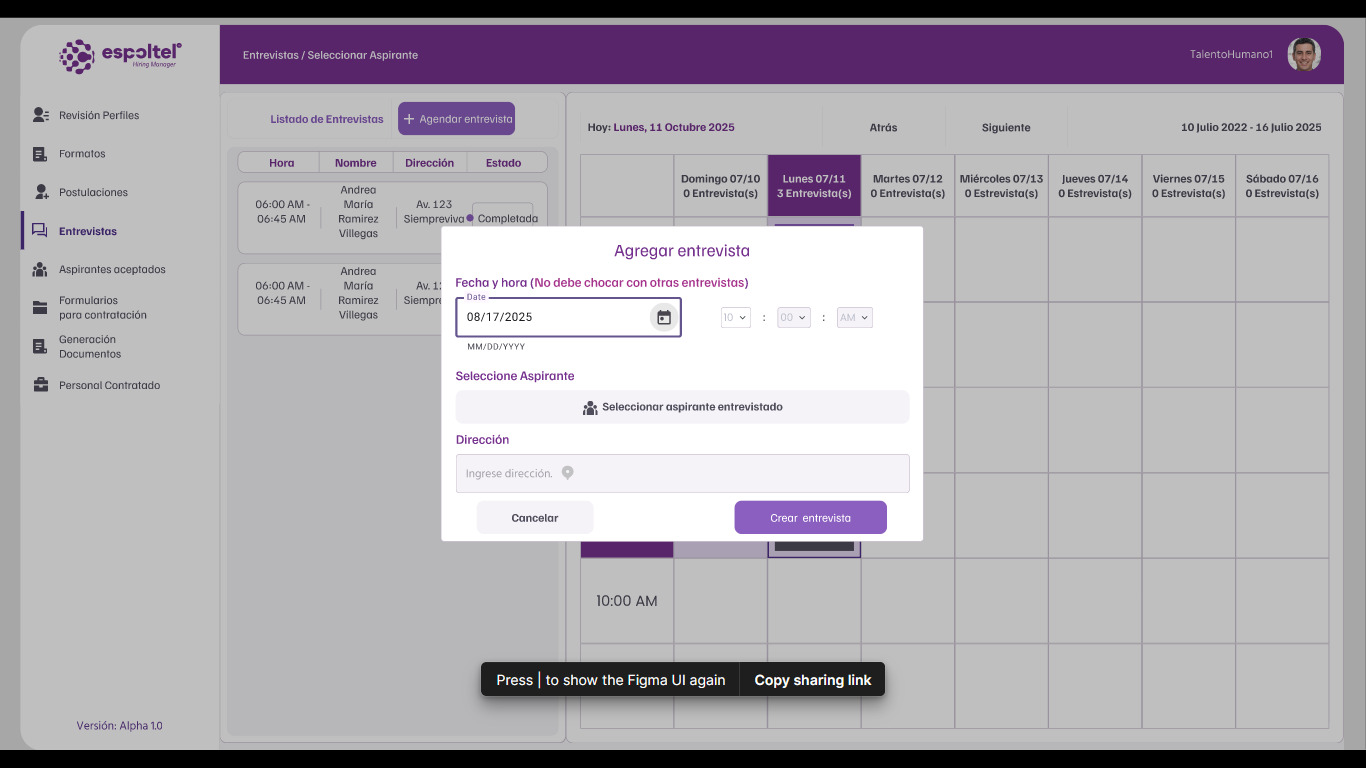
\includegraphics[width=0.8\textwidth]{WebPrototype/wflow-31-2.jpg}
	\caption{View of an interview schedule}
\end{figure}

\begin{figure}[H]
	\centering \small
	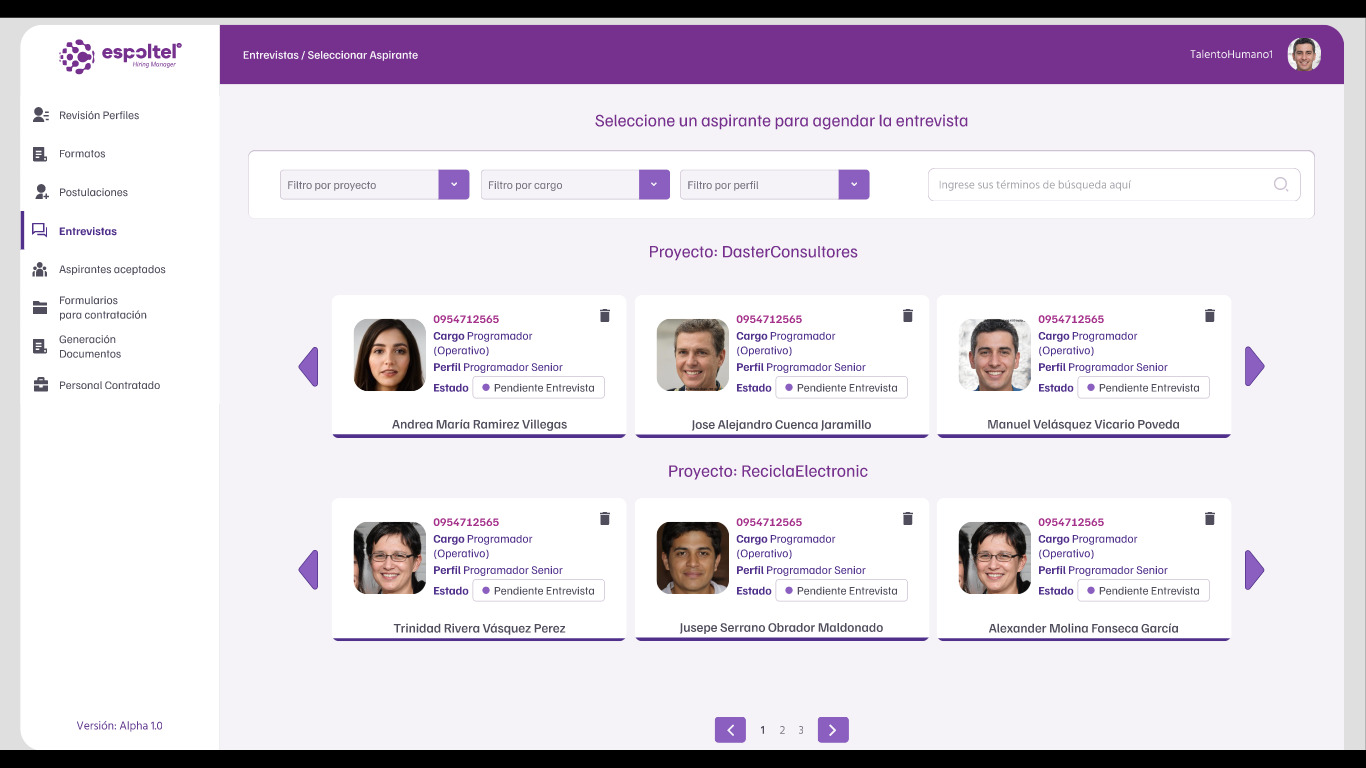
\includegraphics[width=0.8\textwidth]{WebPrototype/wflow-31.jpeg}
	\caption{View of the choice of aspirant to interview}
\end{figure}

\begin{figure}[H]
	\centering \small
	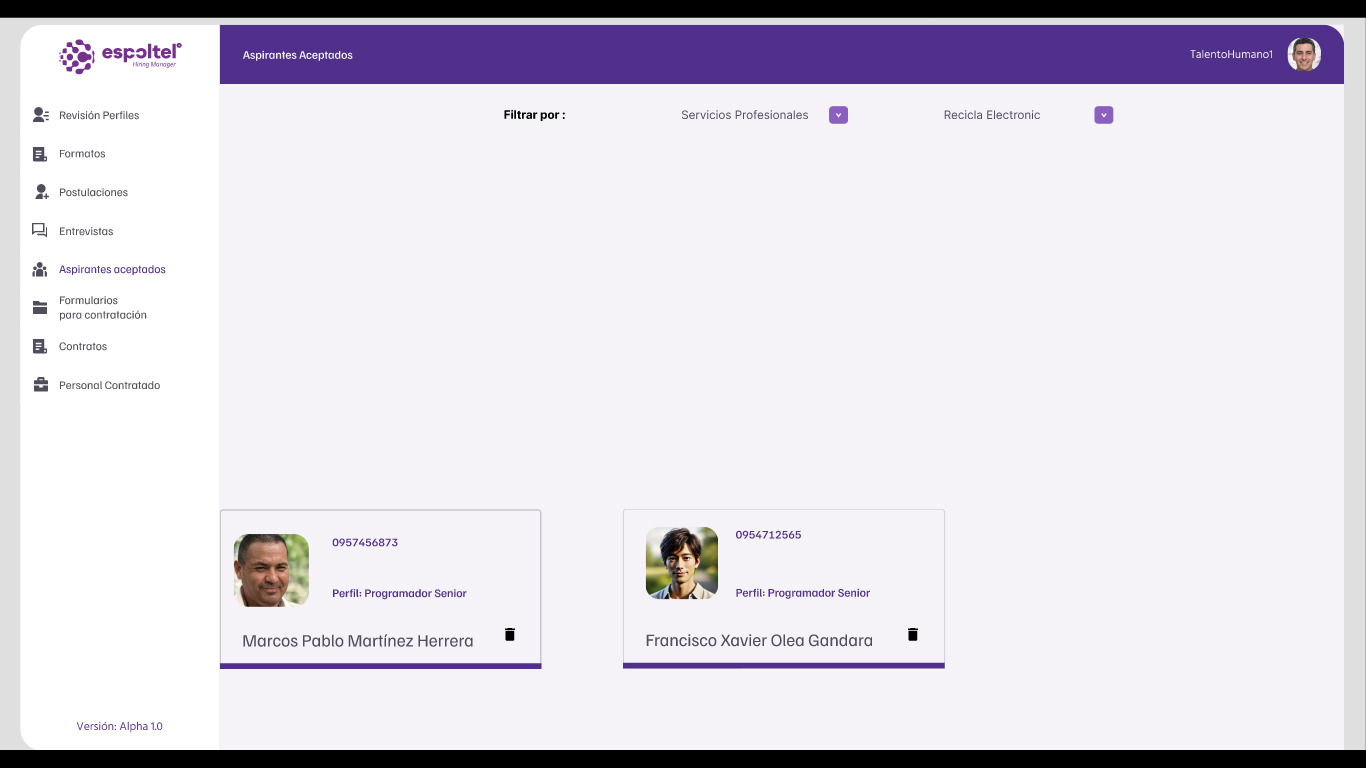
\includegraphics[width=0.8\textwidth]{WebPrototype/wflow-32.jpeg}
	\caption{View of aspirants interviewed}
\end{figure}

\begin{figure}[H]
	\centering \small
	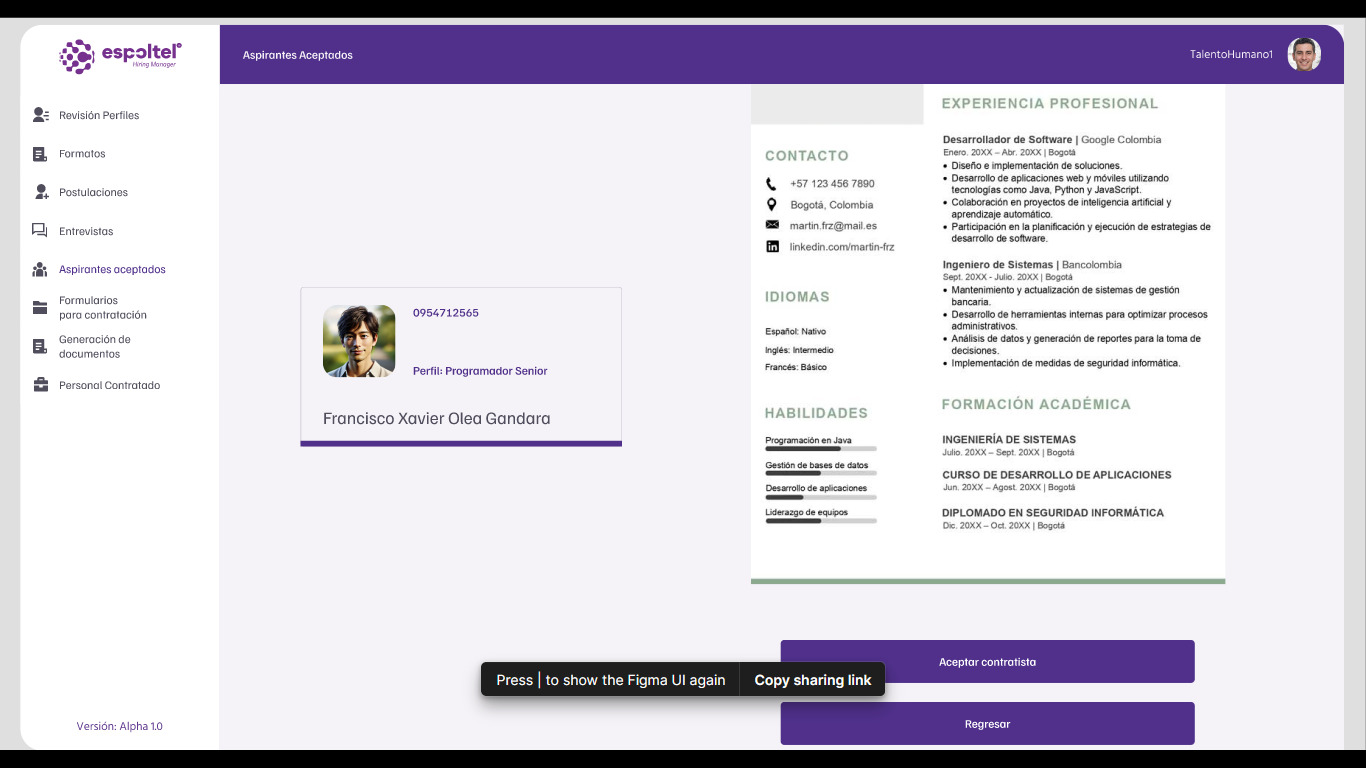
\includegraphics[width=0.8\textwidth]{WebPrototype/wflow-33.jpeg}
	\caption{View of a postulation for acceptance or rejection}
\end{figure}

\begin{figure}[H]
	\centering \small
	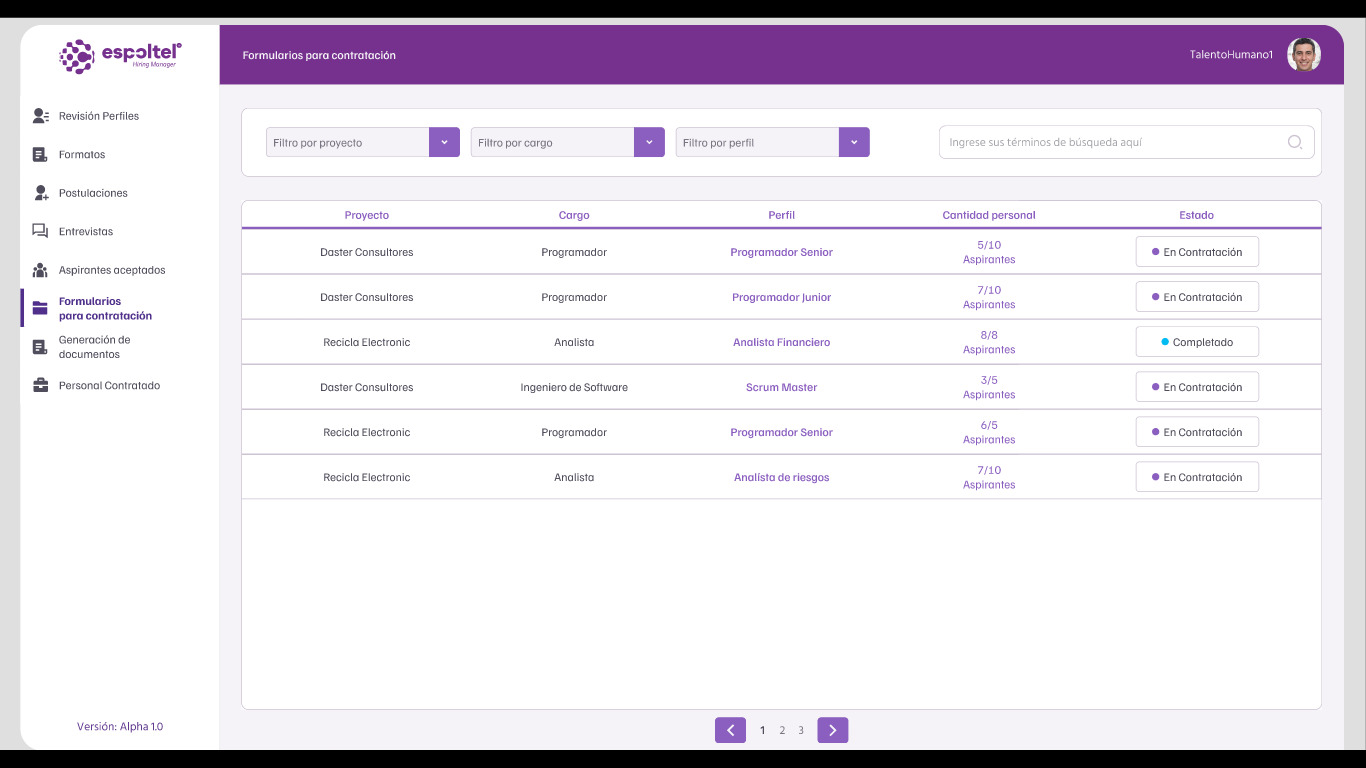
\includegraphics[width=0.8\textwidth]{WebPrototype/wflow-34.jpeg}
	\caption{View of all profiles in hiring}
\end{figure}

\begin{figure}[H]
	\centering \small
	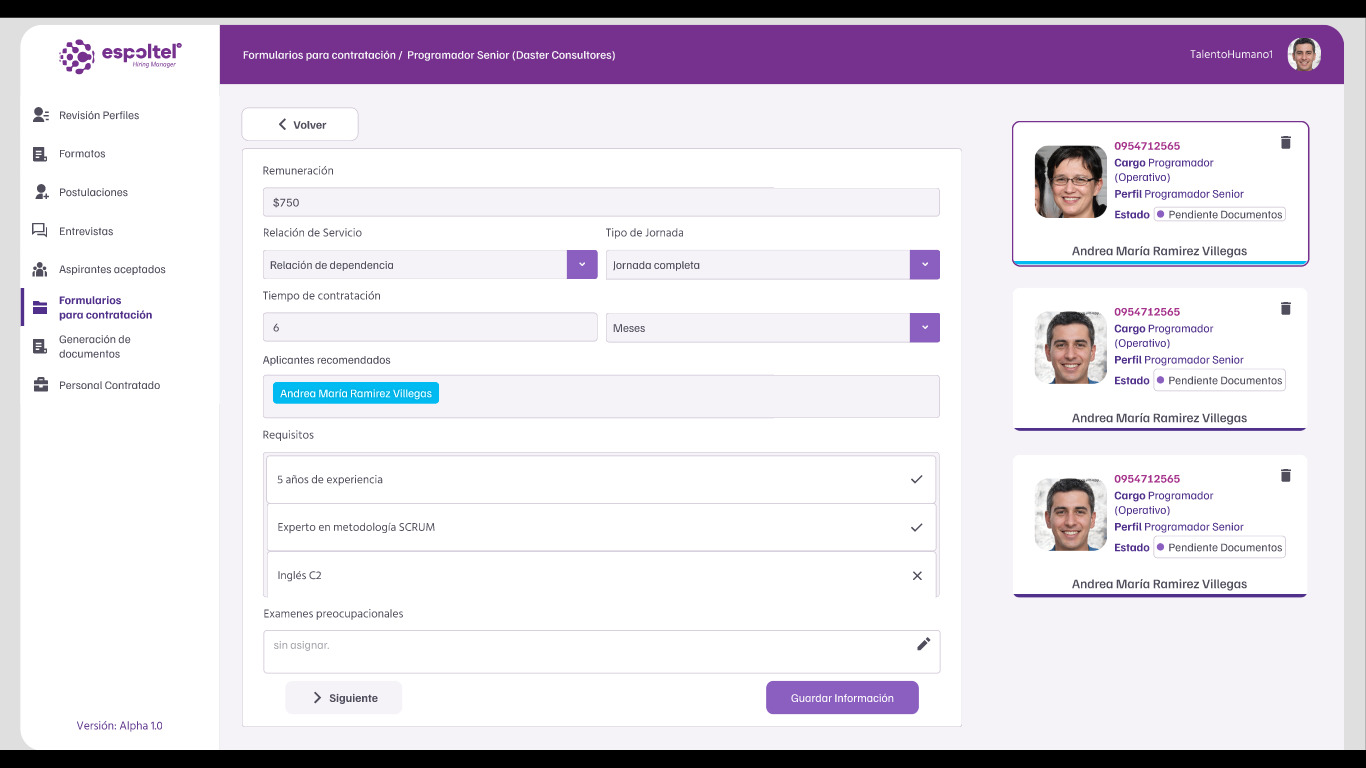
\includegraphics[width=0.8\textwidth]{WebPrototype/wflow-35.jpeg}
	\caption{View of the hiring information of a postulation to a profile to save the information.}
\end{figure}

\begin{figure}[H]
	\centering \small
	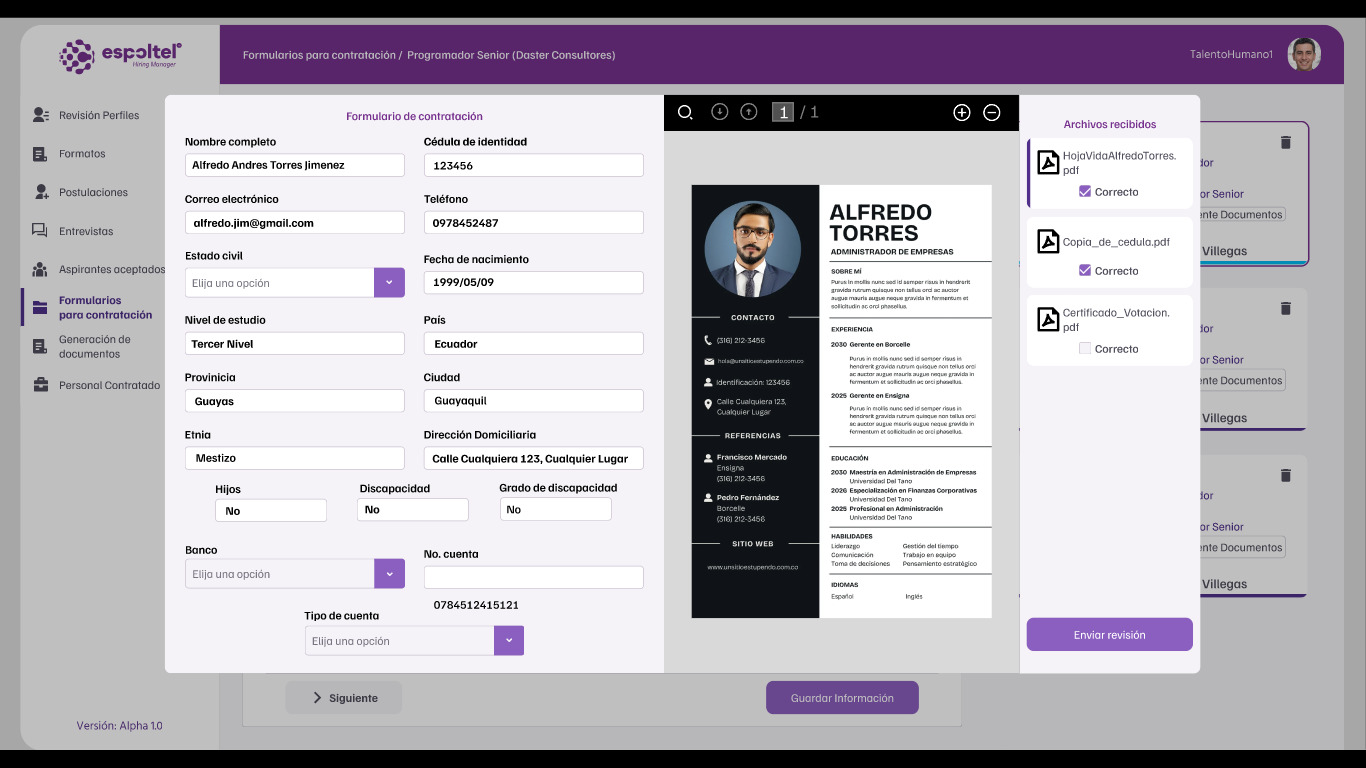
\includegraphics[width=0.8\textwidth]{WebPrototype/wflow-36.jpeg}
	\caption{View of the hiring form received from the aspirant along with his files for hiring.}
\end{figure}

\begin{figure}[H]
	\centering \small
	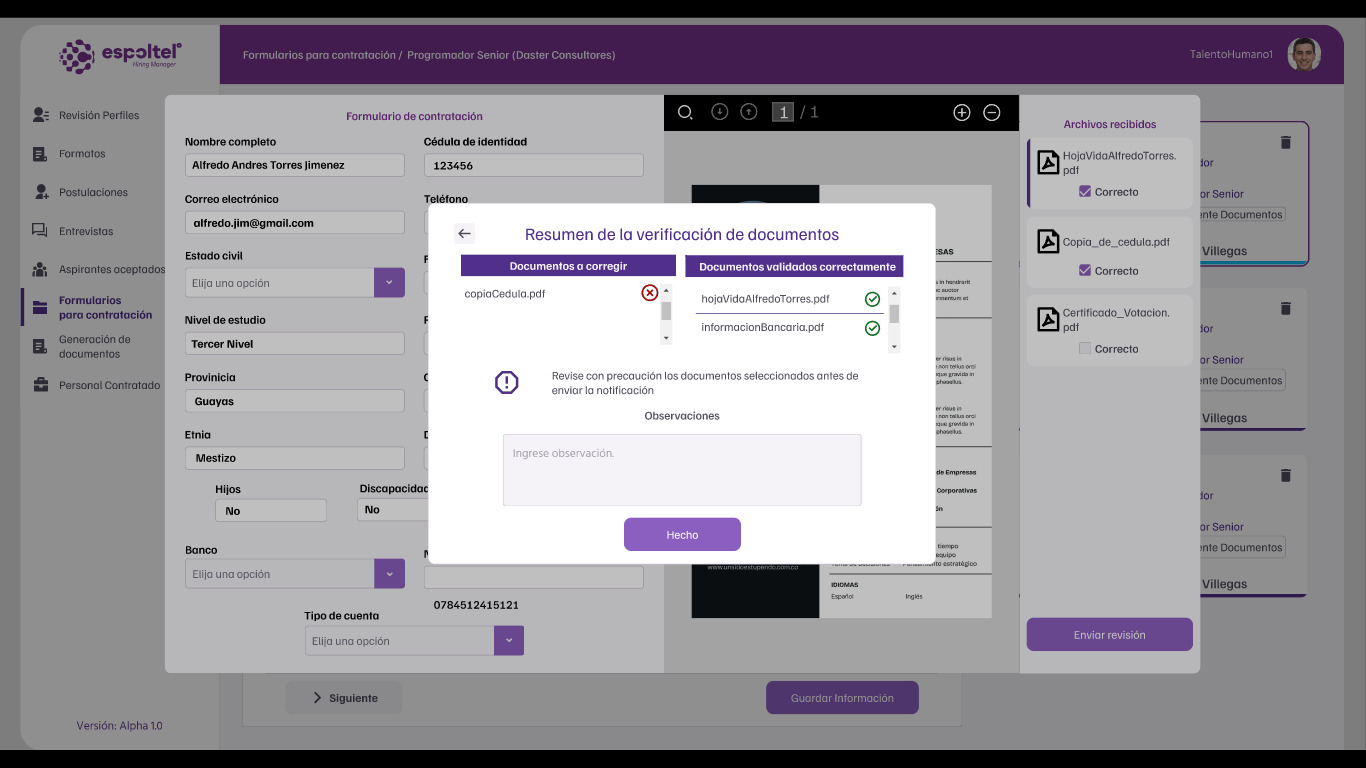
\includegraphics[width=0.8\textwidth]{WebPrototype/wflow-37.jpeg}
	\caption{View of the verification of the contract form}
\end{figure}

\begin{figure}[H]
	\centering \small
	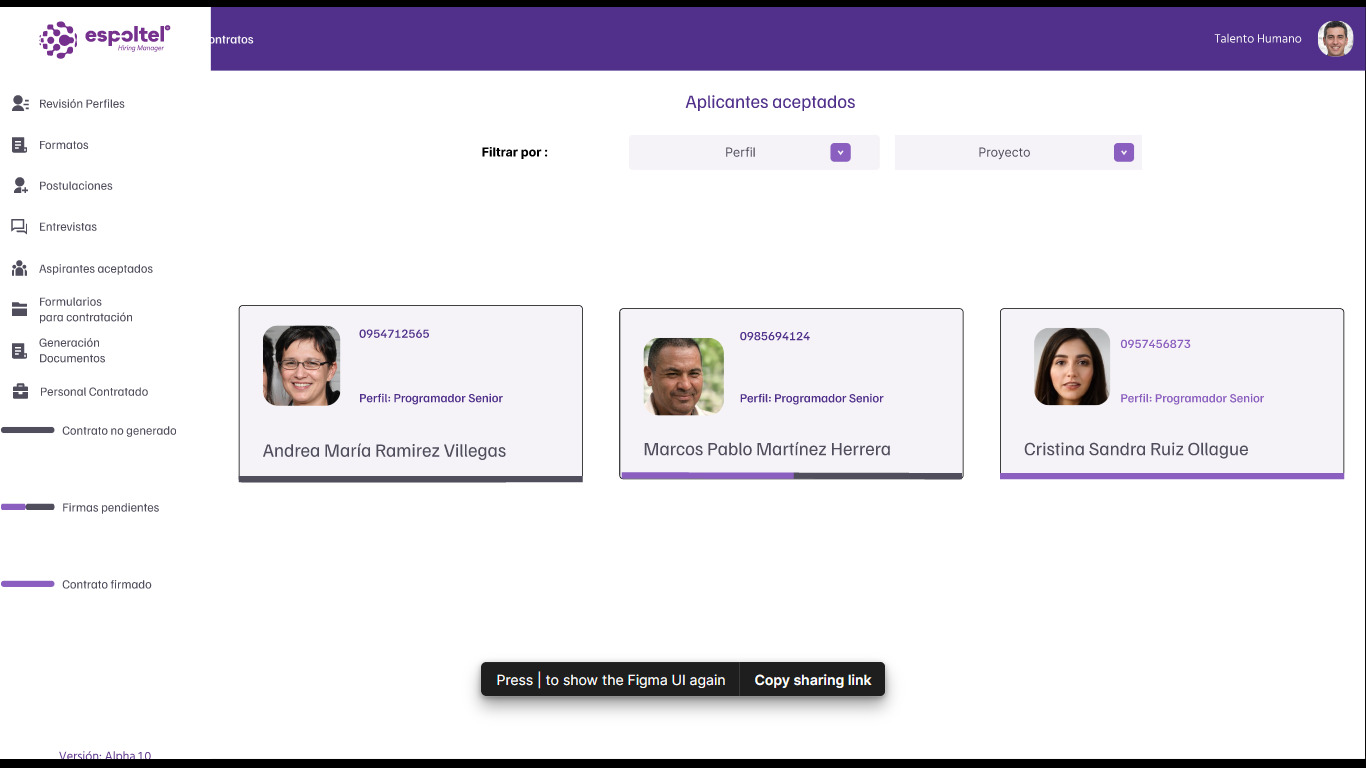
\includegraphics[width=0.8\textwidth]{WebPrototype/wflow-38.jpeg}
	\caption{View of postulations with pending contracts}
\end{figure}

\begin{figure}[H]
	\centering \small
	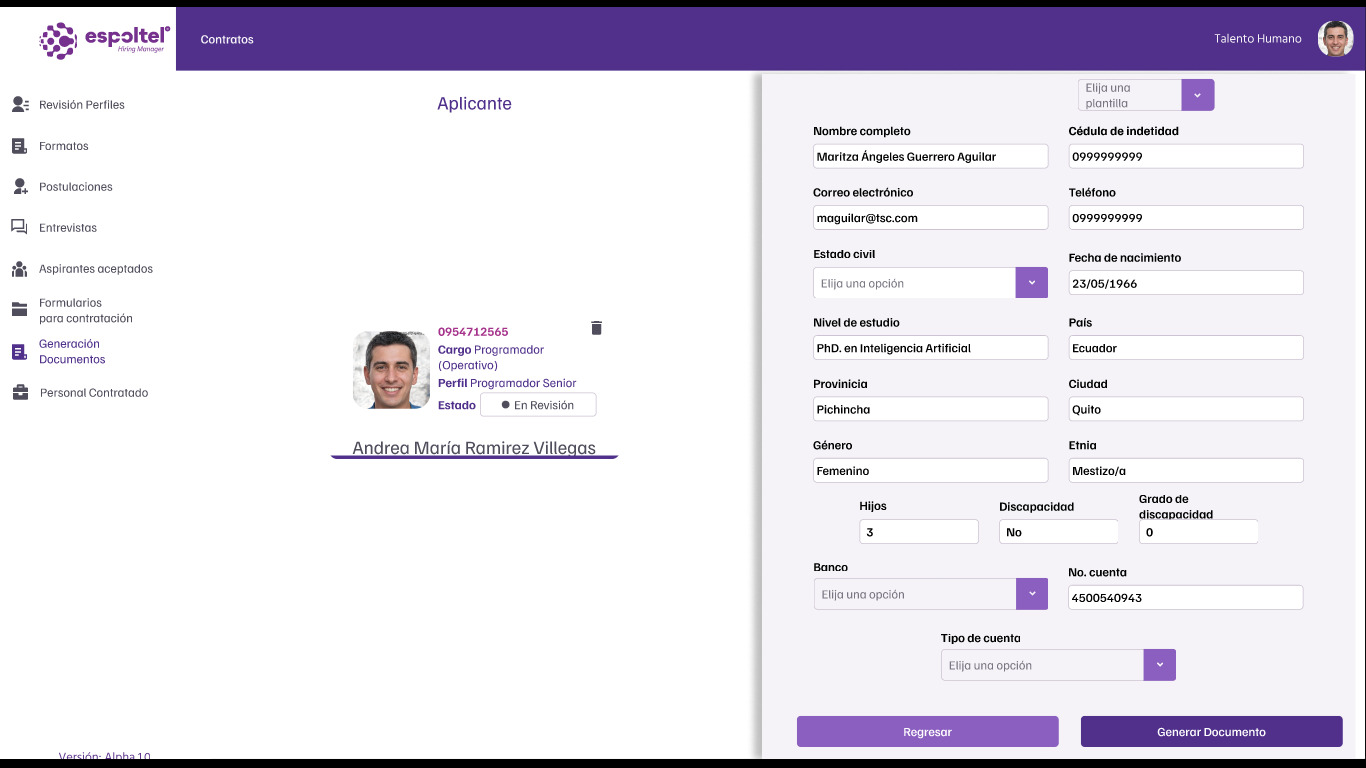
\includegraphics[width=0.8\textwidth]{WebPrototype/wflow-39.jpeg}
	\caption{View of the contract generation of an application}
\end{figure}

\begin{figure}[H]
	\centering \small
	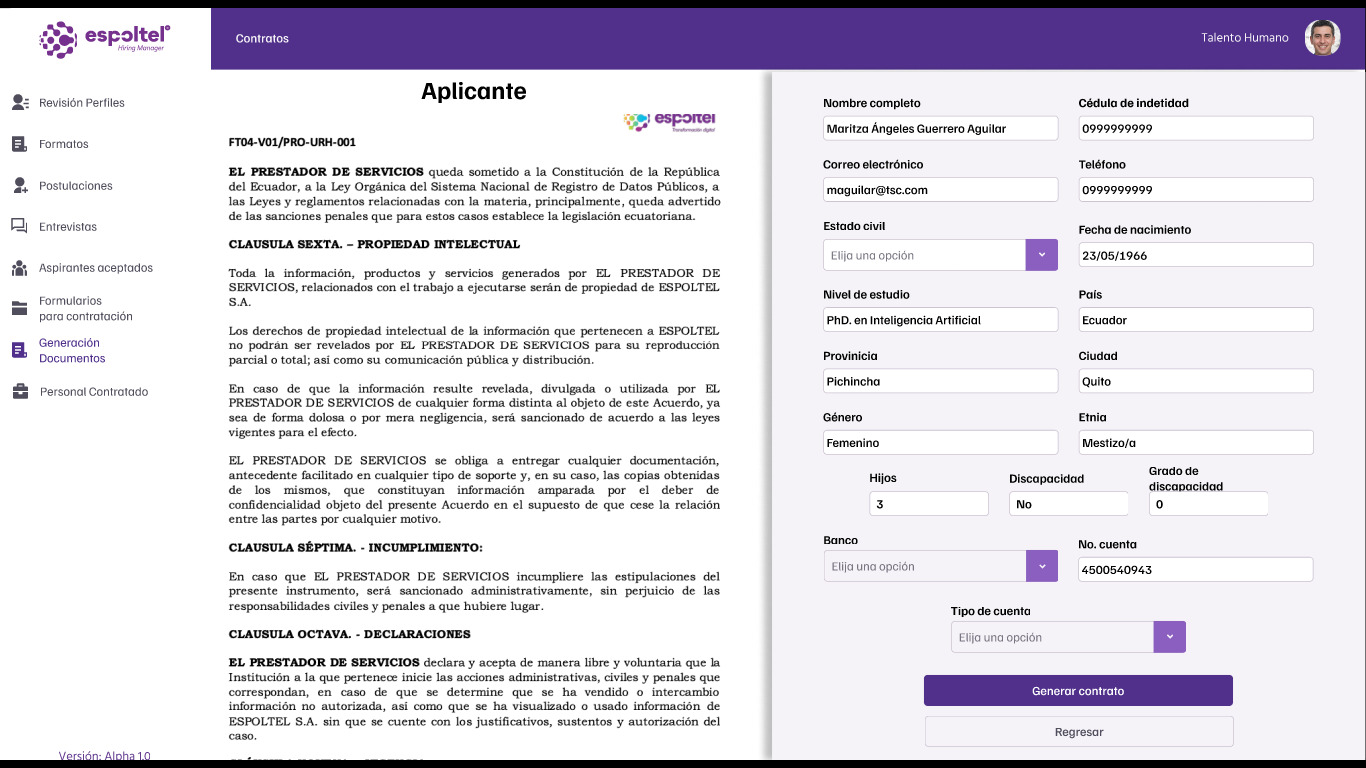
\includegraphics[width=0.8\textwidth]{WebPrototype/wflow-40.jpeg}
	\caption{View of the generated contract to be sent to the aspirant}
\end{figure}

%%
\begin{figure}[H]
	\centering \small
	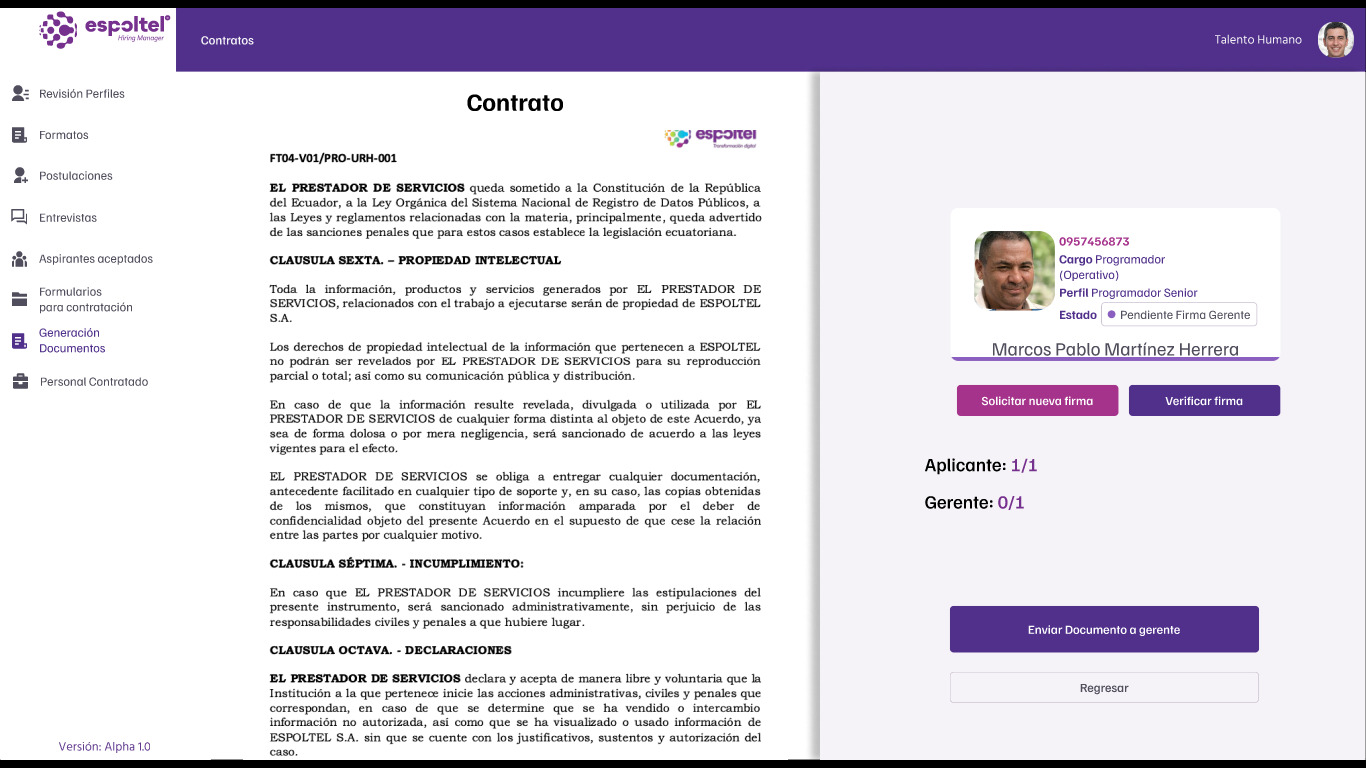
\includegraphics[width=0.8\textwidth]{WebPrototype/wflow-41.jpeg}
	\caption{View of the contract signed by the aspirant ready to validate his signature, and send it to the manager}
\end{figure}

\begin{figure}[H]
	\centering \small
	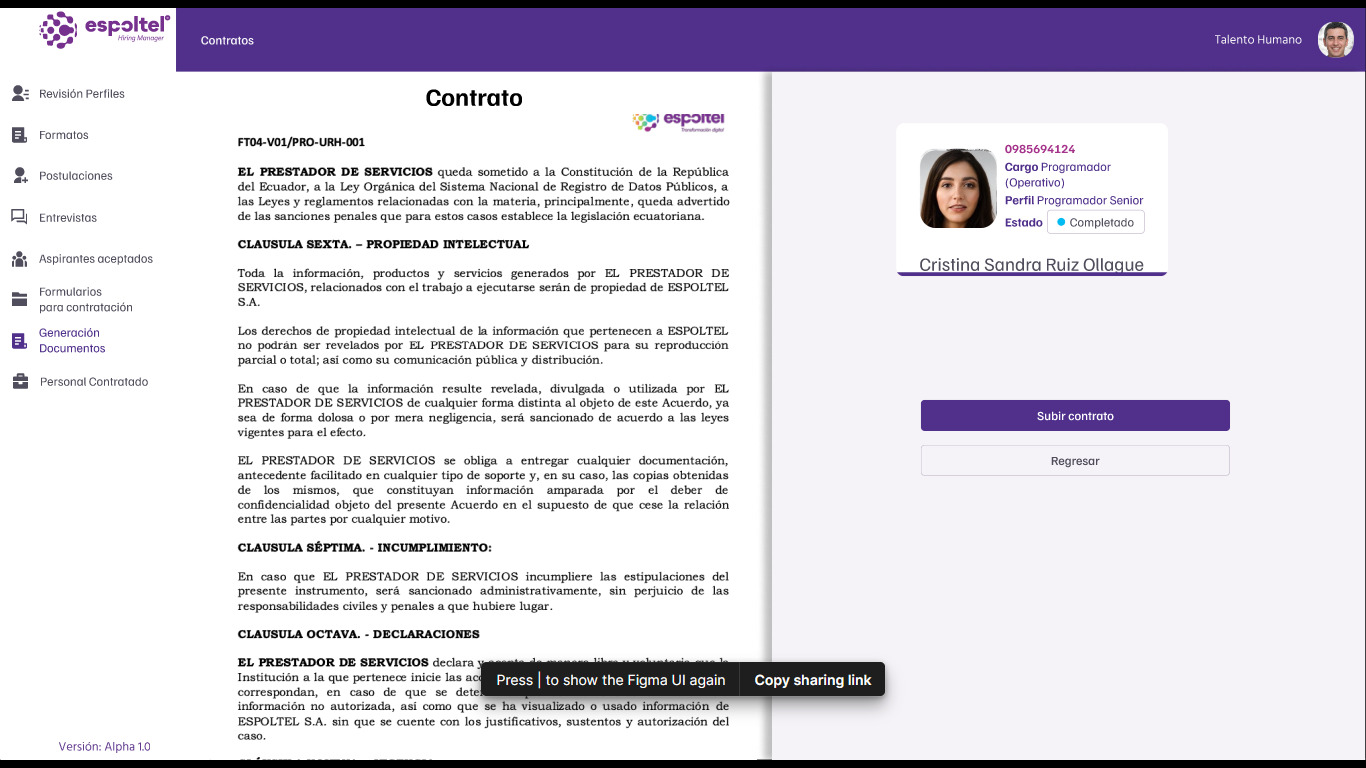
\includegraphics[width=0.8\textwidth]{WebPrototype/wflow-42.jpeg}
	\caption{View of the contract signed by both parties to save it to the system}
\end{figure}

\begin{figure}[H]
	\centering \small
	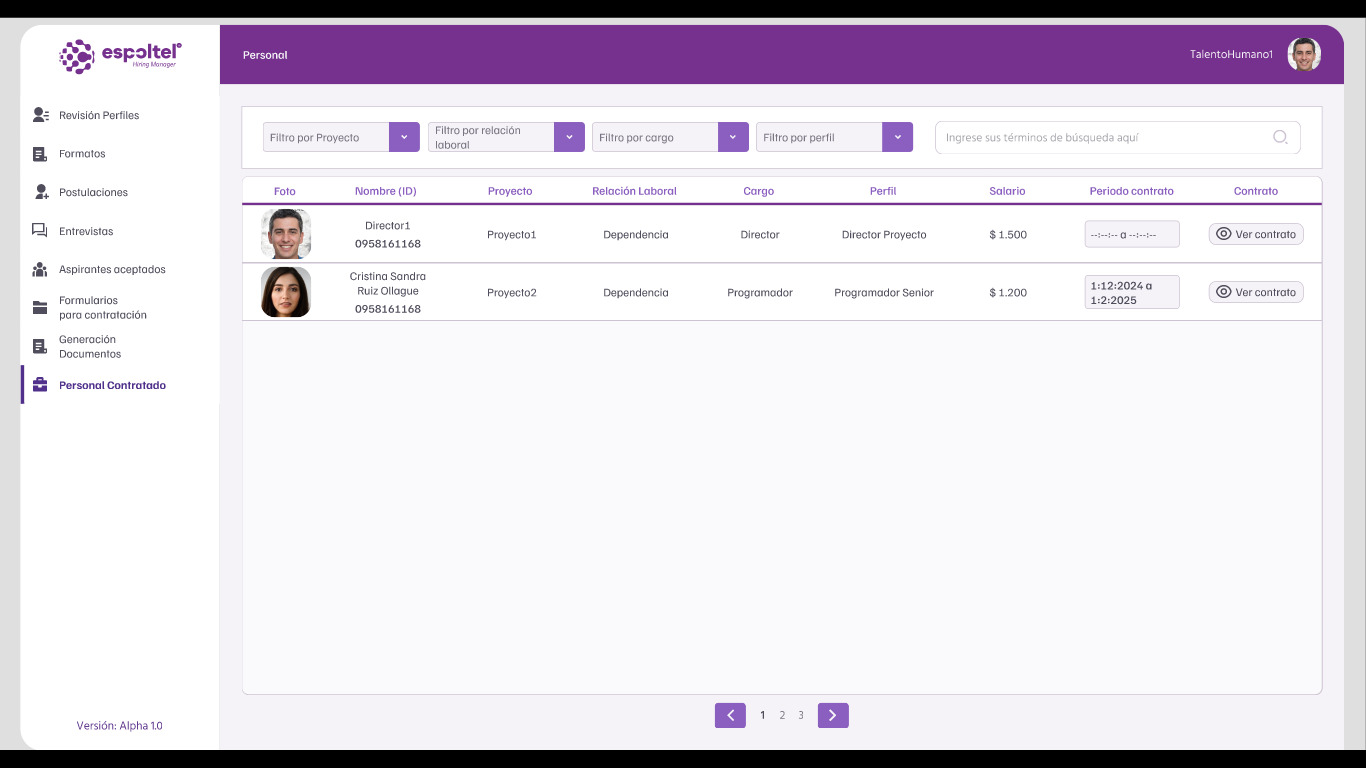
\includegraphics[width=0.8\textwidth]{WebPrototype/wflow-43.jpeg}
	\caption{View of all personnel hired by ESPOLTEL}
\end{figure}

\begin{figure}[H]
	\centering \small
	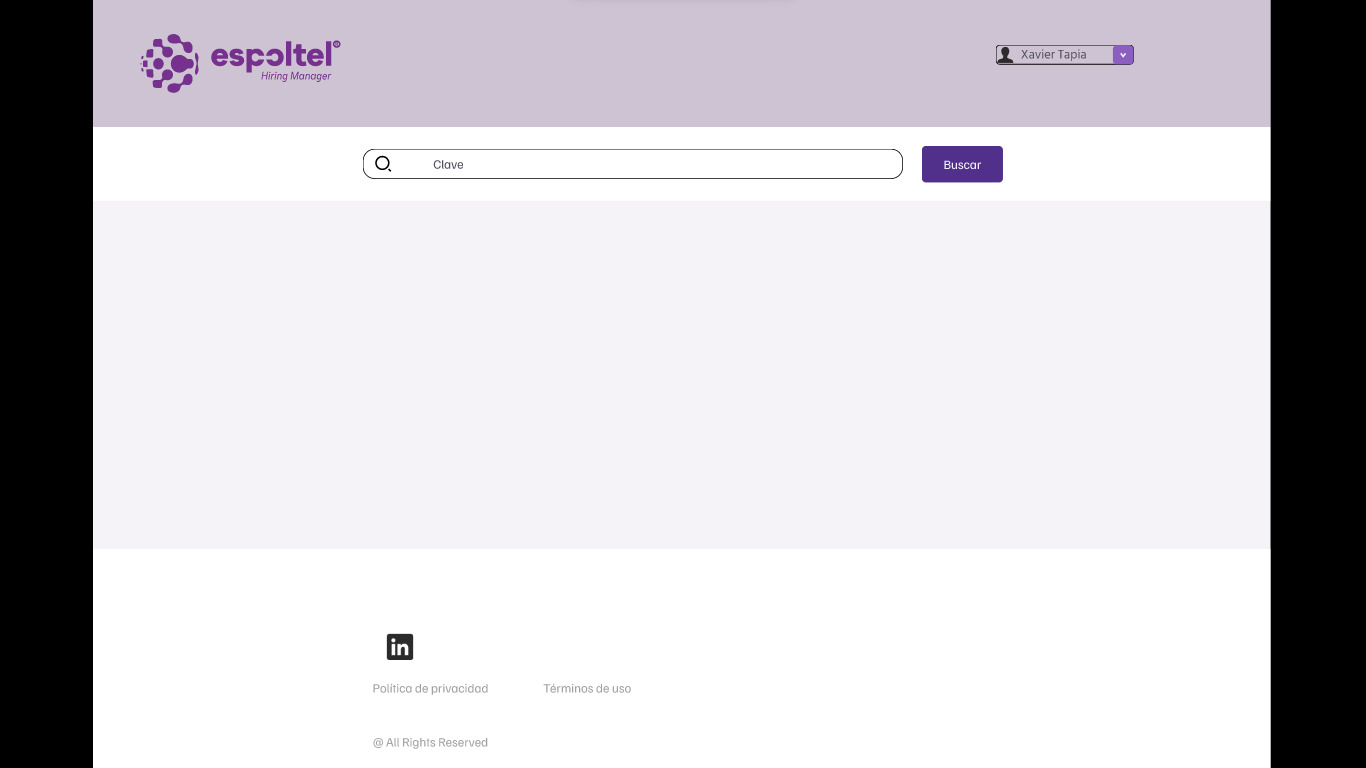
\includegraphics[width=0.8\textwidth]{WebPrototype/wflow-44.jpeg}
	\caption{View of the aspirant's home page}
\end{figure}

\begin{figure}[H]
	\centering \small
	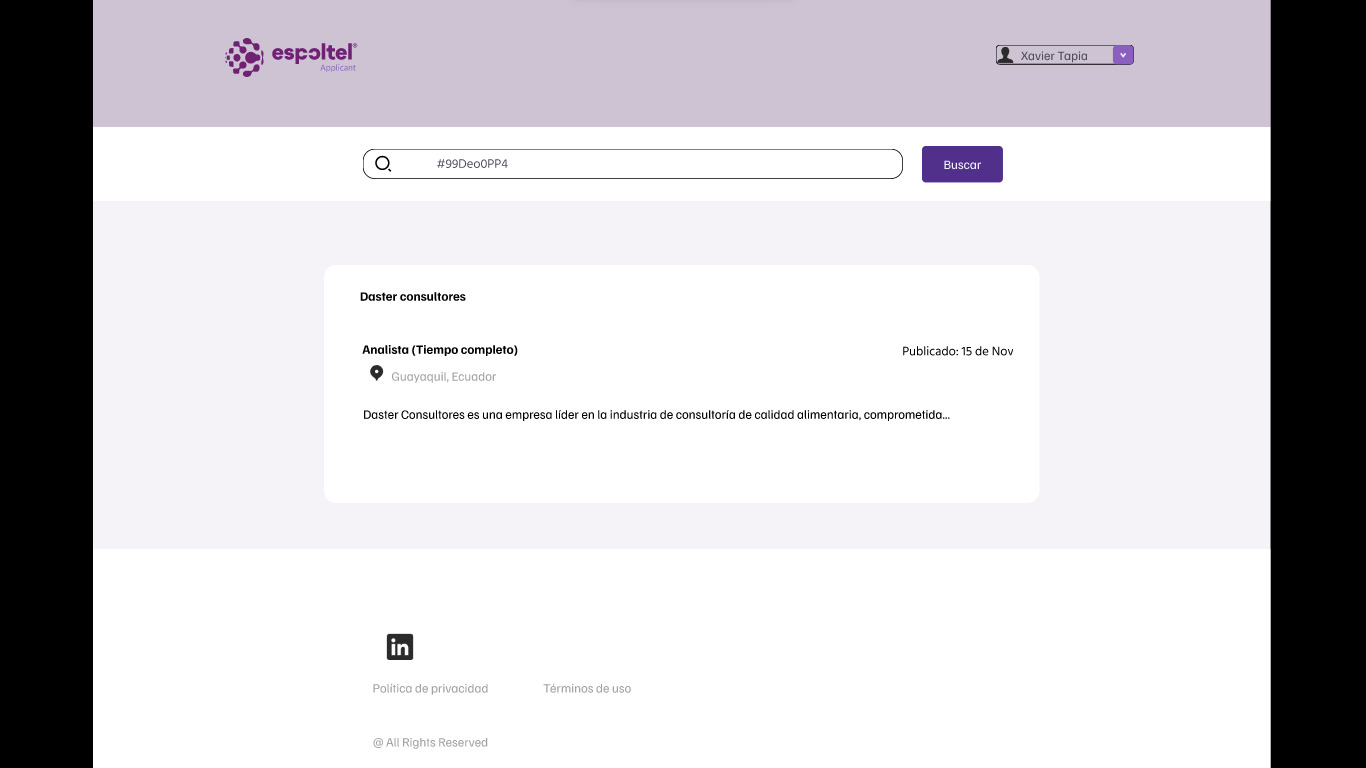
\includegraphics[width=0.8\textwidth]{WebPrototype/wflow-45.jpeg}
	\caption{View of the code entry of a hiring profile}
\end{figure}

\begin{figure}[H]
	\centering \small
	\includegraphics[width=0.8\textwidth]{WebPrototype/wflow-46.jpeg}
	\caption{Detailed view of the position and profile to apply for the position}
\end{figure}

\begin{figure}[H]
	\centering \small
	\includegraphics[width=0.8\textwidth]{WebPrototype/wflow-47.jpeg}
	\caption{View to upload files needed for the initial application, resume and ID, part one}
\end{figure}

\begin{figure}[H]
	\centering \small
	\includegraphics[width=0.8\textwidth]{WebPrototype/wflow-48.jpeg}
	\caption{View to upload files needed for the initial application, resume and ID, part two}
\end{figure}

\begin{figure}[H]
	\centering \small
	\includegraphics[width=0.8\textwidth]{WebPrototype/wflow-49.jpeg}
	\caption{View of postulation confirmation}
\end{figure}

\begin{figure}[H]
	\centering \small
	\includegraphics[width=0.8\textwidth]{WebPrototype/wflow-50.jpeg}
	\caption{View of user information}
\end{figure}

\begin{figure}[H]
	\centering \small
	\includegraphics[width=0.8\textwidth]{WebPrototype/wflow-51.jpeg}
	\caption{View of email and credentials edition}
\end{figure}

\begin{figure}[H]
	\centering \small
	\includegraphics[width=0.8\textwidth]{WebPrototype/wflow-52.jpeg}
	\caption{View of all postulations of an aspirant}
\end{figure}

\begin{figure}[H]
	\centering \small
	\includegraphics[width=0.8\textwidth]{WebPrototype/wflow-53.jpeg}
	\caption{View of aspirant notifications}
\end{figure}

\begin{figure}[H]
	\centering \small
	\includegraphics[width=0.8\textwidth]{WebPrototype/wflow-54.jpeg}
	\caption{View of submitted contract forms}
\end{figure}

\begin{figure}[H]
	\centering \small
	\includegraphics[width=0.8\textwidth]{WebPrototype/wflow-55.jpeg}
	\caption{View of aspirant's contracts}
\end{figure}

\begin{figure}[H]
	\centering \small
	\includegraphics[width=0.8\textwidth]{WebPrototype/wflow-56.jpeg}
	\caption{View of the aspirant's signatory}
\end{figure}


\section{Appendix E: Mobile Application Prototype Screenshots}

%%
\begin{figure}[H]
	\centering \small
	\includegraphics[height=0.5\textwidth]{MobilePrototype/mflow-1.jpeg}
	\caption{View mobile application login page}
\end{figure}

\begin{figure}[H]
	\centering \small
	\includegraphics[height=0.5\textwidth]{MobilePrototype/mflow-2.jpeg}
	\caption{View of the registration inside the mobile application}
\end{figure}

\begin{figure}[H]
	\centering \small
	\includegraphics[height=0.5\textwidth]{MobilePrototype/mflow-3.jpeg}
	\caption{View of the dashboard of the mobile application}
\end{figure}

\begin{figure}[H]
	\centering \small
	\includegraphics[height=0.5\textwidth]{MobilePrototype/mflow-4.jpeg}
	\caption{View of the mobile application sidebar}
\end{figure}

\begin{figure}[H]
	\centering \small
	\includegraphics[height=0.5\textwidth]{MobilePrototype/mflow-5.jpeg}
	\caption{Status view of an postulation}
\end{figure}
%%


\end{document}

